

\documentclass[10pt]{sensys-proc}
\usepackage{graphicx}
\usepackage{balance}
\usepackage{comment}
\newcommand{\redcolor}[1]{\textcolor{red}{#1}}

\newcommand{\figref}[1]{Figure~\ref{#1}}
\newcommand{\secref}[1]{Section~\ref{#1}}
\newcommand{\tabref}[1]{Table~\ref{#1}}
\newcommand{\algoref}[1]{Algorithm~\ref{#1}}
\usepackage{graphicx}
\usepackage{subfig}
\usepackage{blindtext}
\usepackage{array}
\usepackage{caption}
\usepackage{url}
\usepackage{epstopdf}
\usepackage{multirow}
\usepackage{xcolor,colortbl}

\newcommand{\denselistbib}{
  \itemsep -.6pt\topsep-4pt\partopsep-20pt
}

\usepackage{enumitem}

%\setlist{noitemsep,topsep=0pt,parsep=0pt,partopsep=0pt}

\newcommand{\paradigm}{Sense Local-store Upload}
\newcommand{\selstup}{SLsU}

\newcommand{\paradigms}{Sense Local-store Upload~}
\newcommand{\selstups}{SLsU }

\newcommand{\pushline}{\Indp}
\definecolor{Gray}{gray}{0.91}
\newcolumntype{a}{>{\columncolor{Gray}}c}
\newcommand{\superscript}[1]{\ensuremath{^{\textrm{\small{#1}}}}}
\def\sharedaffiliation{\end{tabular}\newline\begin{tabular}{c}}

\def\iiitd{\superscript{\dag}}
\def\ucla{\superscript{\S}}
\setlength{\belowcaptionskip}{-10pt}

\setlength{\parskip}{0pt}
%\setlength{\parsep}{0pt}
%\setlength{\headsep}{0pt}
%\setlength{\topskip}{0pt}
%\setlength{\topmargin}{0pt}
%\setlength{\topsep}{0pt}
%\setlength{\partopsep}{0pt}
%\linespread{0.5}



\numberofauthors{1}

\author{
\alignauthor 
	Nipun Batra\iiitd, 
	Manoj Gulati\iiitd, 
	Amarjeet Singh\iiitd, 
	Mani B. Srivastava\ucla
%\alignauthor Pandarasamy Arjunan\\
\sharedaffiliation
  \begin{tabular}{ccc}
    \affaddr{{\iiitd}Indraprastha Institute of Information Technology{\ }} & & \affaddr{{\ucla}University of California{\ }} \\
    \affaddr{Delhi, India}                  & & \affaddr{Los Angeles, United States} \\
\email{\{nipunb,manojg,amarjeet\}@iiitd.ac.in} & & mbs@ucla.edu
  \end{tabular}
}
\vspace{-3mm}
\title{It's Different: Insights into home energy consumption in India\vspace{-3mm}}
\crdata{978-1-4503-1169-4}
\conferenceinfo{Buildsys'13,} {November 11--15, 2013, Rome, Italy.}
\CopyrightYear{2013}

\begin{document}


\maketitle


\begin{abstract}
\looseness -1 Residential buildings contribute significantly to the overall energy usage across the world. Real deployments, and collected data thereof, play a critical role in providing insights into home energy consumption and occupant behavior. %, thus paving the way for building systems that can reduce energy consumption. 
Existing datasets from real residential deployments are all from the developed countries. Developing countries, such as India, present unique opportunities to evaluate the scalability of existing research in diverse settings. Building upon more than a year of experience in sensor network deployments, we undertake an extensive deployment in a home in Delhi, measuring electrical, water and ambient parameters. Our ongoing deployment was started on $25^{th}$ May 2013. Since then, 33 sensors have been collecting a total of approx. 400 MB of data daily, across the aforementioned modalities.  We discuss the architectural implications on the deployment systems that can be used for monitoring and control in the context of developing countries. Addressing the unreliability of electrical grid and internet in such settings, we present \emph{\paradigms} architecture for robust data collection.
% suited to the context of deployments in developing countries.
While providing several unique aspects, our deployment further validates the common considerations from similar residential deployments, discussed previously in the literature. %We discuss architectural implications towards development of building monitoring and control systems, that can scale across diverse deployment settings. %, prevailing in both developed and the developing countries.
\end{abstract}

% A category with the (minimum) three required fields
\category{H.4}{Information Systems Applications}{Miscellaneous}
%A category including the fourth, optional field follows...
\category{D.2.8}{Software Engineering}{Metrics}[complexity measures, performance measures]

\terms{Design, Experimentation}

\keywords{Deployment, Buildings, Smart Homes, Sensor Networks}

\vspace{-1mm}
\section{Introduction}
\label{sec:intro}
\looseness -1 Buildings account for more than 30\% of overall energy consumption globally. %The contribution of buildings to overall energy usage for different countries is as follows- Australia: 20\%, China: 34\%, India: 47\%, Japan: 33\% and USA: 29\%. 
Of this energy consumption, a large proportion (e.g. 93\% in India) is contributed by residential buildings~\cite{evans09india}. %contribute significantly to overall building energy usage (China: 90\%, India: 93\%, Australia: 67\%)~\cite{evans09aus,evans09us,evans09japan,evans09india,evans09china}.
Information Technology (IT) such as cyber-physical systems, wireless sensor networks, embedded control, computational modeling, machine learning, and simulation tools can play a key role in reducing the net energy resources consumed in a building while maintaining the productivity of its occupants. These IT methods include guiding the occupants towards resource conserving behaviors, alerting for timely repair of energy-wasting degradations in building facilities, intelligent control of the building systems, and opportunistically harvesting energy from the environment.
 
\looseness -1 Of particular importance are the systemic building deployments that can provide detailed insights about occupant behavior (specifically, Activities of Daily Living (ADLs)) and energy consumption. These deployments also provide data sets that can be leveraged for developing and testing suitable control strategies. These control strategies are otherwise complex to undertake in a real occupied building. In the recent past, several datasets, such as REDD~\cite{redd}, BLUED~\cite{blued_cmu}, Smart*~\cite{smart}, monitoring household electricity and ambient parameters, have been released publicly. Several building monitoring and control research has since used these datasets to prove the validity of their work for real life settings~\cite{parson2012_aaai,smartcap}.  

\looseness -1 However, all of the previous deployments have been done in the context of developed countries. Developing countries, such as India, have higher electricity deficit, are adding new building space at a higher rate and constitute different infrastructure and energy consumption patterns. A deeper understanding of these different settings in developing countries can help in the development of systems that can scale across diverse settings in a robust manner. %, it is equally important to understand building energy consumption in developing countries such as India, where there is electricity deficit and new buildings are being constructed at a rapid rate, adding to electricity demand. The peak demand deficit in India was reported to be 10.3\% in the year 2010-2011~\cite{india_energy_book}. Also, 19 million square meters of residential building space was added in 2004-2005~\cite{evans09india}.
We have been involved in sensor network deployments in the Indian context for more than a year~\cite{batra}, whereby, we have instrumented 25 homes with smart meters, a smart campus with sensors for ambient monitoring in a research wing and 52 smart meters in the institute dorms. In this paper, we discuss an extensive ongoing deployment in a home in Delhi, India, started on $25^{th}$ May 2013. Monitored parameters include electricity and water consumption at the meter level, plug level load monitoring for major appliances, and ambient parameters across every room. We used 33 sensors across the 3 storey home to measure the parameters mentioned above, collecting approx. 400 MB data everyday.%, among others. 

\looseness -1 To the best of our knowledge, this is the first such extensive deployment outside any developed country. We discuss, in detail, the unique aspects of our deployment that are also characteristic of buildings in the developing countries. Correspondingly, we provide insights into these aspects, of building systems, critical for robust data collection and control. We further discuss aspects of our deployment that were similar to those highlighted in the previous work on residential deployments. Our deployment was maintained as an open source project, clearly illustrating the issues faced and how these were addressed. Unlike many of the past deployments, detailed metadata logs, such as appliance make and mode of operation, are also provided. We believe that the unique aspects of the building energy infrastructure, as discussed in this work, will enrich the existing research in building energy domain, which has only leveraged deployments and data collection in the context of developed countries until now. %, for wider applicability across different contexts. 
%\redcolor{I think we should explicitly enumerate our main contributions}

\vspace{-1mm}
\section{Related Work}
\looseness -1 Building deployments have been studied in the past with the goal of improving the building energy efficiency. Office and campus deployments presented in the previous work \cite{yuvraj_ipsn,batra} have shown the scope for significantly reducing HVAC and plug load energy consumption in respective settings. Several other deployments target residential sensing for modeling and inference, specifically pertaining to Non Intrusive Load Monitoring (NILM). Kolter et al.~\cite{redd} performed deployments across 6 homes in Boston (US) in 2011, with collected data spanning up to 19 days in some homes. They monitored household electricity at the meter, circuit and appliance level using Commercial Off-The-Shelf (COTS) devices. Their dataset (REDD) has been frequently used to validate NILM research and to date has been cited 57 times, clearly suggesting the impact of such deployments. Anderson et al.~\cite{blued_cmu} performed a week long residential deployment, specifically focusing on collecting fully labeled high frequency electrical data and released BLUED dataset. Our data, in comparison, is for a much longer duration (spanning 73 days at the time of writing), uses a mix of COTS and customized hardware (due to non-availability of COTS, for everything we wanted to monitor, in the Indian context), and provides a unique combination of electricity, water consumption and ambient parameters.

\looseness -1 Barker et al.~\cite{smart} performed deployments across three homes and have collected information across varying modalities including, but limited to, electricity consumption, occupancy, weather and renewable electricity generation. They illustrated the wide applicability of the data from their residential deployment, including peak demand flattening~\cite{smartcap} and cost optimization using variable electricity pricing~\cite{smartcharge}. They further highlighted the value of additional information obtained by correlating across multiple sensing modalities. Motivated by this work, we decided to monitor the ambient parameters, in addition to monitoring electrical and water consumption at different granularity. %Our deployment further provides insights into unique aspects of building energy consumption in the Indian context.

\looseness -1 Hnat et al.~\cite{hitchhiker_residential} provide a detailed guide into residential deployments and provided lessons learned from residential deployments across multiple homes for several years. They proposed various applications of such detailed sensing including identifying ADLs. While providing unique aspects of our deployment, we further establish the commonalities in our deployment with the learning discussed in their work. %Previous residential deployments have also led to smarter appliances such as smart thermostat~\cite{smart_thermostat}, which builds probabilistic models on data collected from door and motion sensors, to build an electricity efficient thermostat.
To the best of our knowledge, all the deployments discussed previously in the literature pertain to the developed countries. While residential deployments anywhere across the world are challenging, our deployments highlight some unique challenges specific to the developing countries. Some of these challenges in our setting include, but are not limited to, unreliable grid, unreliable internet and difficulty in procuring quality COTS.

\vspace{-1mm}
\section{Deployment Overview}
%Over the past year, we have performed extensive sensor deployment for ambient monitoring in research environment and smart meters across more than 25 homes in India. 
Our deployment constitutes 33 sensors measuring electricity, water and ambient parameters at different granularity, in a home in Delhi, India during May-August 2013. Primary objective for this deployment was to bring forth the differences in the Indian context, as compared to the context of developed countries along the dimensions of - 1. The ecosystem of available sensing options that restrict the possible deployments; 2. Energy and water consumption patterns; and 3. Grid and network reliability. \figref{fig:overall} shows the deployment of these sensors in a 3 storey home, together with the required computing and communication infrastructure. %5 single board computers and 3 routers for computing and communication. We now provide detailed description for our deployment.

\begin{figure} 
	\vspace{-4mm}    
    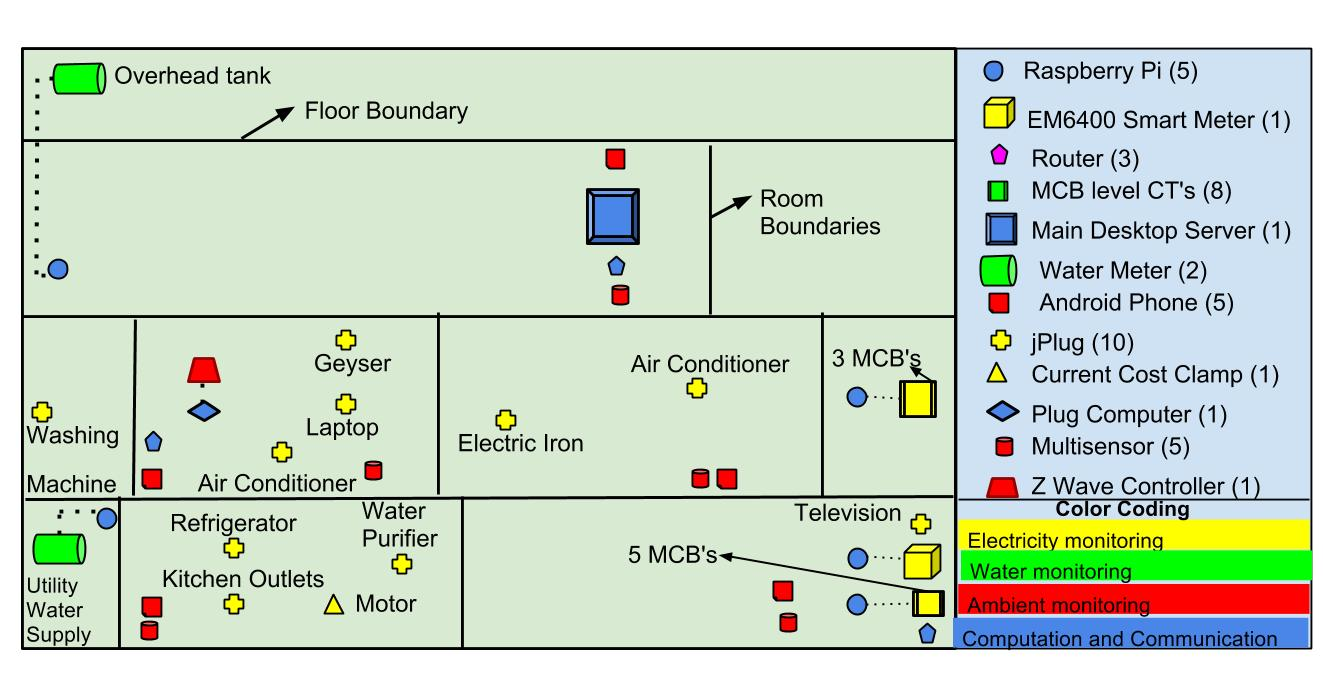
\includegraphics[scale=0.19]{./figures/overall_deployment.jpg}
    \vspace{-10mm}    
    \caption{Schematic showing overall home deployment} 
    \vspace{-2mm}  
    \label{fig:overall}
\end{figure}

\subsection{Sensing Infrastructure}
\label{sec:sensing}
For sensing, we took a ``leave no stone unturned'' approach, where  we chose to monitor as many physical (ambient conditions, electricity usage and water usage) and non-physical (such as network strength and network connectivity) parameters as possible. We took care to deploy these sensors in a way that residents can continue their daily routines without added inconvenience. Constrained by the limited options available in the Indian context, our sensors constitute COTS (procured from both within and outside India) and custom built hardware. %Detailed description of the sensors used for monitoring various parameters are explained next.

\noindent\textbf{Electricity monitoring:} %A typical home electricity setup involves a meter which is installed by utility companies and measures overall electricity usage. Further electric cabling is divided into various Miniature Circuit Breakers (MCB's) which control separate circuits. Typical installations involve putting a separate MCB for each heavy load (such as air conditioners) and clubbing various lights, fans and other smaller loads into separate MCB's. Further each individual appliance is controlled via a switch. There are two types of appliances- i) plug loads like refrigerator and electric iron, which need to be physically ``plugged" into the sockets; ii) loads like lights and fans, which do not need to be ``plugged" in by the user and can directly be switched on or off. We highlight the above described home electricity distribution in \figref{fig:electricity_distribution}. 
Motivated by prior electricity consumption deployments, we also chose to monitor electricity consumption across different granularity - electricity meter monitoring the consumption at the home aggregate level, current transformers (CTs) monitoring current for Miniature Circuit Breakers (MCBs) (each connected to a combination of appliances) and plug level monitors for monitoring plug load based appliances (see \figref{fig:electricity_distribution} for illustration). 
\begin{figure*}[t!] 
    \vspace{-10.5mm}
    \subfloat[\scriptsize EM6400 Smart Meter]{
    \label{fig:em6400}
    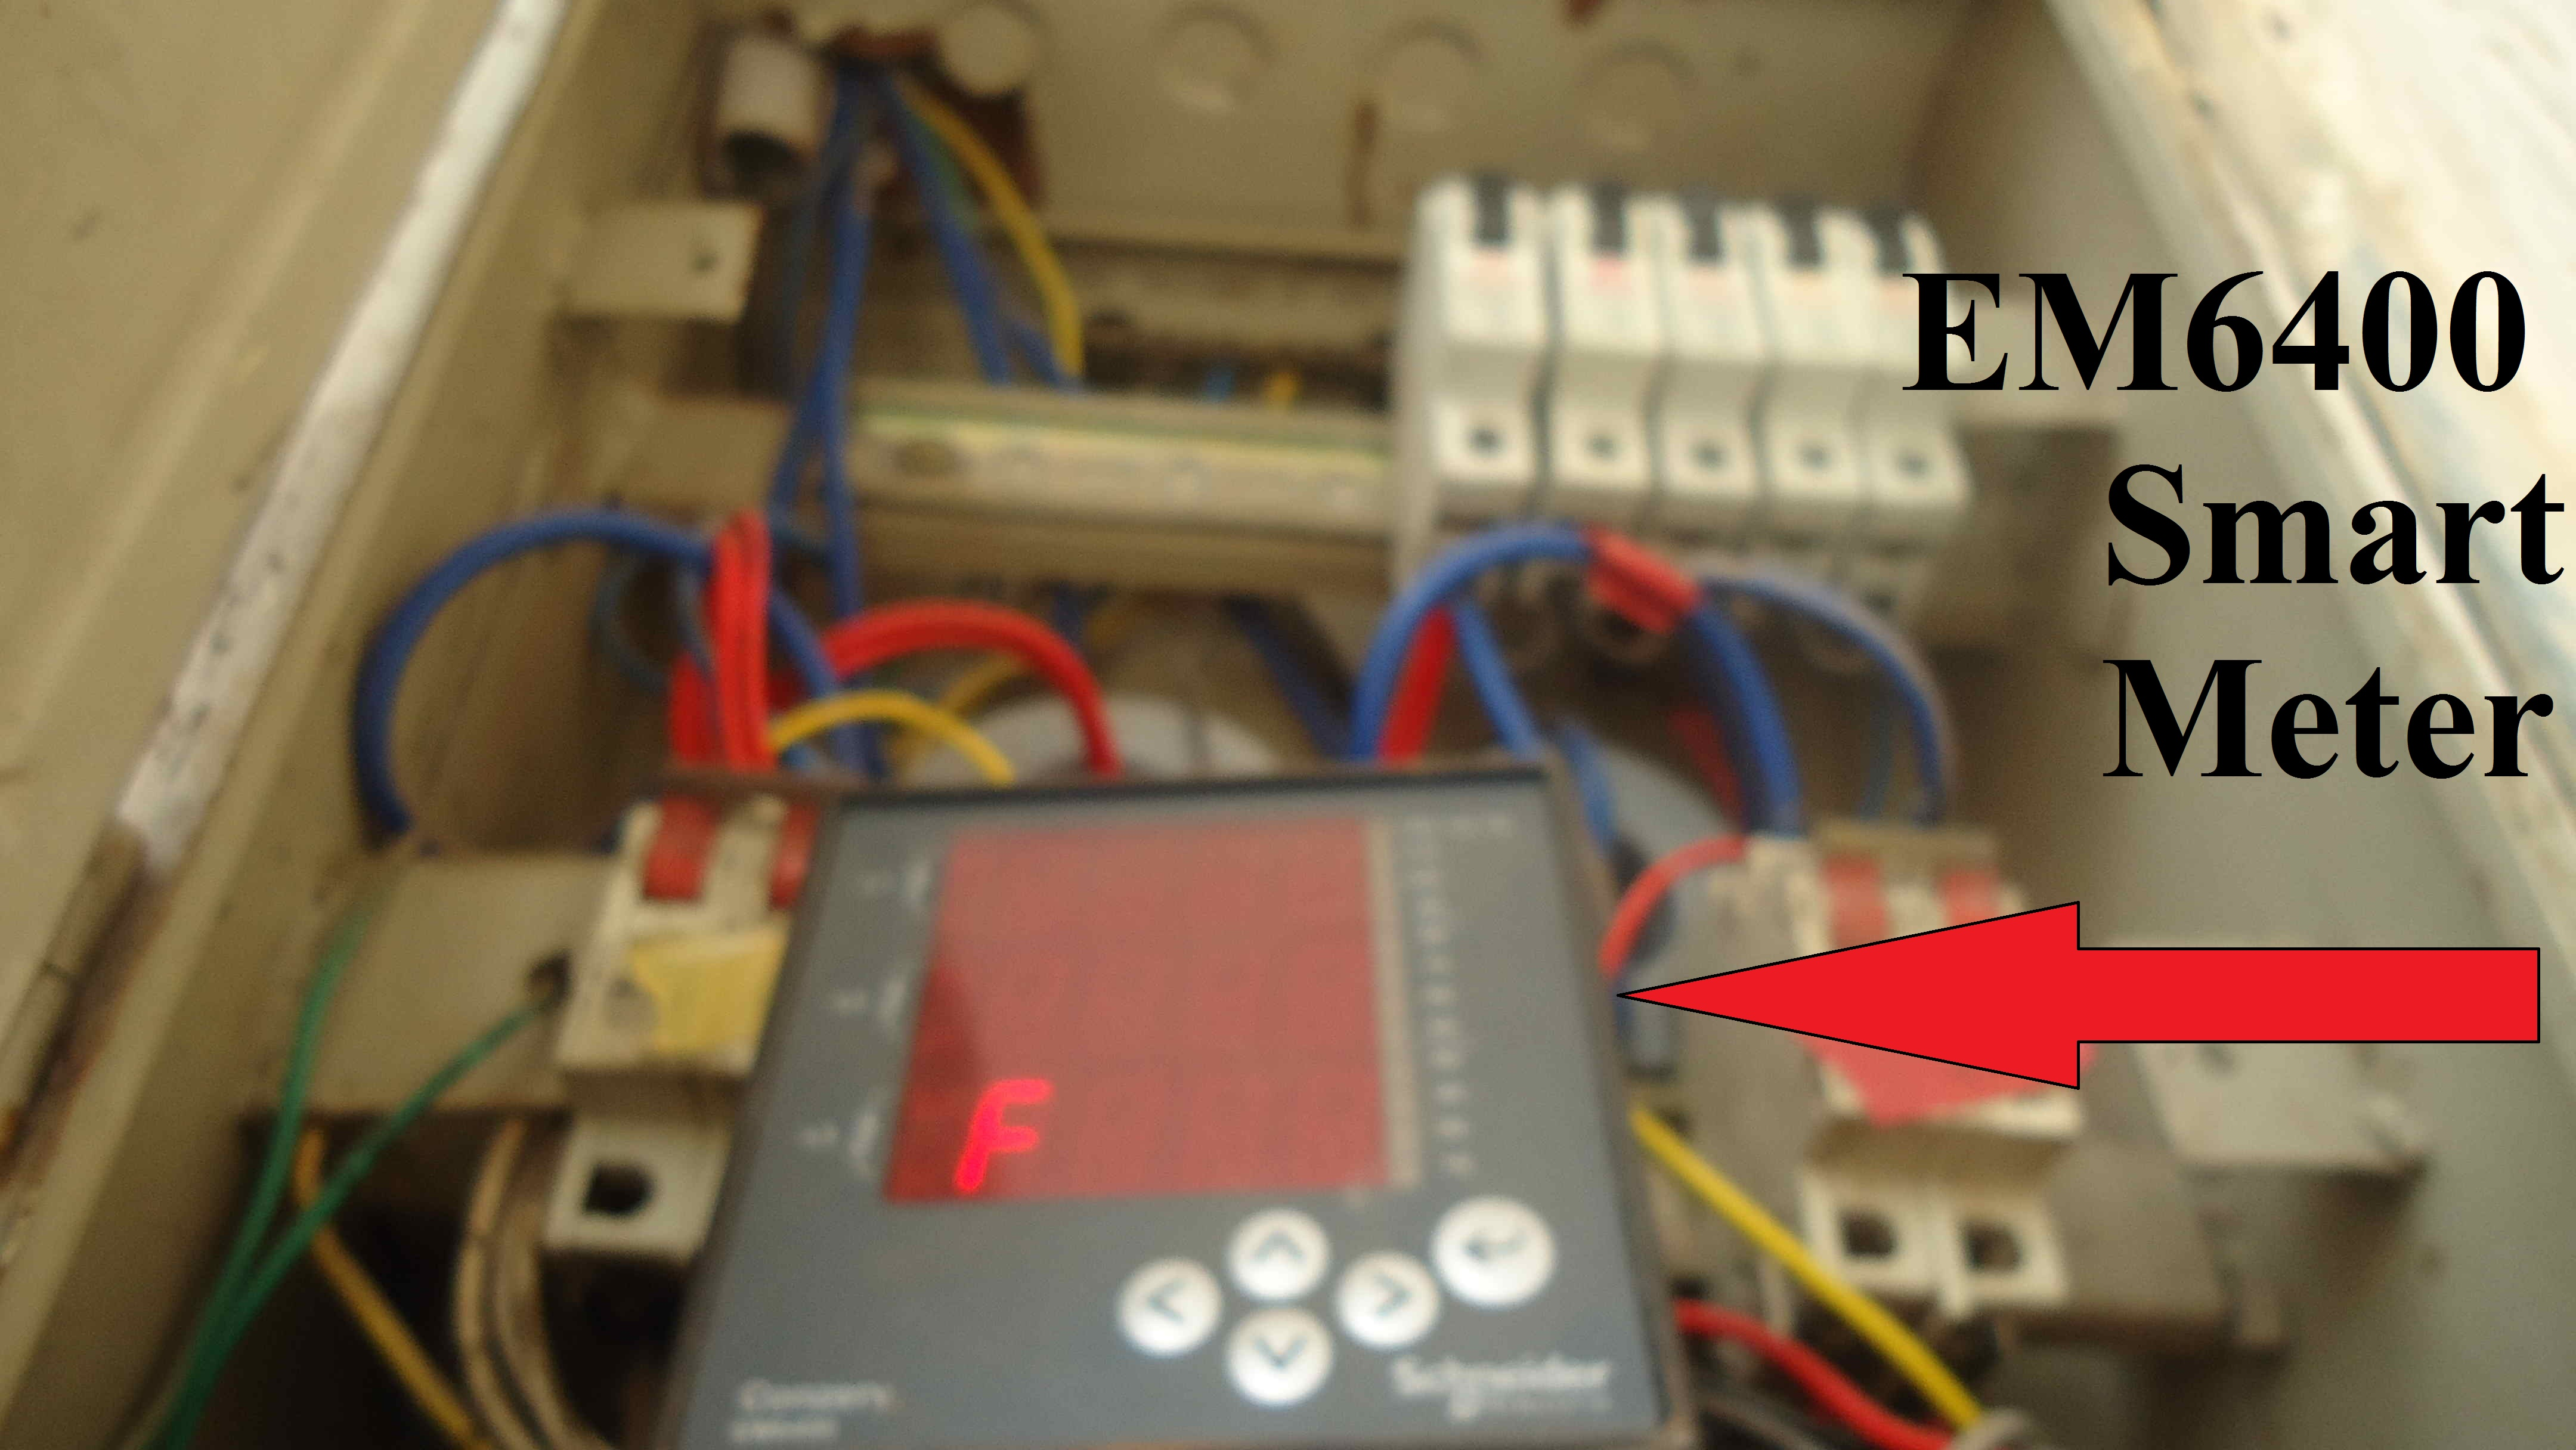
\includegraphics[scale=0.027]{./figures/electric_meter_1.jpg}}
    \hspace{1mm}
     \subfloat[\scriptsize CT based system for monitoring MCBs]{
        \label{fig:ct}
        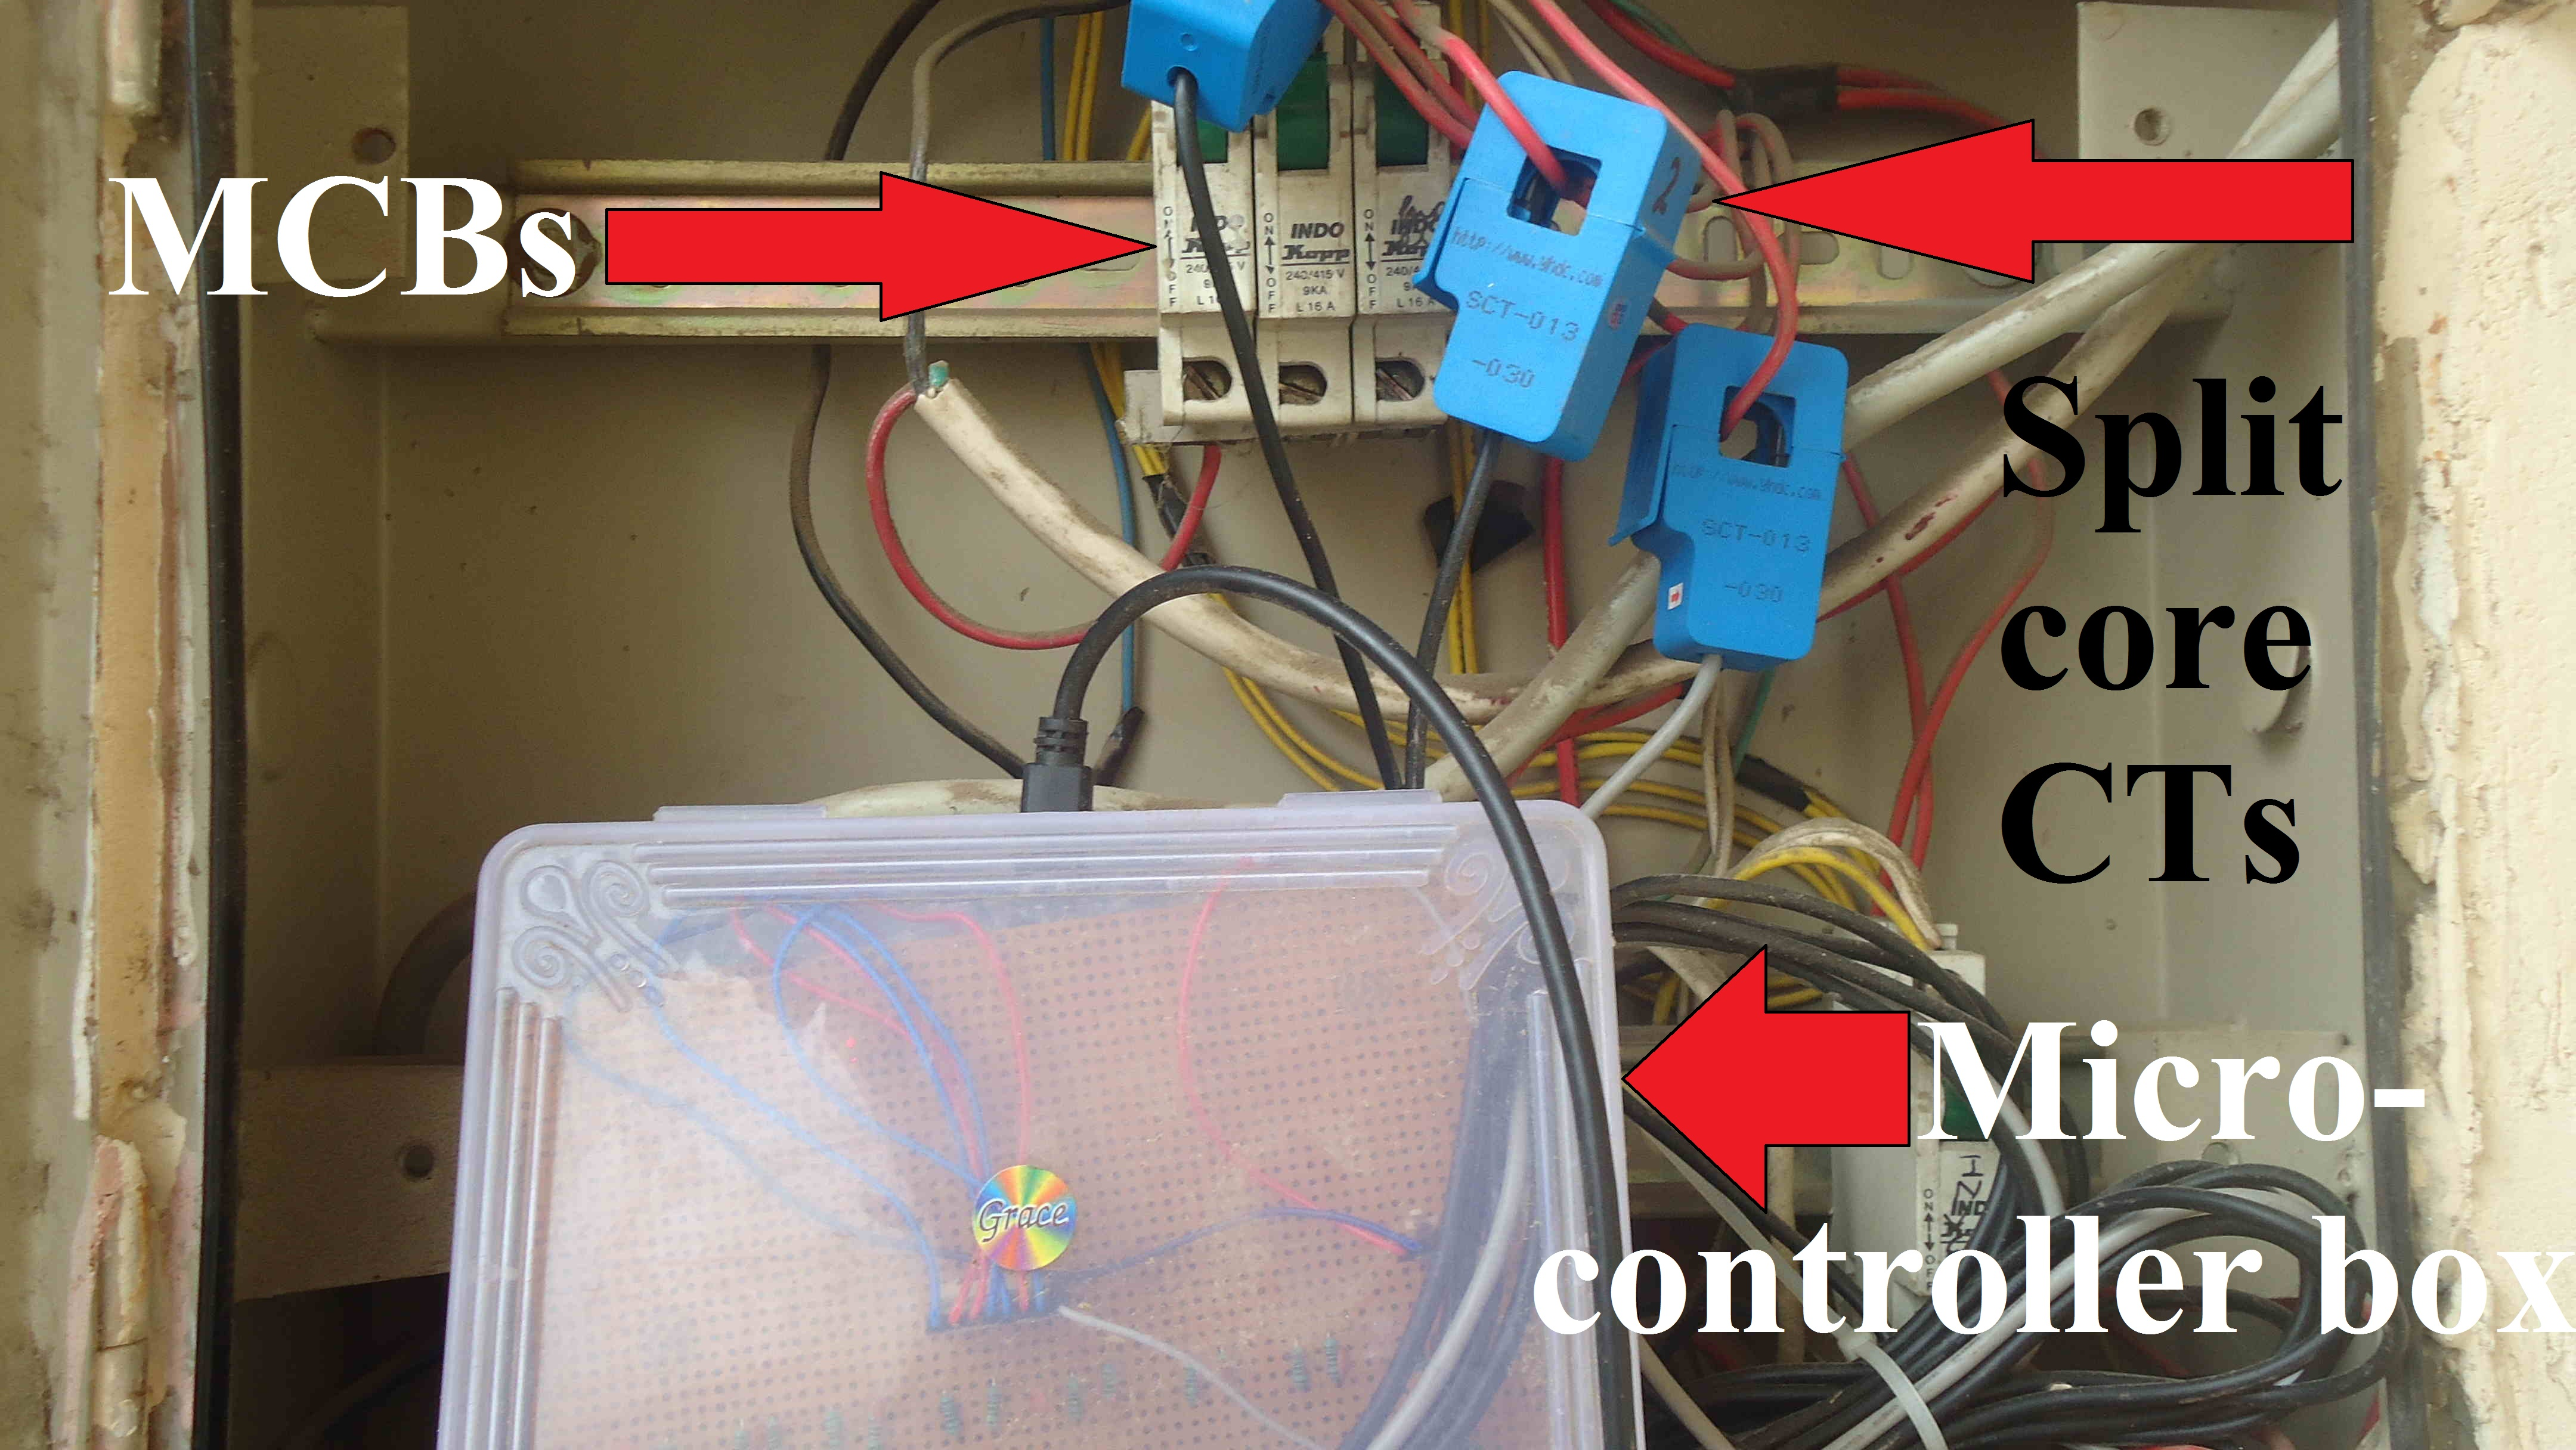
\includegraphics[scale=0.027]{./figures/mcb_2.jpg}}
       \hspace{1mm}
     \subfloat[\scriptsize Appliance level monitoring using jPlug]{
             \label{fig:jplug}
             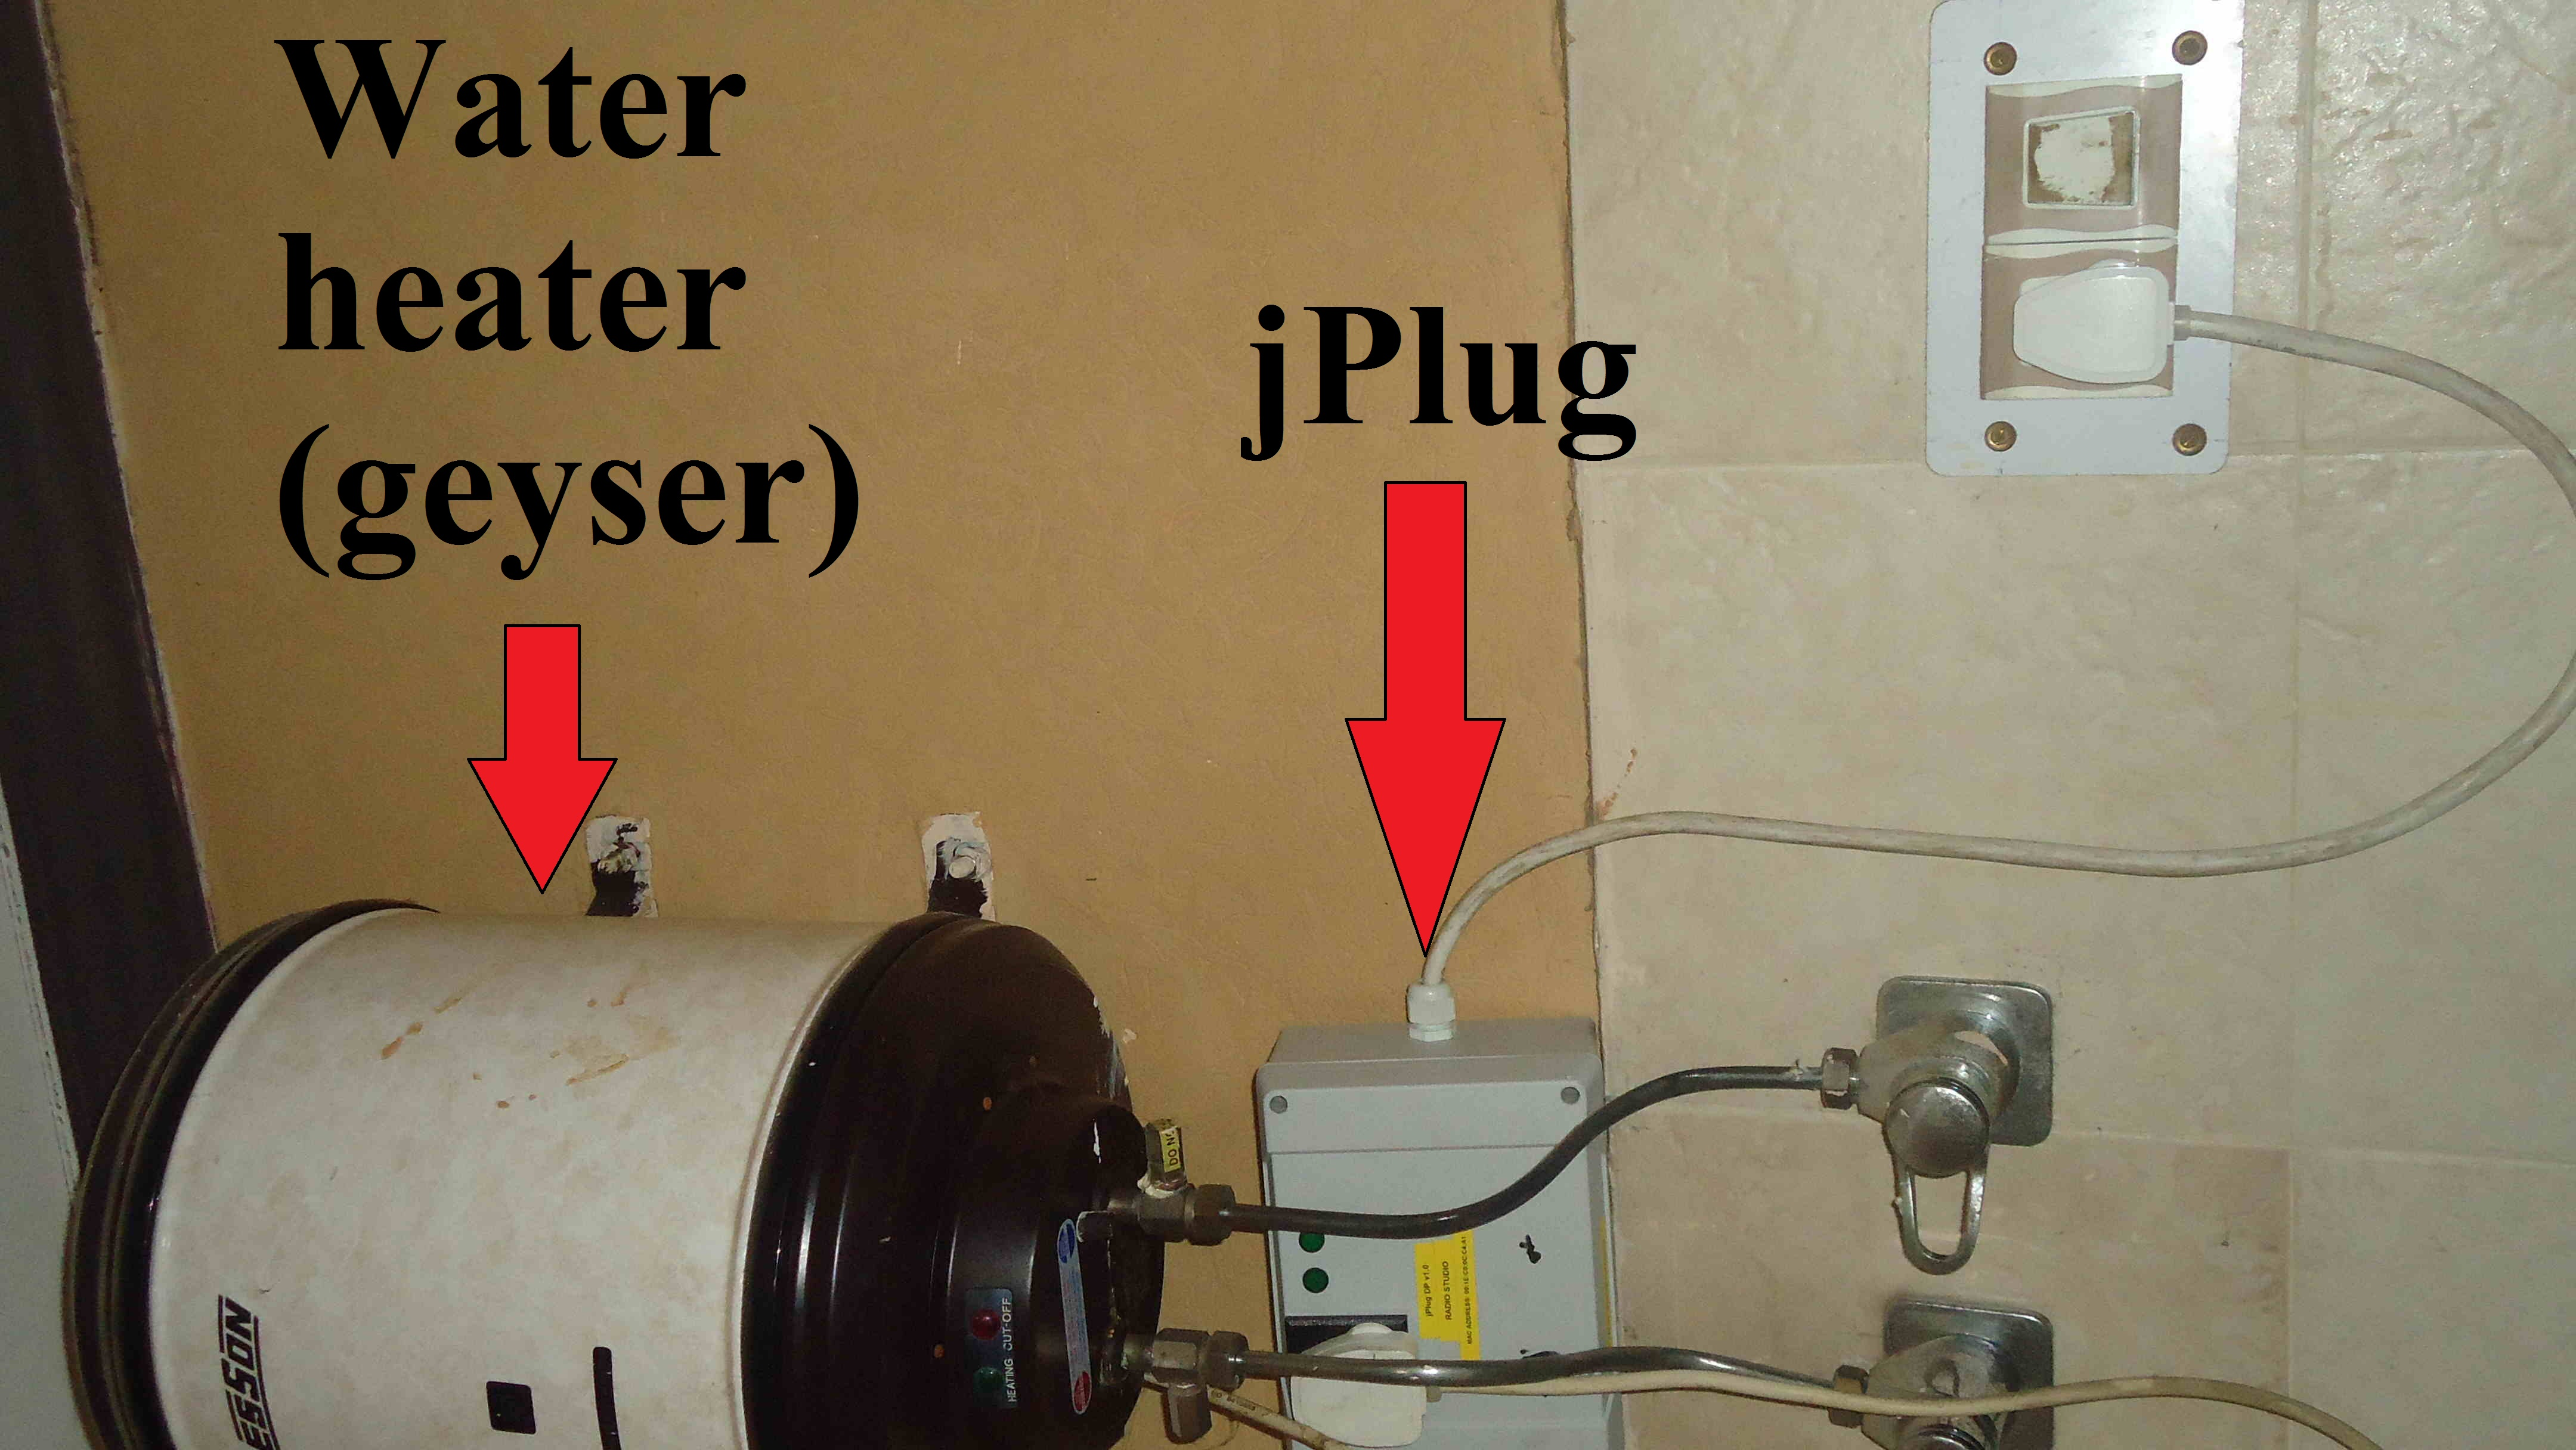
\includegraphics[scale=0.027]{./figures/jplug_2.jpg}}
             \hspace{1mm}
          \subfloat[\scriptsize Current Cost CT based monitoring]{
                  \label{fig:cc}
                  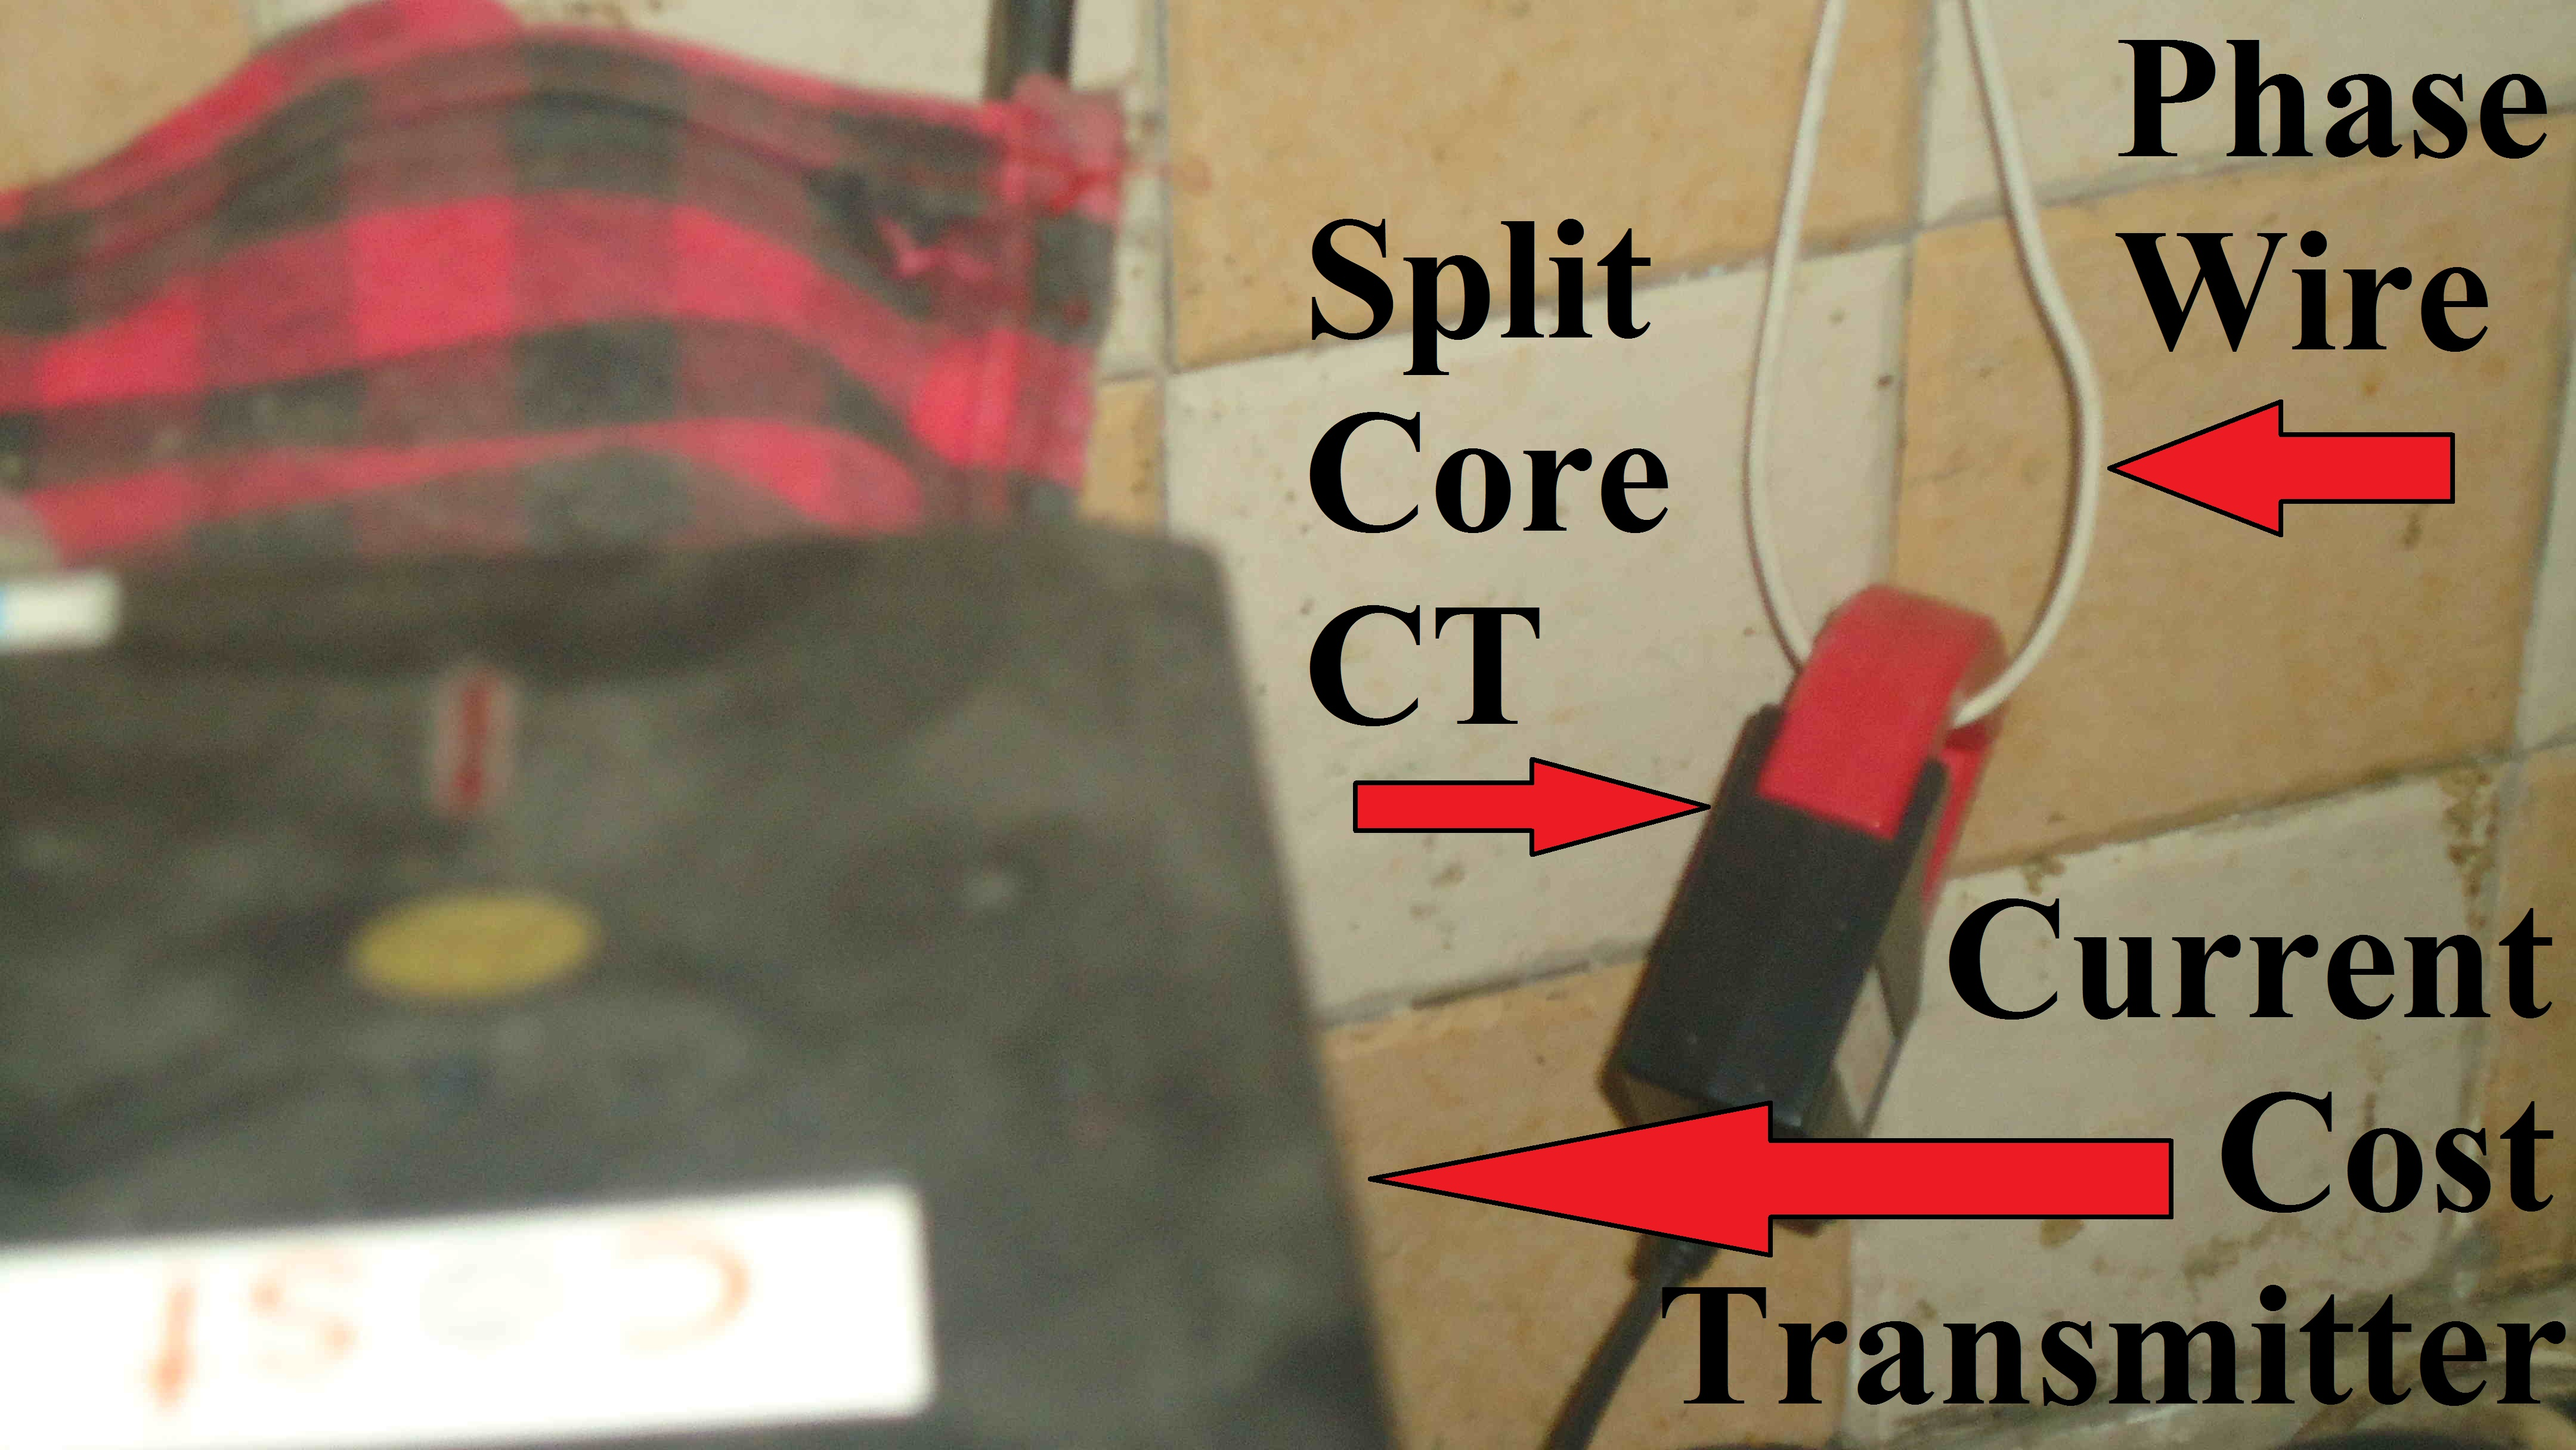
\includegraphics[scale=0.027]{./figures/cc_1.jpg}}
    %\hspace{0.02\columnwidth}
    \newline
    \vspace{-2mm}
    \subfloat[\scriptsize Water Meter]{
    \label{fig:water_meter}
        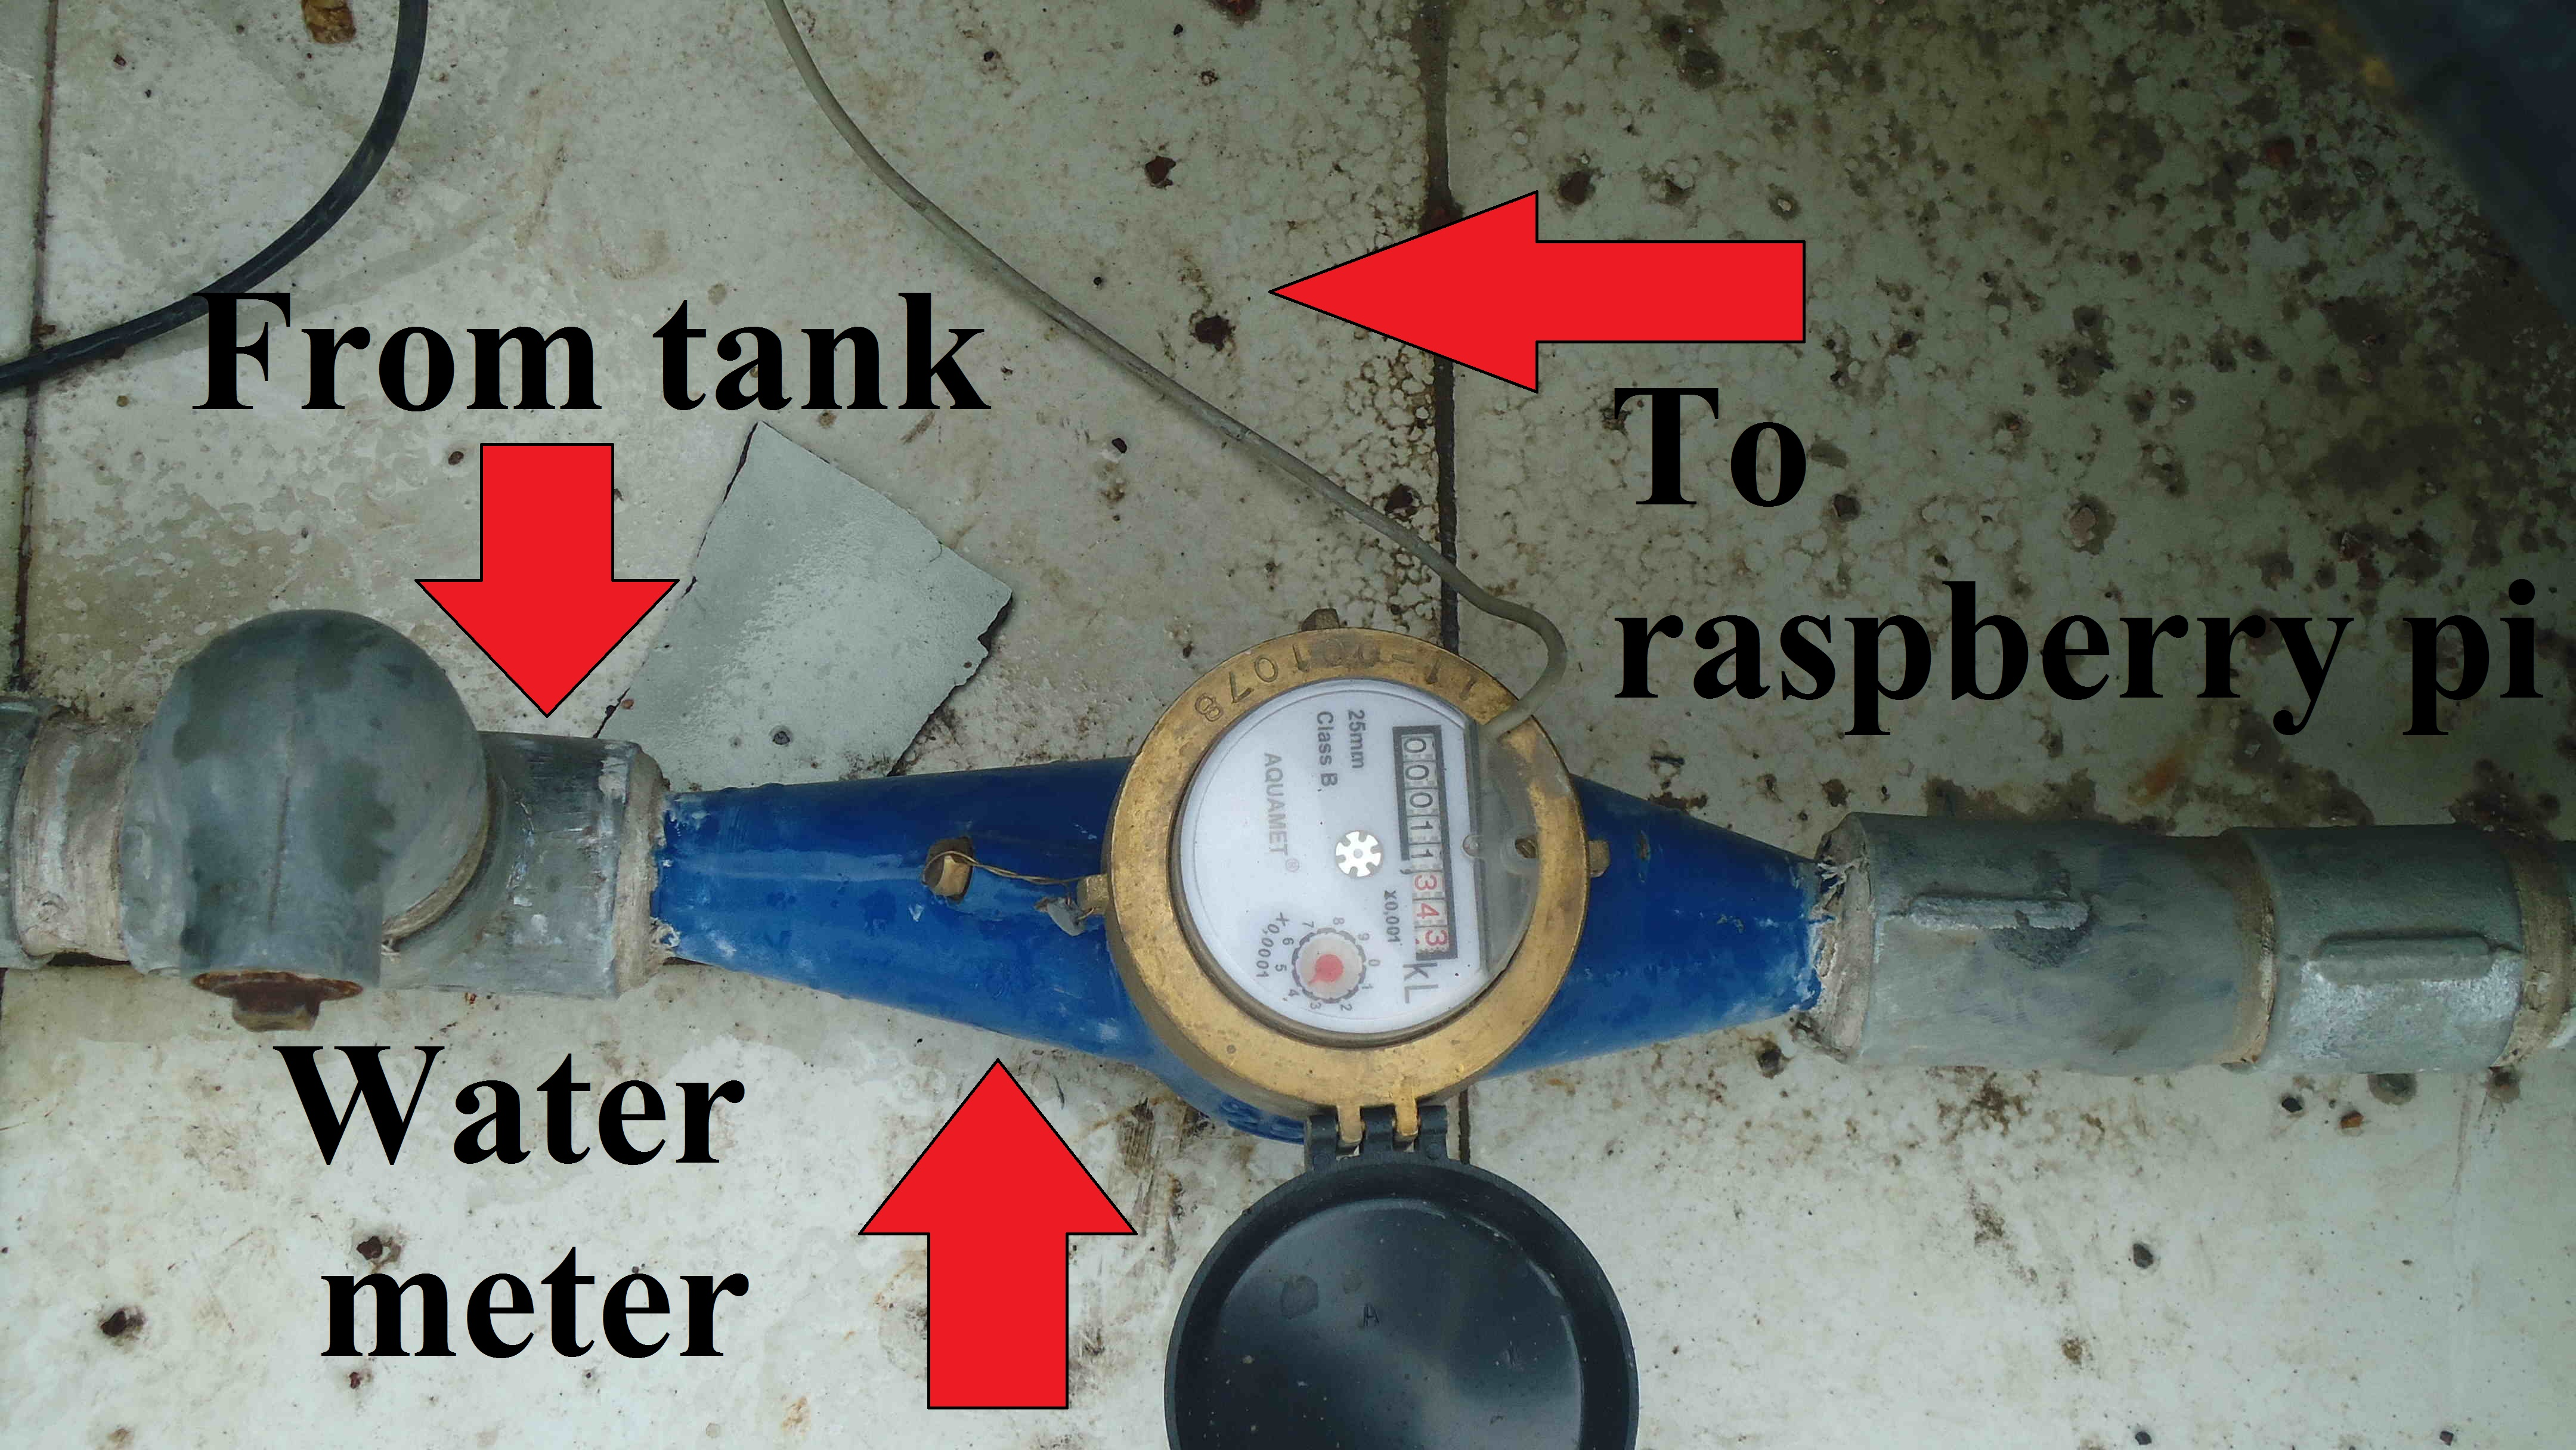
\includegraphics[scale=0.027]{./figures/water_meter_2.jpg}}
        \hspace{1mm}
        \subfloat[\scriptsize RPi collecting pulse outputs from water meter over GPIO]{
        \label{fig:rpi}
        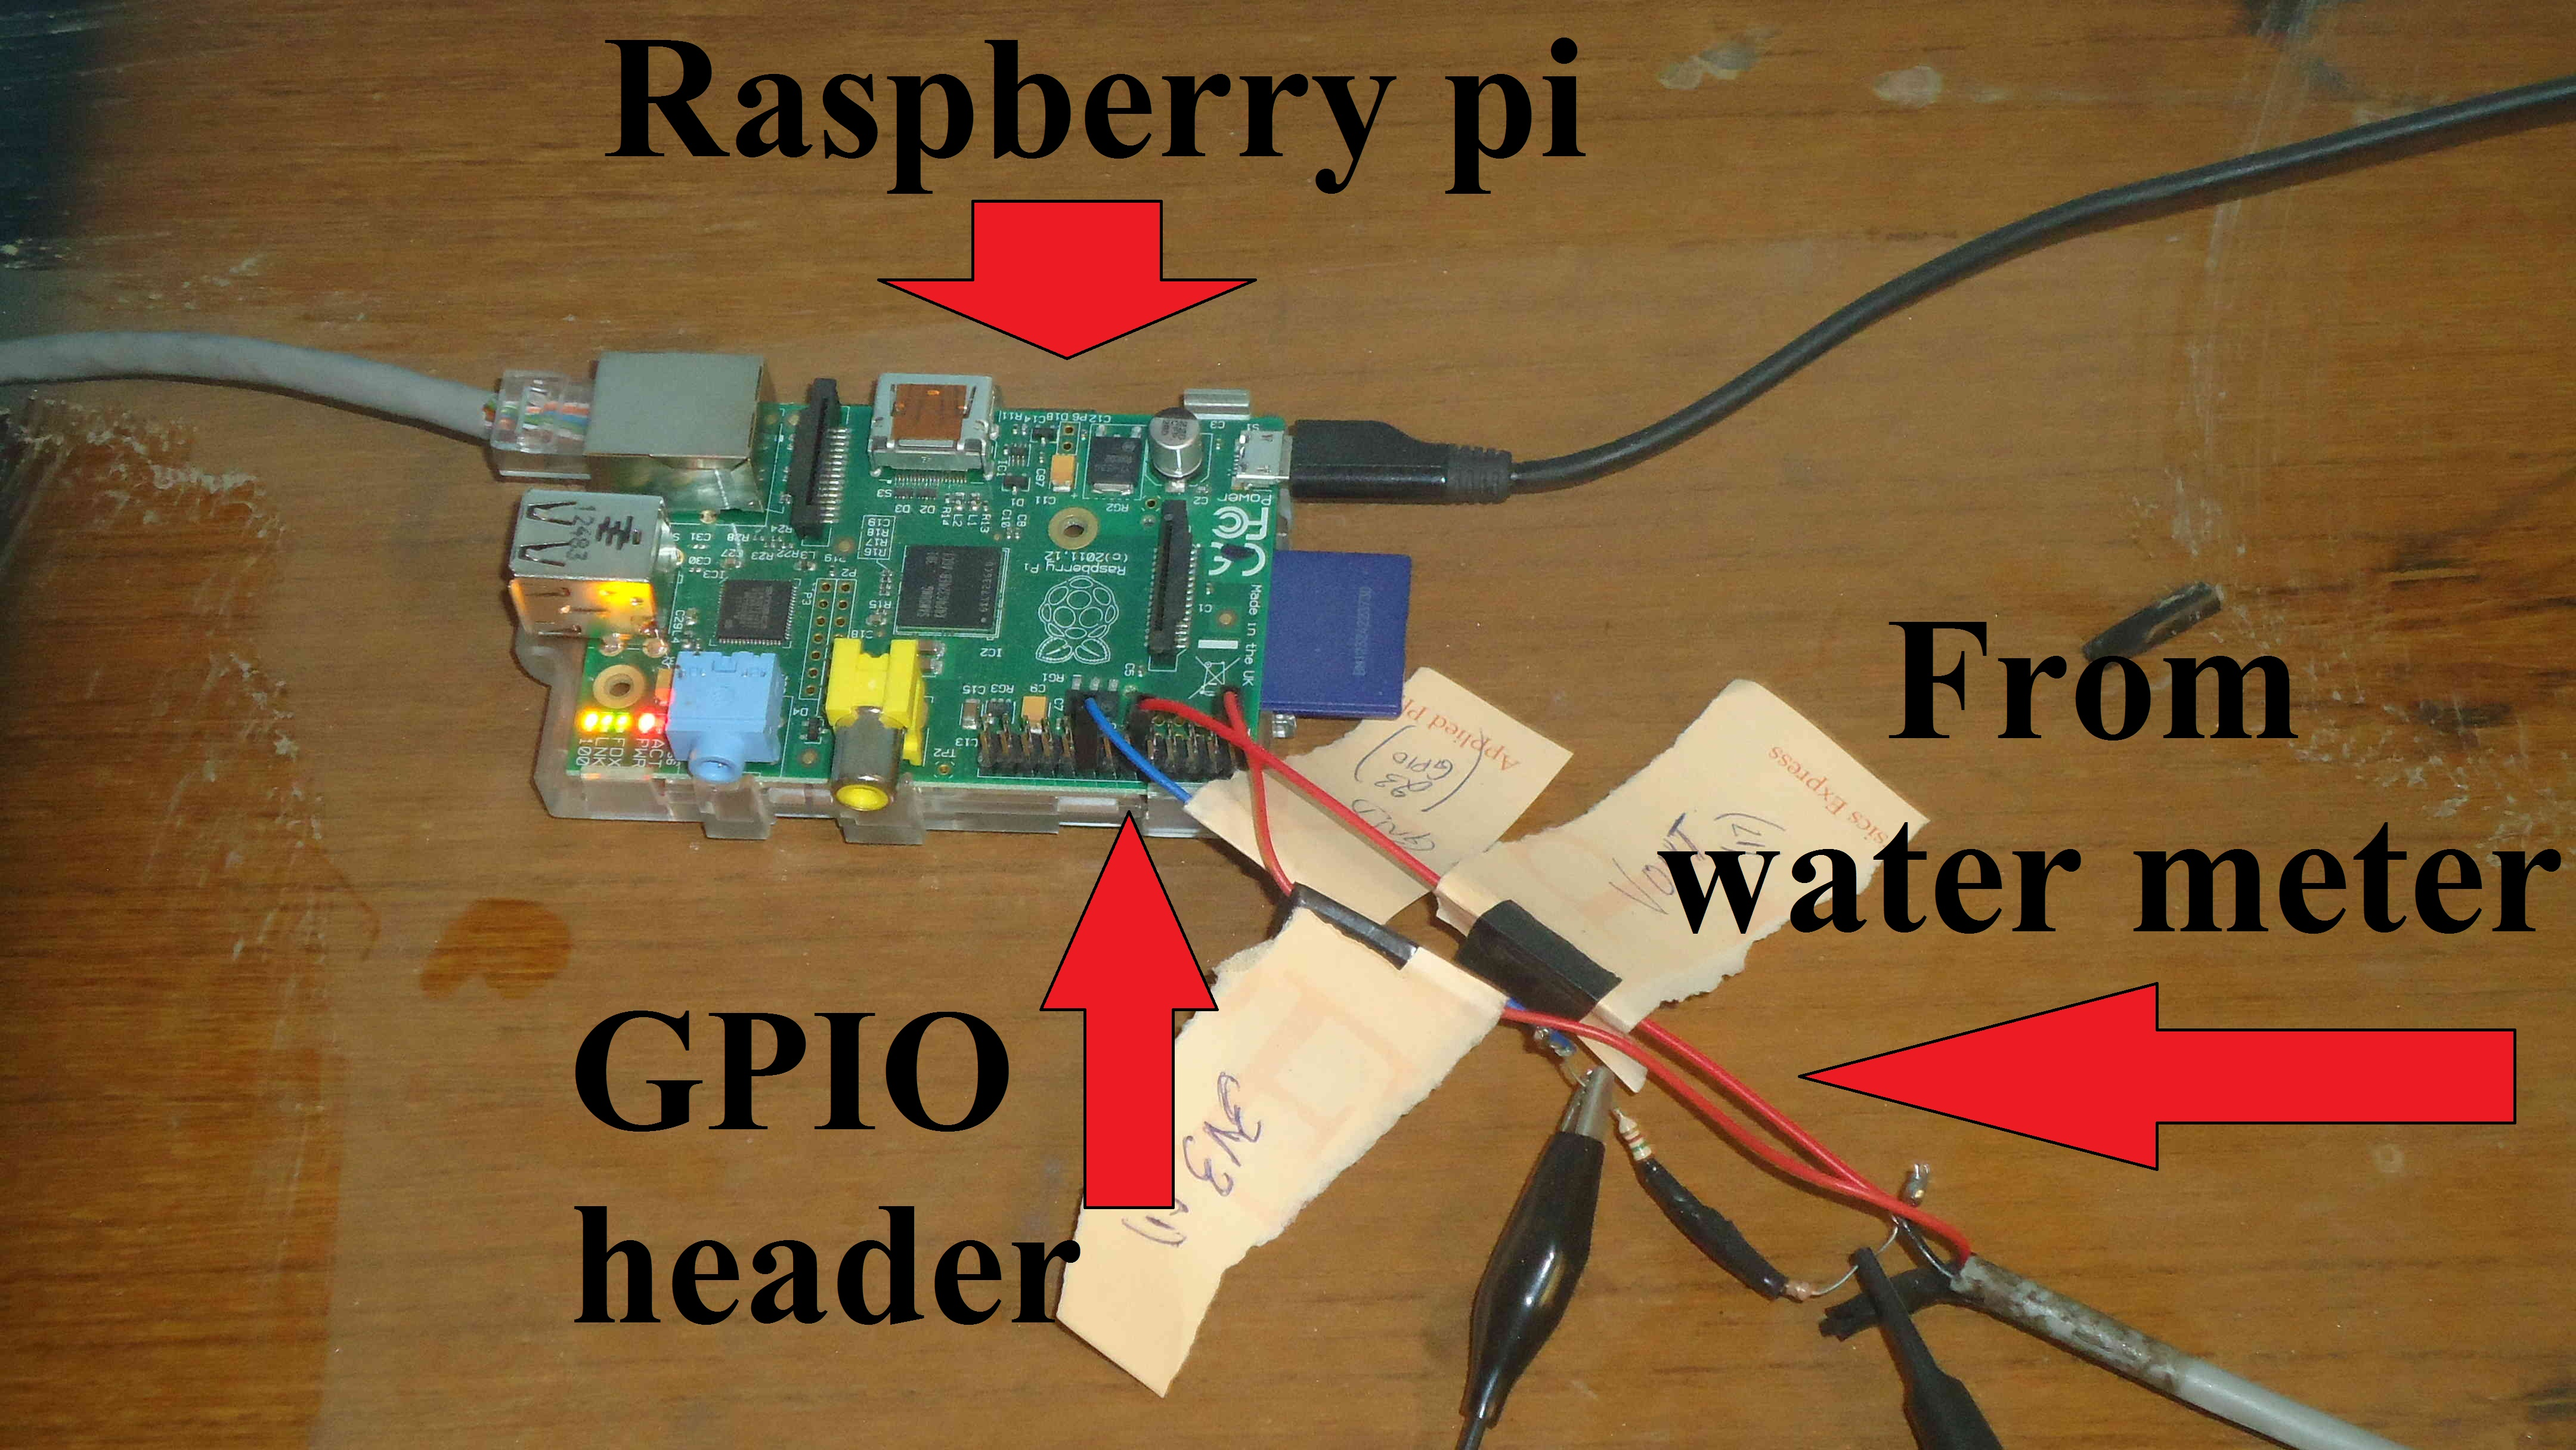
\includegraphics[scale=0.027]{./figures/rpi_2.jpg}}
        \hspace{1mm}
     \subfloat[\scriptsize Android phone and ZWave based multisensor (measuring ambient parameters)]{
        \label{fig:ambient}
            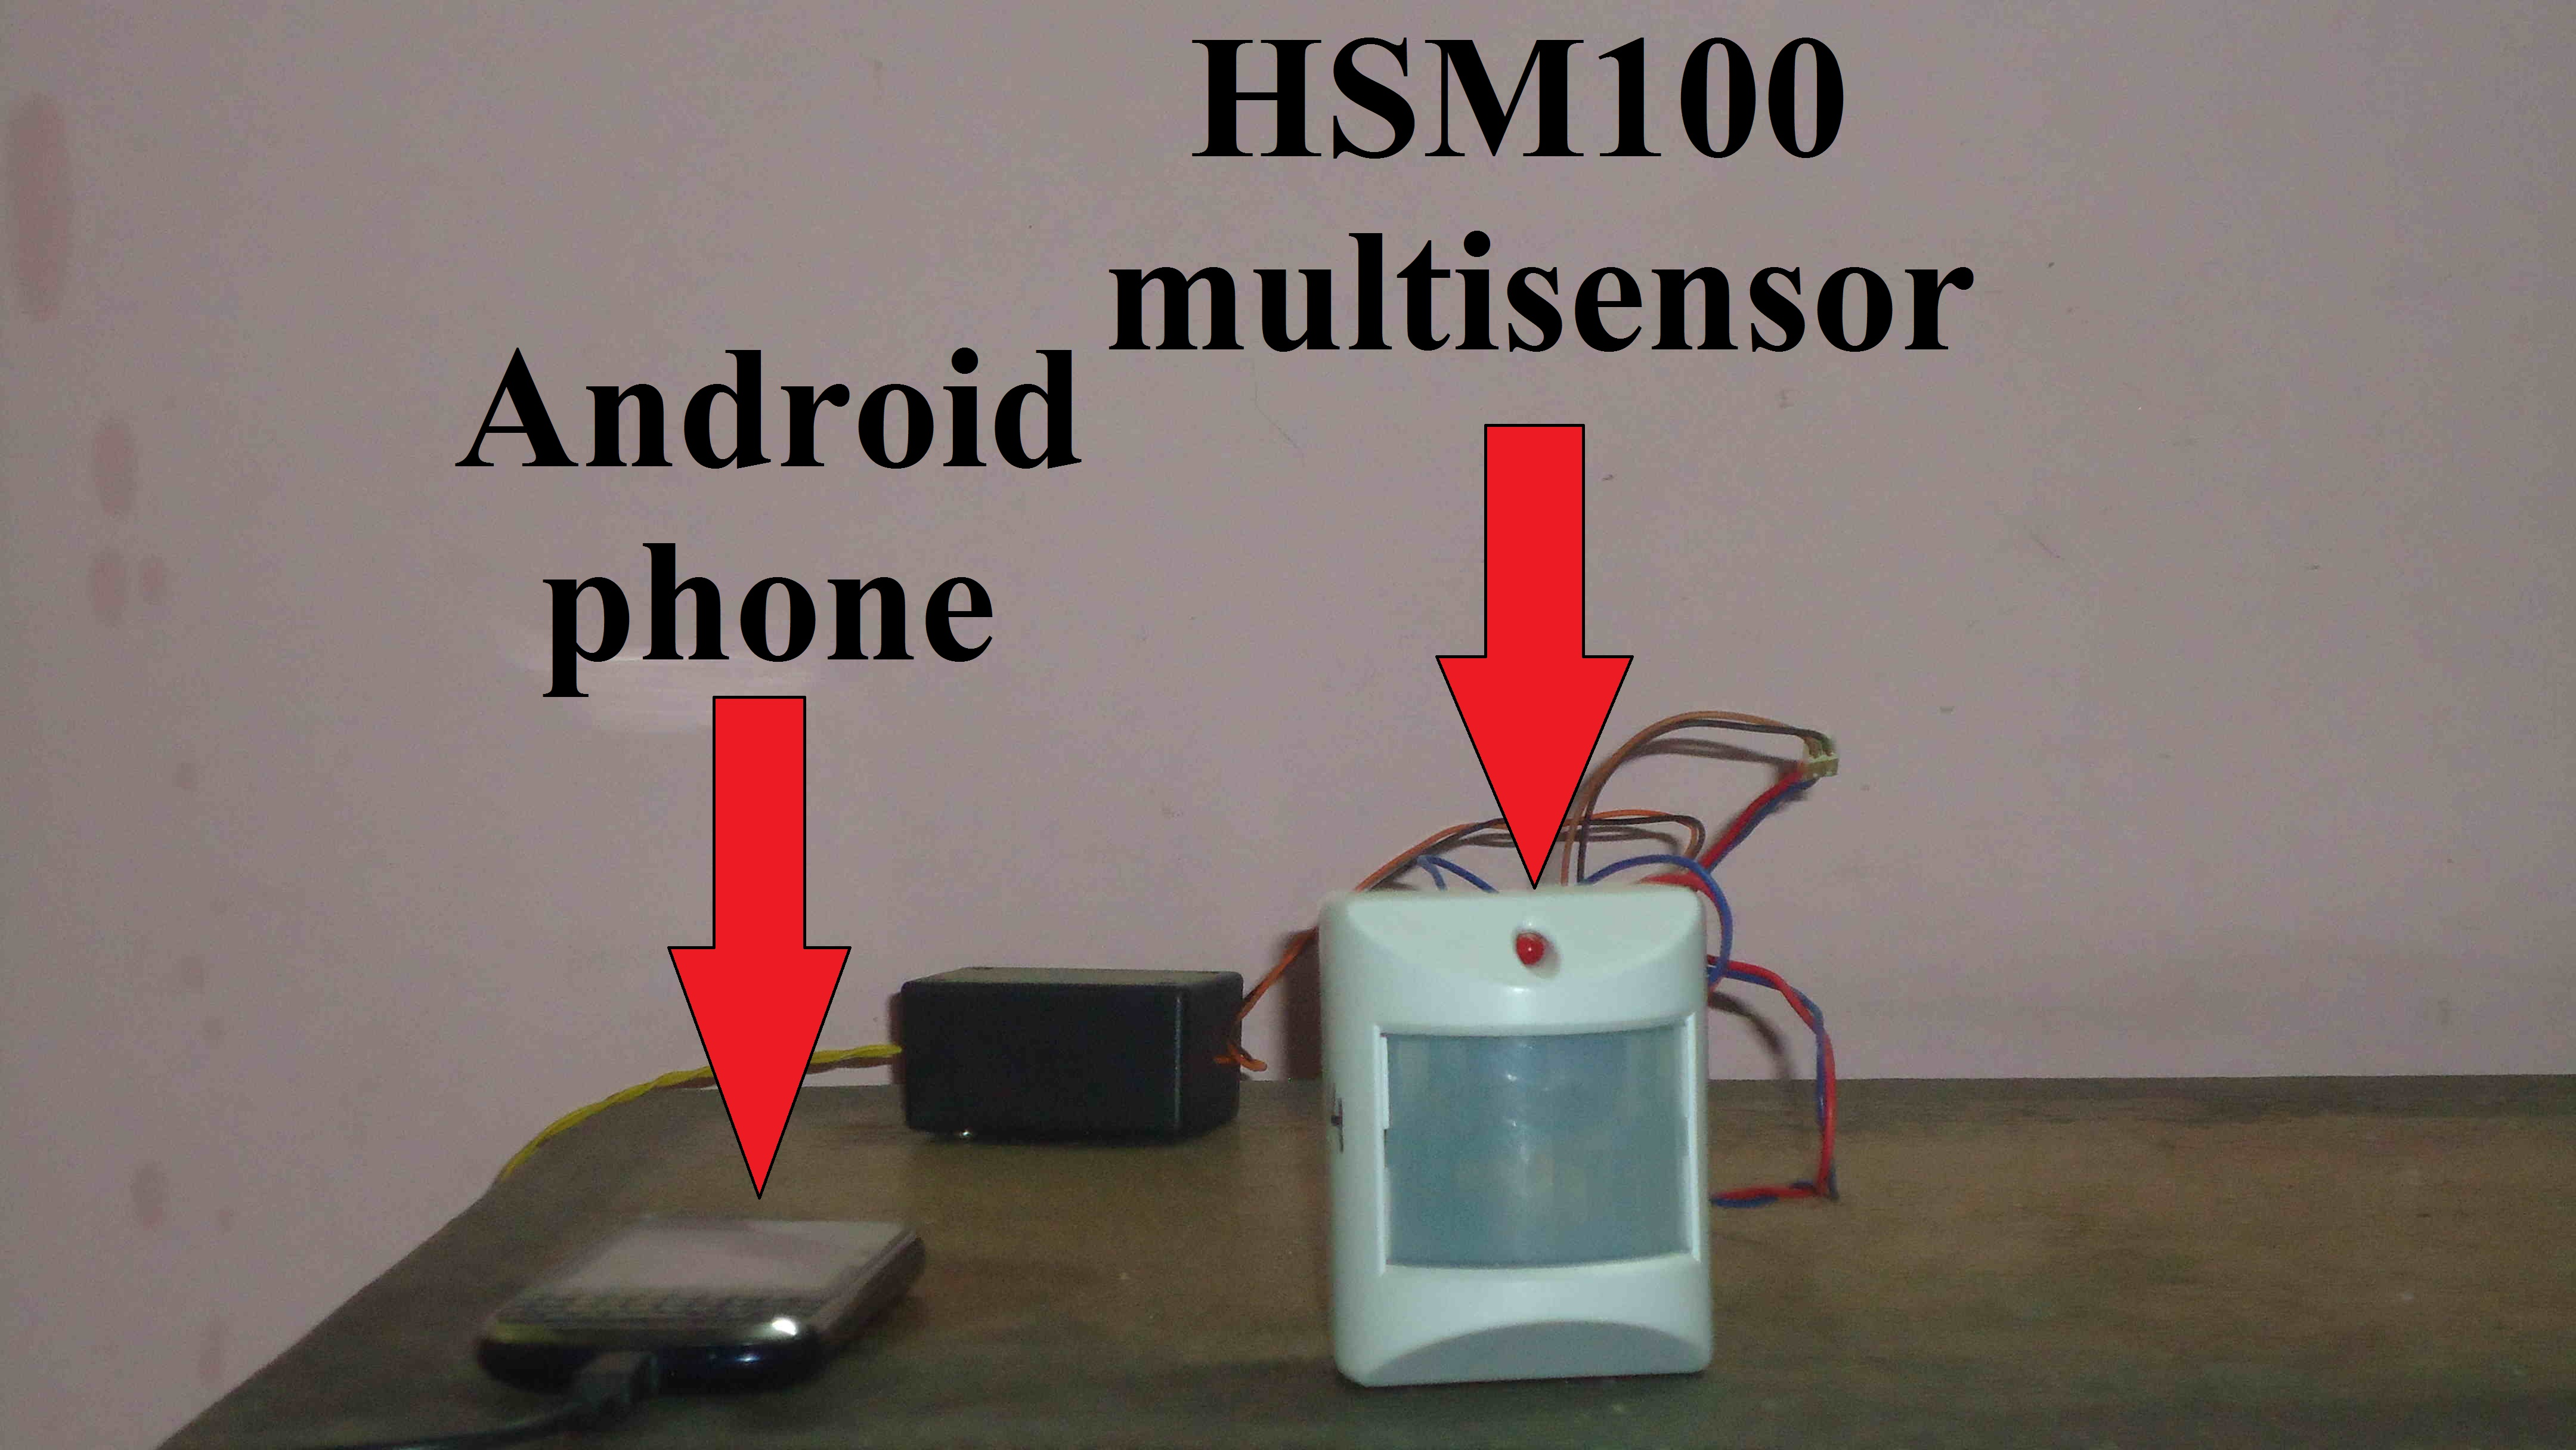
\includegraphics[scale=0.027]{./figures/ambient_2.jpg}}
            \hspace{1mm}
       \subfloat[\scriptsize Plug computer collecting ZWave data and sending over network using Ethernet]{
              \label{fig:plug}
                  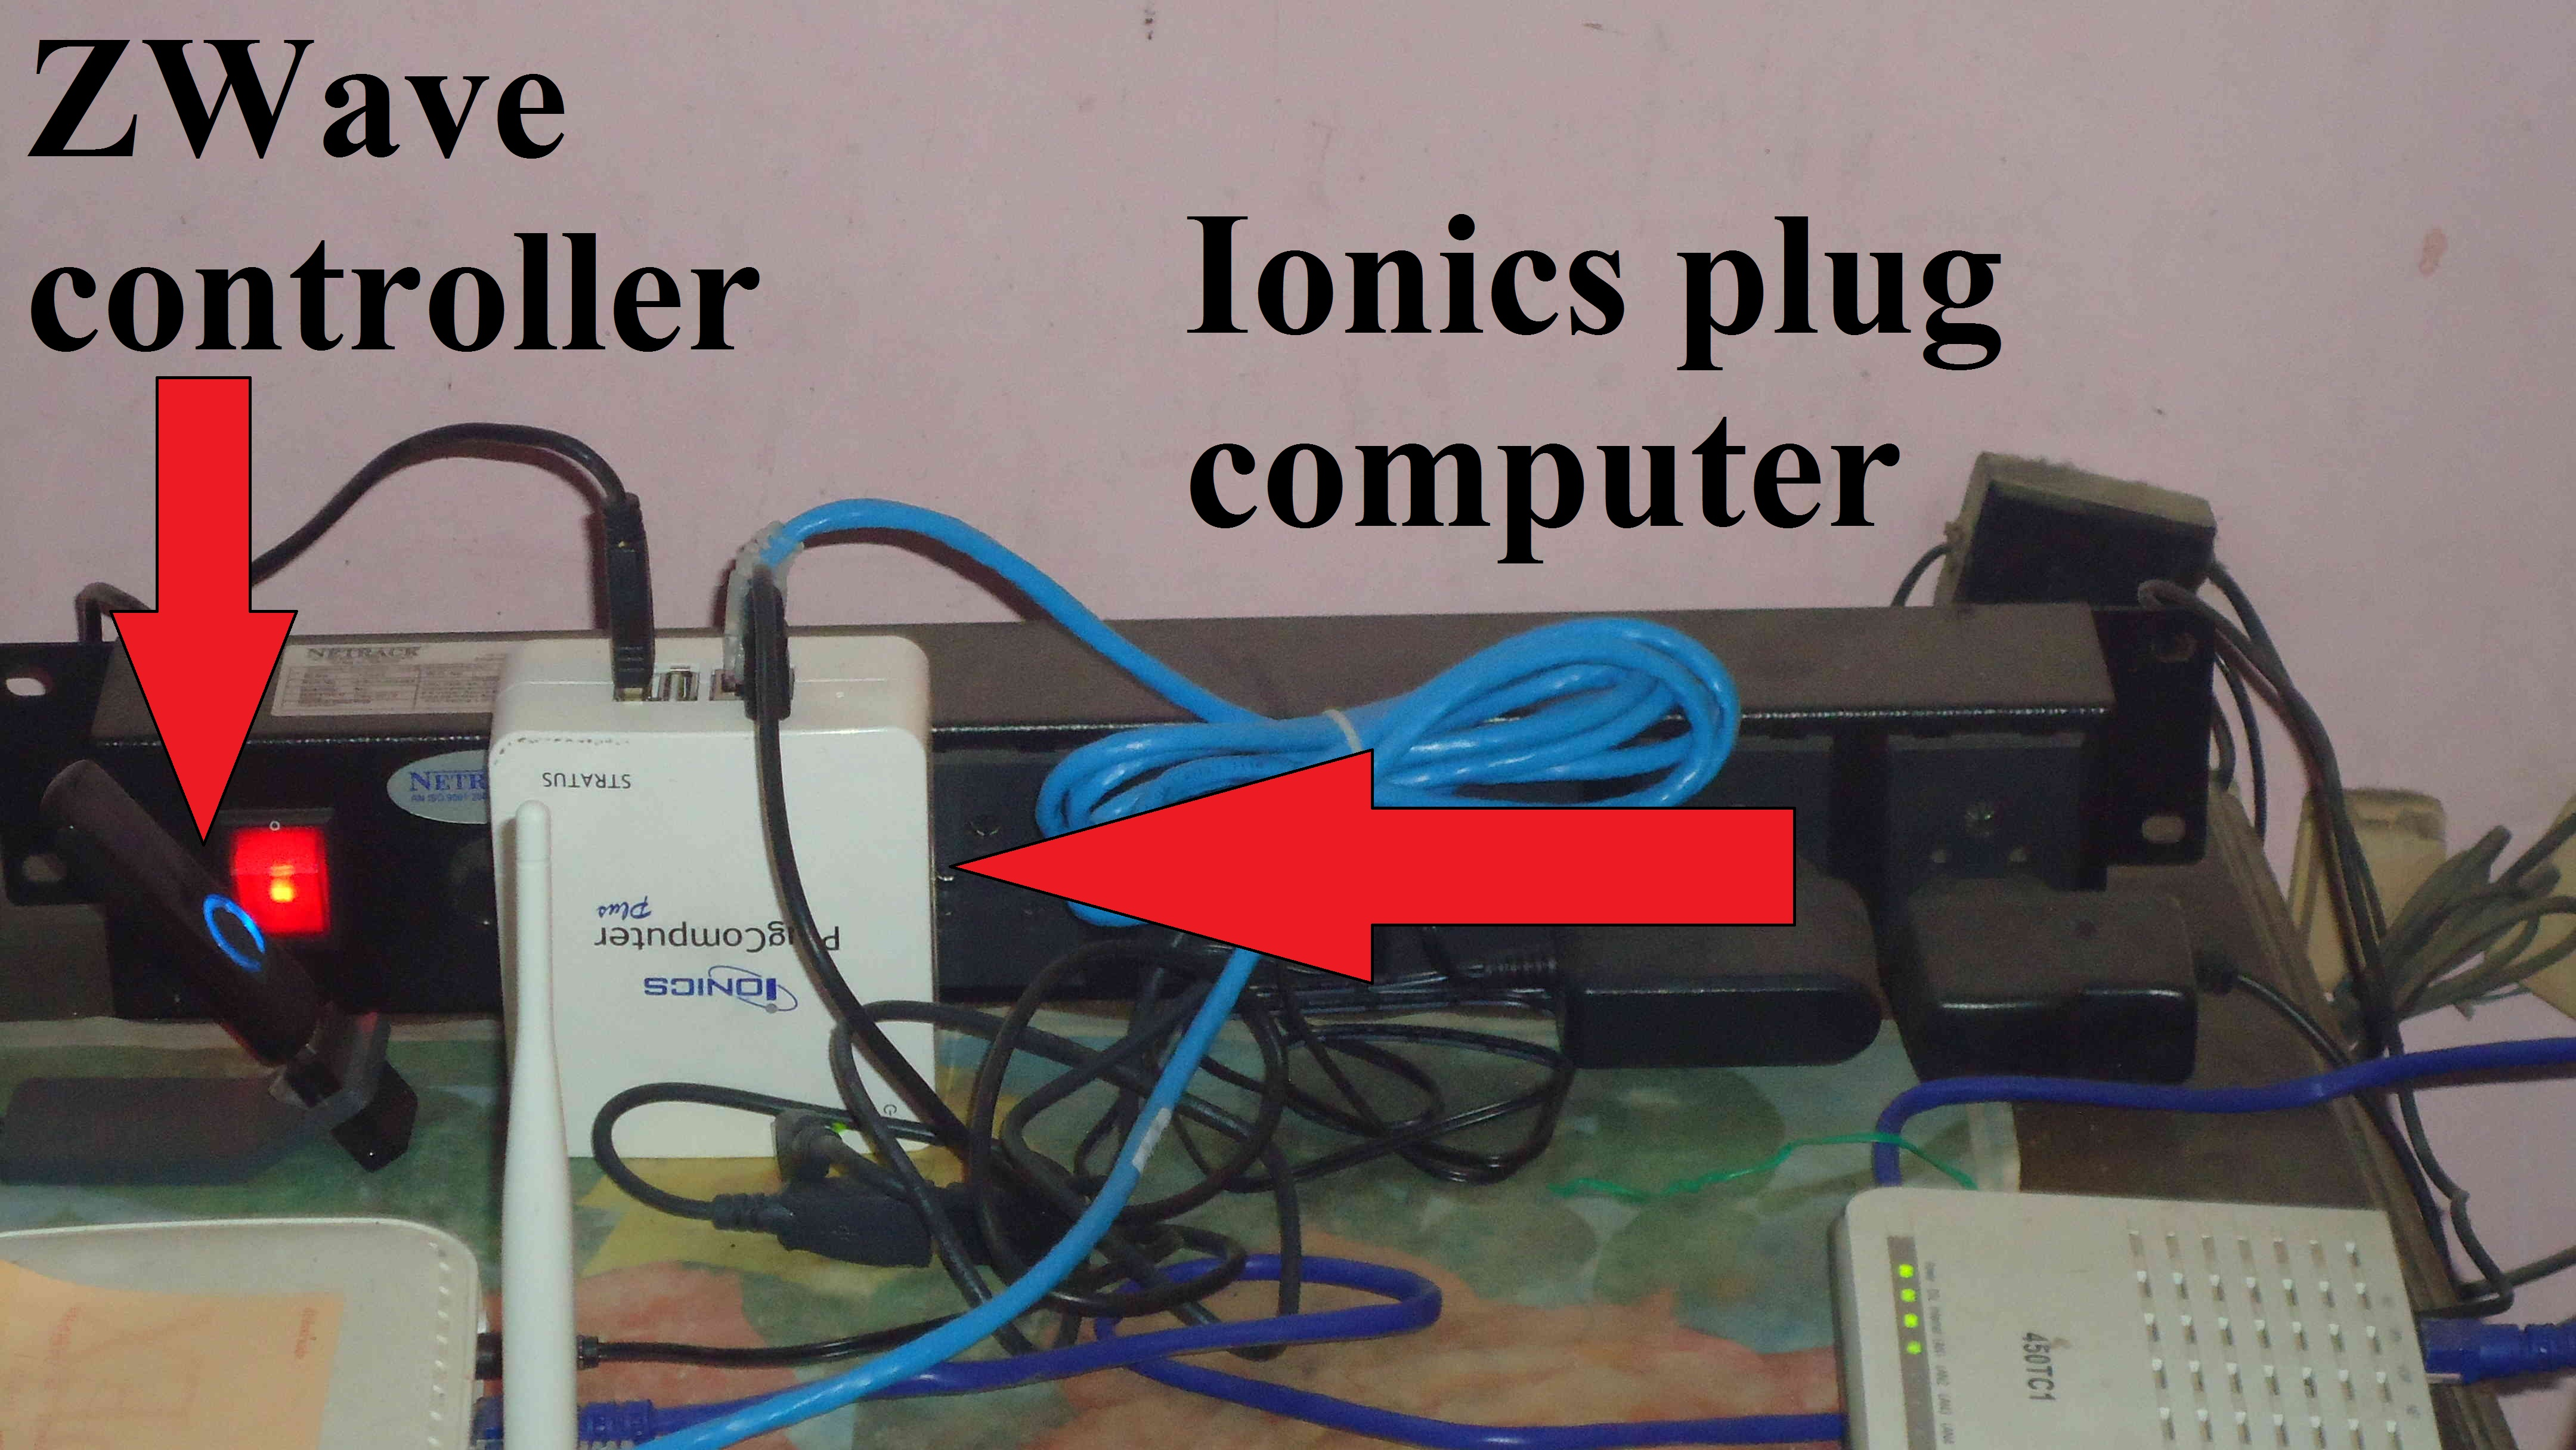
\includegraphics[scale=0.027]{./figures/plug_2.jpg}}
                 
         
	\vspace{-1mm}
    \caption{Sensing, computation and communication equipment used in our home deployment}

    \label{fig:deployment}

\end{figure*}

\begin{enumerate}[leftmargin=1em]\denselistbib
\vspace{-1.5mm}\item \looseness -2 \textbf{Meter level:} Modbus-serial enabled Schneider Electric EM6400\footnote{\url{www.goo.gl/01edPS}} meter was used to instrument the main power supply (see \figref{fig:em6400}). % showing EM6400 smart meter deployed in the electricity panel). %While cheaper variants from the same company were available, we chose to use EM6400 as it also provides reactive power. This additional information has been known to be useful for NILM applications~\cite{hart}. 
%~A 30:5 ratio CT was used on the power mains coming from the grid to ensure that the load current is transformed within the permissible limits (5 A) of the meter. 
We collected data including voltage, current, frequency, phase and power at 1 Hz. 
%The meter was deployed in March 2013 and is collecting data ever since. %through the extensive deployment phase as well. %using Modbus over RS485-serial link provided by EM6400. 
%A robust deployment was easily undertaken by a paid electrician thus demonstrating that the support required for large scale smart metering deployments exists in the Indian context. 

\vspace{-1.5mm} \item \textbf{Circuit level:} Split-core CTs, clamped to individual MCBs, are used for monitoring circuit level current. Since no commercial solution was easily available in India for panel level monitoring, we used a custom built solution involving low cost microcontroller and Single Board Computer (SBC) platform. %low cost microcontroller platform to measure current output from CTs and communicate it's RMS value over serial UART interface
\figref{fig:ct} illustrates CTs monitoring 3 MCBs on the first floor MCB box in our home. % to a single board computer. 
A total of 8 CTs were used to monitor different MCB circuits in the home.
%Since no commercial solution was easily available in India for panel level monitoring, we used a low cost microcontroller platform to measure current output from CTs at 125 KHz, calculate the RMS value and communicate it over serial UART interface (\figref{fig:ct} illustrates CTs monitoring 3 MCBs on the first floor MCB box) to a single board computer. A total of 8 CTs were used to monitor different MCB circuits in the home.

\vspace{-1.5mm} \item \textbf{Appliance level:} Since no good commercial options were available for plug level monitors, we worked with our collaborators and used their in-house developed jPlug\footnote{A variant of nPlug~\cite{nplug}} for monitoring individual appliance level power consumption. Ten jPlugs were used to monitor different plug-load based appliances across the home. 
%jPlug sits in between an appliance and the socket and provides multiple parameters (including voltage, current, phase and frequency) at 1 Hz. 
jPlug measured multiple parameters including voltage, current, phase and frequency, that were uploaded to server using HTTP POST. Additionally, Current Cost (CC) based CT is used to measure the power consumption for electric motor (used to pump water), which is not a plug-load, but has a significant power consumption (approx. 700 Watts). CC exposes apparent power data over the USB port.  jPlug and CC are shown in \figref{fig:jplug} and \figref{fig:cc} respectively.
\end{enumerate}
\begin{table*}[t!]
\footnotesize
\centering
\vspace{-4mm}
\caption{Details of sensing infrastructure used in our deployment}
\vspace{-4mm}
\label{tab:sensing}
\tabcolsep=0.015cm
\begin{center}
\begin{tabular}{|p{1.7cm}|p{2.0cm}|p{3.3cm}|p{1.5cm}|p{1.5cm}|p{2.0cm}|p{5.2cm}|}
\hline
\textbf{Sensor name} & \textbf{Procurement} & \textbf{Sampling frequency} & \textbf{Granularity} & \textbf{Quantity} & \textbf{Communication} & \textbf{Observed parameters}\\
\hline

EM6400& COTS (India)&1 Hz&Home&1&RS 485 Serial&Voltage, Current, Frequency, Phase, Power (Active, Reactive and Apparent), Energy\\ \hline
Aquamet multijet & COTS (India) &5 Hz&Main supply and tank&2&4-20 mA output to GPIO &10 liter pulse for tank output and 1 liter pulse for main supply\\ \hline
Express Controls HSM100 &COTS (Imported)&Light, temperature: 1 Hz; Motion: event based &Room &6&ZWave&Light, temperature and motion\\ \hline
Android phones &COTS (India) & Audio, light: 5 seconds every 30 seconds; Network scanning: once every 60 seconds&Room&5&Manual transfer&Audio features, light, nearby Bluetooth, cell-tower, WiFi\\ \hline
CT Monitor&Prototype &20 Hz&MCB&8&Serial&RMS Current \\\hline
jPlug& Prototype &1 Hz &Appliance&10&WiFi&Voltage, Current, Frequency, Power (Active and Apparent), Energy, Phase\\ \hline	
Current Cost&COTS (Imported)& Once every 6 seconds &Appliance&1&Serial&Apparent power\\ \hline
\end{tabular}
\end{center}
\vspace{-6mm}
\end{table*}

\begin{figure} 
\vspace{-4mm} 
\subfloat[\scriptsize Different granularity of measuring electricity consumption in home: meter, circuit and appliance]{
	 \label{fig:electricity_distribution}
    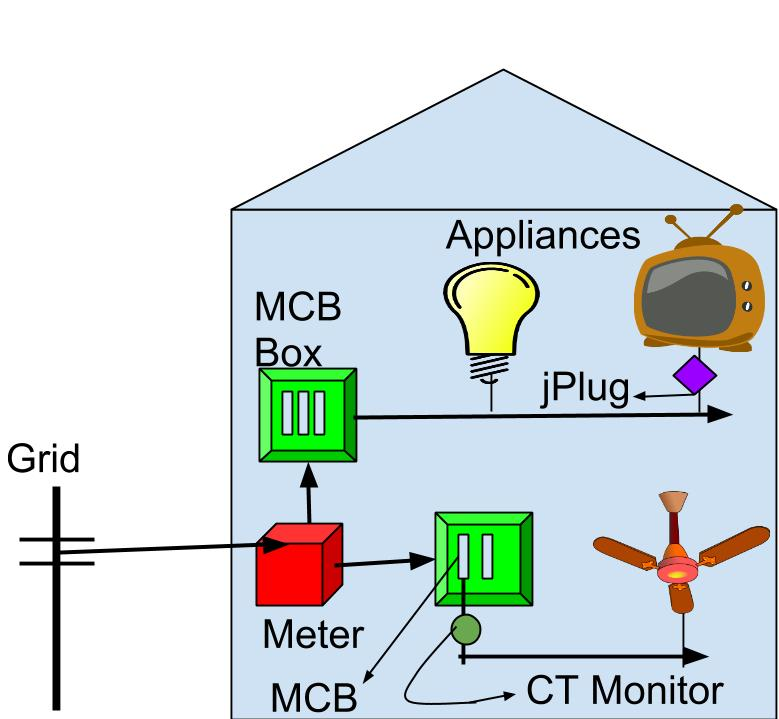
\includegraphics[scale=0.14]{./figures/electricity_distribution.jpg}}
    \hspace{1mm}
    \subfloat[\scriptsize Different granularity of measuring water consumption in home: inlet supply from utility, outlet supply from tank]{
    	 \label{fig:water_distribution}
        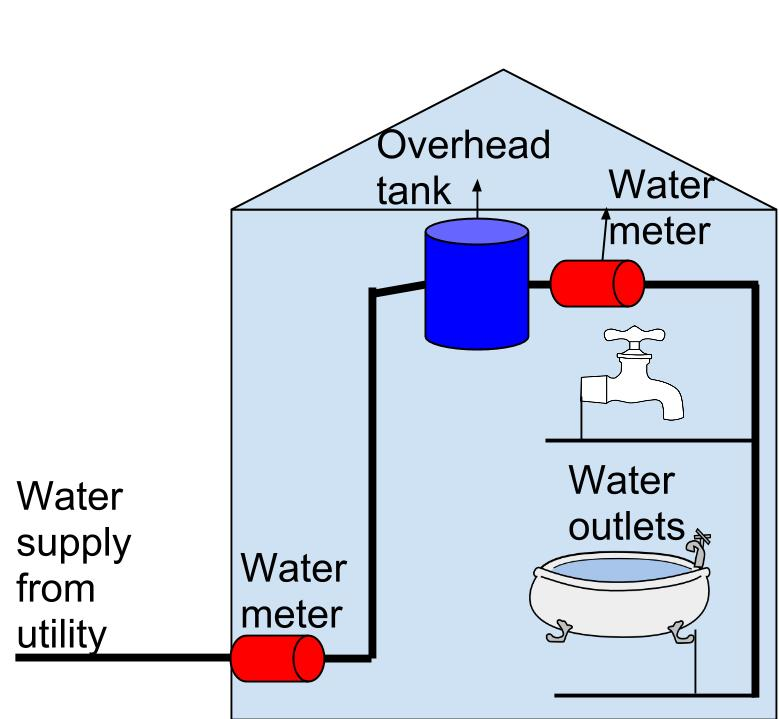
\includegraphics[scale=0.14]{./figures/water_distribution.jpg}}
        \vspace{-3mm}
   \caption{Electricity and water flow inside a home and different granularity at which these parameters can be monitored.}   
\vspace{-3mm}
\end{figure}

\noindent \textbf{Water monitoring:} 
%There are a few differences in home water distribution in India when compared to developed countries. 
To work around the short (only for a few hours a day) water supply in India, overhead water tanks (typically of 1000 liters capacity) are used to store water. Due to low water pressure, electric motors are used to pump the water for storage when the supply is available. %Thus, the flow of water in a home can be summarized as follows: 1) Water from utility comes to the home; 2) Electric motor is used to aid in pumping the water up to the tank; 3) Water flows downward from the tank whenever water is consumed. 
\figref{fig:water_distribution} illustrates the water flow distribution in the monitored home, together with the placement of water meters. One water meter is placed at the inlet (coming from the utility) and another one at the outlet from the water tank (flowing downwards). %to capture the incoming (from utility) and outgoing (from tank) water consumption. 

%Due to prohibitive cost and procurement difficulty for digital water meters in India, we chose to use Zenner Aquameter's multijet\footnote{\url{www.aquametwatermeters.com/multijet.html}}. 
Due to prohibitive cost for digital water meters in India, we chose to use Zenner Aquameter's multijet\footnote{\url{www.aquametwatermeters.com/multijet.html}}. The multijet uses pulse output generated through a 4-20 mA current loop. 
%Pulse output is commonly used for analog signaling in industrial process control instruments. 
Water meter connected to the utility, over a 0.5 inch diameter pipe, generates a pulse for every 1 liter of water consumption. Water meter connected to the outlet of storage tank, with 1.25 inch diameter, generates a pulse every 10 liters of water consumption. %generating a pulse every few liters. The precision is based on the quality of the sensor and the diameter of the water pipe. The water meter we used for overhead tank gives a pulse every 10 liters, whereas the one used for inlet supply from utility gives a pulse every 1 liter. These pulses can be measured using the circuit diagram for 4 ma loop shown in ... 
\figref{fig:water_meter} shows the water meter deployed inline at the overhead tank.

\noindent \textbf{Ambient monitoring:} ZWave based Express Controls HSM100\footnote{\url{http://goo.gl/Bszg0u}} multisensors were used for monitoring motion, light and temperature across 5 rooms in the home. To the best of our knowledge, no commercial ZWave based sensor is available that works on Indian frequency (865.2 MHz). We correspondingly imported EU frequency (868.4 MHz) devices and used them for ambient monitoring. For these HSM100, motion is reported in an event-driven manner (i.e. whenever there is change in motion status, a reading is reported) and temperature and light are polled at 1 Hz. An Android phone, running FunF journal application\footnote{\url{http://www.funf.org/journal.html}}, was placed at a fixed location in each room to log ambient parameters such as light and sound level every 30 seconds for 5 seconds.

\noindent \textbf{Miscellaneous:} Android phones, in addition to measuring ambient conditions, were also used to scan and log Bluetooth, WiFi and GSM networks. All the home occupants were requested to keep the Bluetooth, for their personal phone, on during the duration of the experiment. The network scanning was done every 1 minute and is stored locally on the SD card. External weather conditions, such as temperature, humidity and wind speed, were also logged every 10 minutes using publicly available APIs from weather monitoring stations\footnote{Forecast, World Weather, Open Weather Map}.
%\footnote{Forecast: \url{www.forecast.io}, World Weather: \url{www.worldweatheronline.com}, Open Weather Map: \url{www.openweathermap.org}}
%Additionally, network traffic was sensed to monitor connectivity and signal strength.

%Such miscellaneous data collection, together with detailed electrical consumption, water consumption and ambient information, can be used for multiple applications including energy-apportionment (i.e. assigning energy usage to different occupants within the home), localization and correlating energy usage with outside temperature.

Complete sensing infrastructure, used in our deployment, is summarized in \tabref{tab:sensing}.

\vspace{-1mm}
\subsection{Communication and Computation}
\label{sec:comm_comp}
%Our sensing infrastructure, described in \secref{sec:sensing}, involves multitude of communication channels. 
Different computing platforms - microcontrollers, SBCs and desktops are used for data collection.  
%In our experience we found that using a desktop computer for collecting data from individual sensors would be an overkill in terms of cost, processing power and physical space used. Although microcontrollers are cheap and occupy little space, they do not expose enough abstractions for high level programming, are often difficult to debug and are inherently hard to multi task. We thus decided to use Single Board Computers (SBC's) for sensor data collection. We used Raspberry Pi\footnote{\url{www.raspberrypi.org}} (RPi) and Ionics Stratus\footnote{\url{www.ionics-ems.com/plugtop/stratus.html}} based SBC's. 
%SBCs served as a good low cost alternative (25 \$) constituting 700 MHz ARM processors and support for Linux based distributions. %These SBC's run from SD cards whose size can be chosen as per requirement. 
We used 5 RPis\footnote{\url{www.raspberrypi.org}} and 1 Ionics Stratus plug\footnote{\url{www.ionics-ems.com/plugtop/stratus.html}} computer as SBCs and a 2 GHz Desktop PC running Linux, as the main local server.
% where all the data was stored. %The software stack running on the SBC's and how they interacted with the main server and collected data from different sensors is described below:

\looseness -1 One RPi, connected to EM6400 using RS485-USB converter, collected meter data using a custom program based on pyModbus\footnote{\url{www.github.com/bashwork/pymodbus}} and communicated it to the desktop server. %to collect the desired parameters. %library which would serially read 80 registers, using Modbus protocol, to compute 40 electrical parameters as described in \tabref{tab:sensing}. 
%All the collected parameters, together with the UTC timestamp is %stored in a local CSV file. A new CSV was created every 15 minutes. A background program would periodically try to upload CSV files older than 15 minutes, to the main server, where the data is pushed in MySQL database. This architecture for data collection - creating a new CSV periodically, uploading older CSV periodically to main server where the data is then pushed into MySQL, is used for all of our sensors connected to SBCs. We call this model 
%collected using \emph{\paradigms} (\selstup) model, described in detail in section \secref{sec:architecture}. 
USB output (XML formatted) from CC is collected on another RPi and is communicated to the desktop server. %goes through the \paradigms architecture for data collection. %A custom Python script will store data in CSV files every 15 minutes which is then uploaded by a separate background script. 
%Although Current Cost has its own cloud based APIs, we chose to collect data from it locally, in order to avoid data losses occurring due to network failures. 

%\noindent \textbf{Current Cost data collection:} Although Current Cost has its own cloud based API's, we chose to collect data from it locally, in order to avoid data losses occurring due to network failures. Current Cost provides power data in xml format over the serial interface. We thus connected the USB cable-out from the Current Cost receiver to RPi and wrote a simple Python script to read data serially using pySerial\footnote{\url{www.pyserial.sourceforge.net}} and store it in a CSV file along with UTC timestamp. CSV creation and uploading to central server was done in a similar fashion as was done for EM6400.

%Two RPi were used to connect to the microcontroller based circuit monitor to read the data over the serial port and process it further using \selstup.
Separate RPis were used for prototype circuit level monitoring and for collecting data from water meter. %serially read data from micrcontroller based circuit monitor and processed it further using \selstup.
% One of the RPi connected to the meter was also used for circuit monitoring using the CTs in the same panel. 
%GPIO headers on two RPis were used to interface with each data from water meter. respectively for collecting pulse output over the 4-20 mA current loop interface. 
We initially wrote an interrupt driven program to detect GPIO events corresponding to pulse output from water meters. We observed that noise introduced in the circuit due to long cable lengths led to a lot of false events. Correspondingly, we modified our program and polled at 5 Hz to obtain GPIO status. %The RPi collecting CC data was also used to collect data from the water meter attached to the supply.% and further processed this data using \paradigm.	 
%\noindent \textbf{MCB data collection:} Our custom built CT based monitor for collecting current data from different MCB's exposes data serially which is read using pySerial on a RPi and processed further using \paradigm.

A web daemon, running on the server, listened to the HTTP post request from jPlugs and dumped the data in MySQL. Ionics Plug Computer was used to collect data from all the ZWave based sensors. We wrote custom wrappers around OpenZWave\footnote{\url{www.code.google.com/p/open-zwave}} to collect temperature, light and motion data. While the plug computer had an internal ZWave (the reason for which it was selected), its range was limited and did not cover all the ZWave sensors. Correspondingly, a ZWave controller was connected over USB with Ionics, that provided reachability to all the ZWave devices. %and the data was processed further using \paradigm. 
\figref{fig:plug} shows the plug computer collecting ambient sensor data from ZWave controller. A manual dump of collected data on each Android phone was performed every 15 days.
% We also collected weather data from 3 different weather stations.
%Electricity failure and unreliable internet are well known problems in India and are highlighted in \secref{sec:learning}. Owing to these problems, we chose to collect weather data from 3 different weather stations, in one of the servers hosted by our collaborators in the USA. 


%\noindent \textbf{jPlug appliance data collection:} jPlug makes a HTTP post every second with upto 10 electrical parameters. We saved this data directly on the server machine where a web daemon listened to requests from jPlug and dumped them in MySQL.

%\noindent \textbf{Water data collection:} Based on circuitry explained in \secref{sec:sensing}, we used GPIO header on RPi and wrote an interrupt driven program in Python to detect 10 liter and 1 liter events for the tank and supply water meters respectively. We found that noise introduced in the circuit due to long cable lengths led to a lot of false events. Thus, we modified our program and polled at a frequency of 5 Hz to obtain GPIO status and further processed this data using \paradigm.	

%\noindent \textbf{Homeseer HSM100 data collection:} We wrote custom wrappers around OpenZWave\footnote{\url{www.code.google.com/p/open-zwave}} program to collect temperature and light information on a per second basis, and motion information based on events. ZWave controller which controls all the ZWave based sensors was connected to the plug computer over USB. Data was processed further using \paradigm. \figref{fig:plug} shows plug computer collecting ambient sensor data from ZWave controller.

%\noindent \textbf{Android data collection:} We used FunF journal which would store data inside phone's SD card. We would take a dump once every 15 days and empty the SD card for further data collection.


In the course of our deployment we observed several issues pertaining to SBCs. As an example, the OpenZWave based program, used to collect data, created log files for its own diagnostics. These log files eventually consumed the 512 MB flash drive space on the plug computer. This was fixed by deleting the older logs. Such problems encouraged us to develop soft-sensor~\cite{softgreen} streams, whereby we periodically collected hard disk space, ping success, CPU utilization and available RAM, for all the computing devices. These soft-sensor streams can be further used for offline analysis as well as for real time alerting and fault diagnosis. %Similar soft-sensor streams have also been used in the previous work~\cite{hitchhiker_residential} for raising alerts.

Similar to prior literature, reporting WiFi discontinuity in the homes in the USA~\cite{hitchhiker_residential}, we also observed that one WiFi router did not provide complete coverage for our deployment. We thus used 3 Netgear JNR1010\footnote{\url{www.support.netgear.com/product/JNR1010}} routers, where the router on the first floor acted as the host and the routers on the ground and the second floor were bridged to it. %More details regarding the need of multiple routers and network availability in homes is described in \secref{sec:learning} and \secref{sec:common}.

\begin{figure*}[t!] 
    \vspace{-10.5mm}
    %\hspace{-2mm}
    \subfloat[\scriptsize Power outage vs Time]{
    \label{fig:failure_time}
    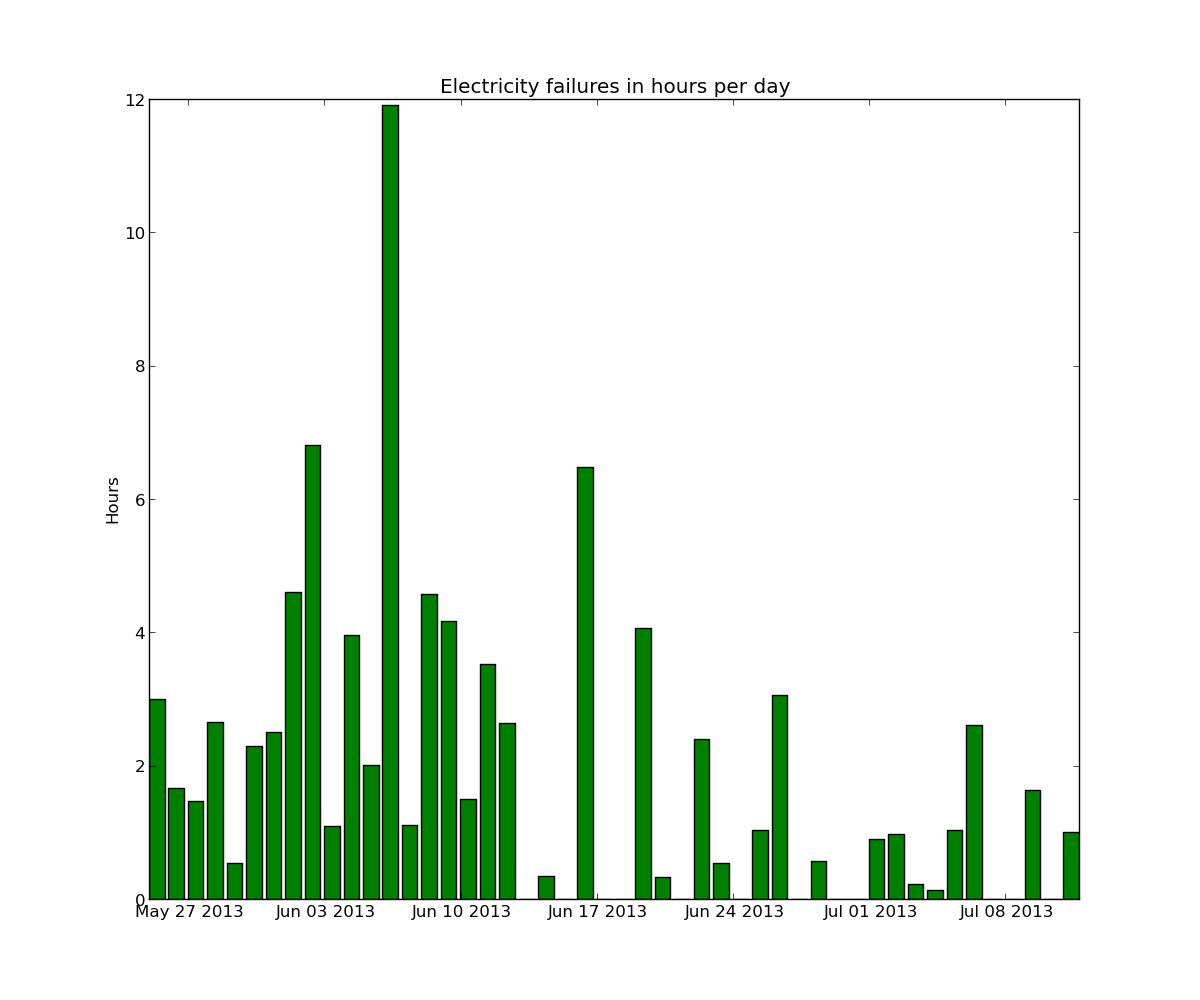
\includegraphics[scale=0.12]{./figures/electricity.png}}
    \hspace{-1mm}    
    \subfloat[\scriptsize Power outage duration ]{
    \label{fig:failure_duration}
    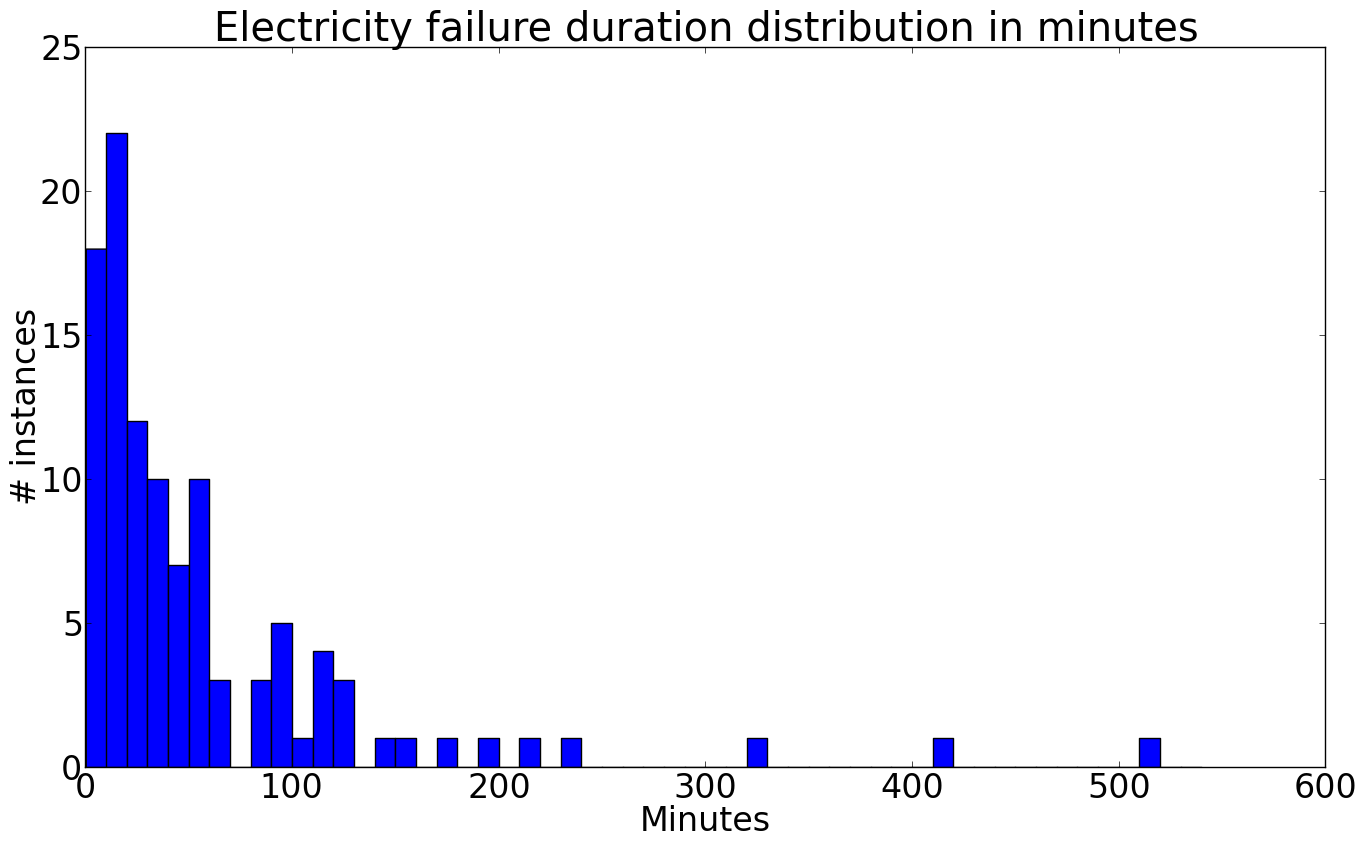
\includegraphics[scale=0.12]{./figures/failure_durations.png}}
    \hspace{-1mm}
    \subfloat[\scriptsize Power outage by hour of day]{
    \label{fig:failure_hour}
    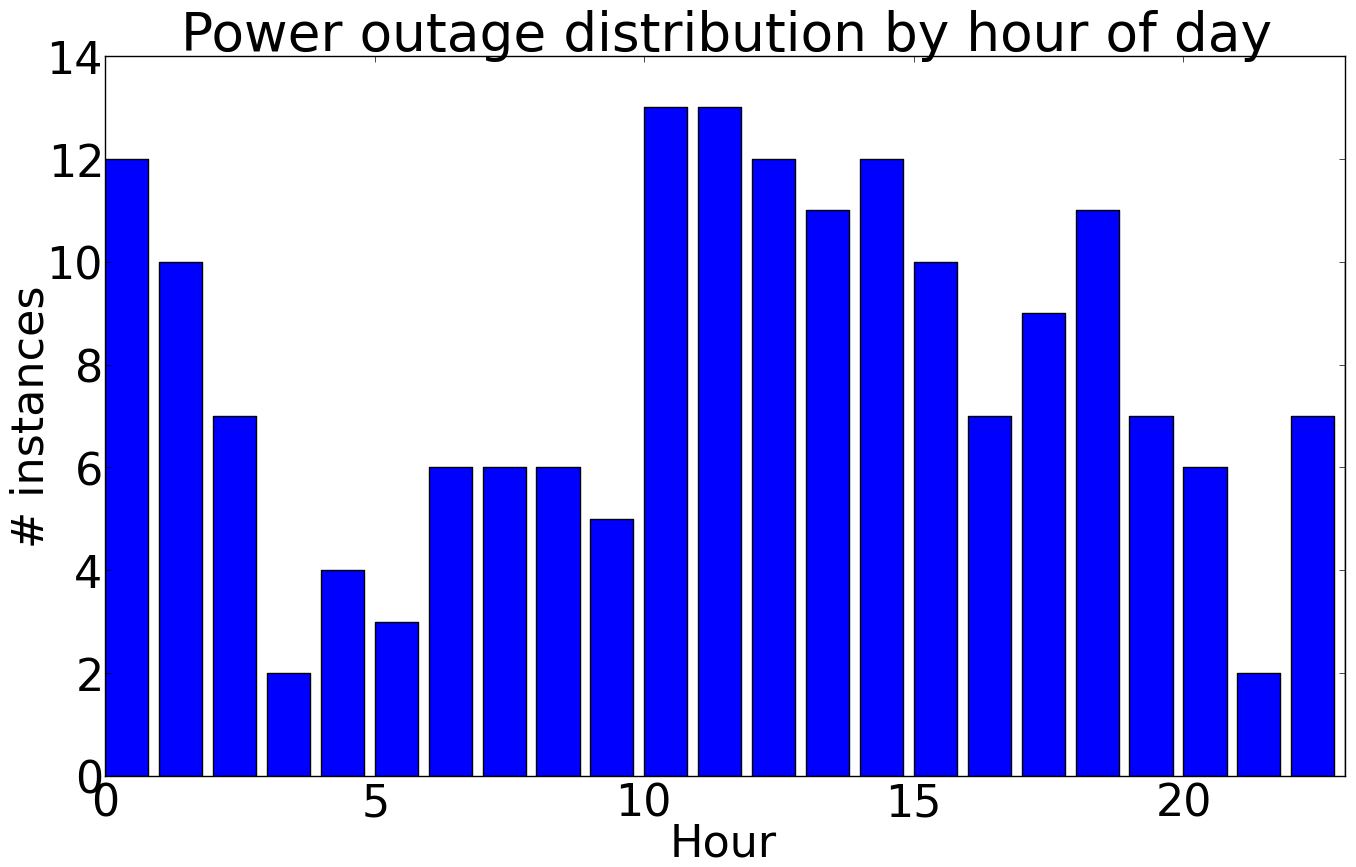
\includegraphics[scale=0.12]{./figures/outage_by_hour.png}}
		\hspace{-1mm}
    \subfloat[\scriptsize Observed voltage just before power outage instances (10 PM to 1 AM)]{
    \label{fig:voltage_before_outage}
    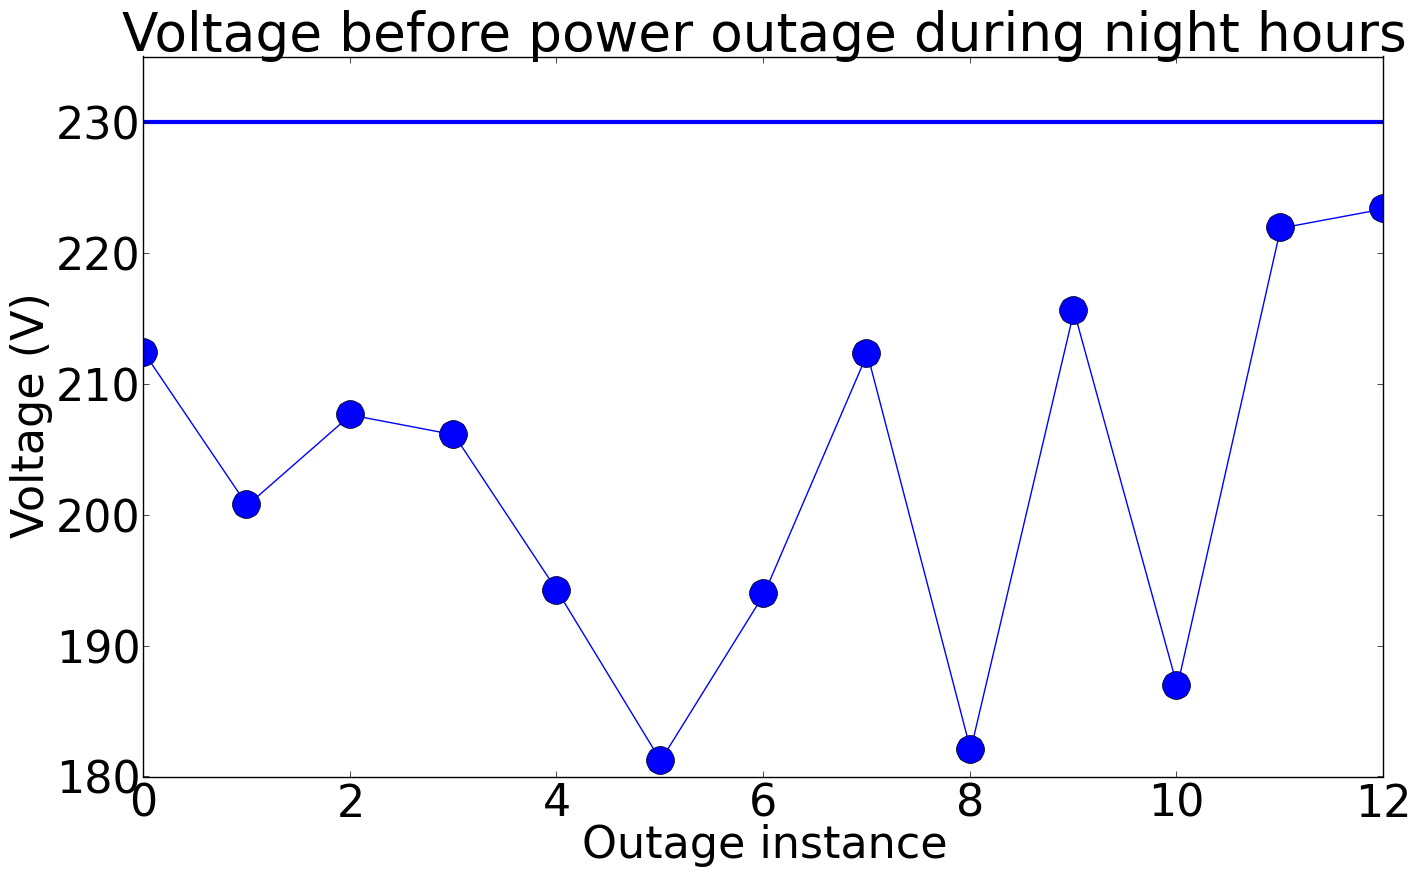
\includegraphics[scale=0.12]{./figures/voltage_before_outage.png}}
		\vspace{-4mm}
		\caption{Illustration of unreliable grid situation during our deployment. Rated voltage in India is 230V.}
    \label{fig:unreliable_grid}
\end{figure*}

		

% % % % % % % % % % % % % % % FIGURE CONTAINING ARCHITECTURE + # Data packets % % % % % % % % % % % % % % % % % % % % % % % % % % % % %
%\begin{figure}
%\vspace{-8mm}
%\subfloat[\scriptsize \paradigm]{
%    \label{fig:architecture}
%    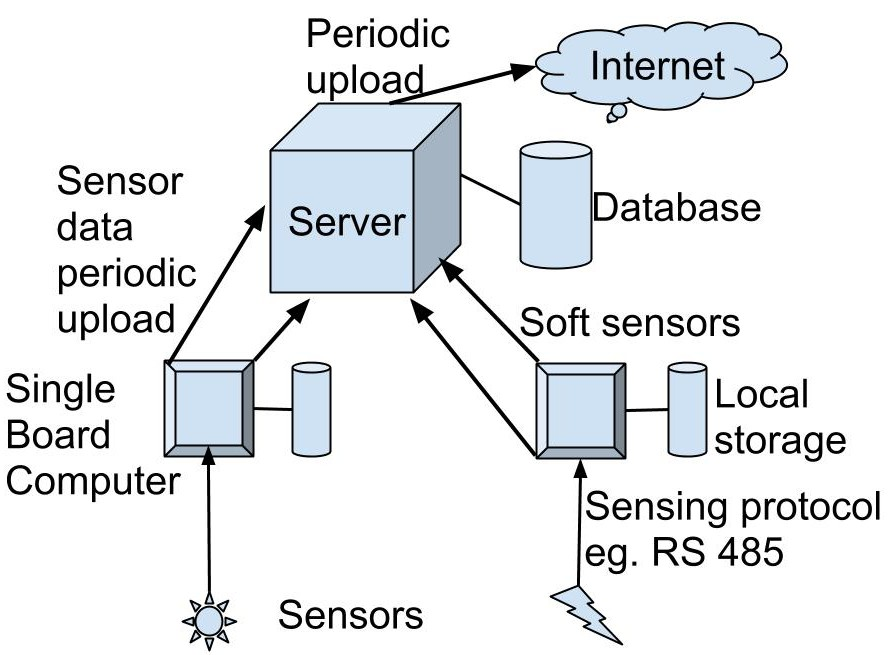
\includegraphics[scale=0.13]{./figures/architecture.jpg}}
%        \subfloat[\scriptsize Amount of data (worth seconds) collected per day from water meter. Data worth 86400 seconds is expected per day. Note that limits on yaxis are raised to ensure that power outage and software losses are visible]{
%        \label{fig:architecture_efficacy}
%        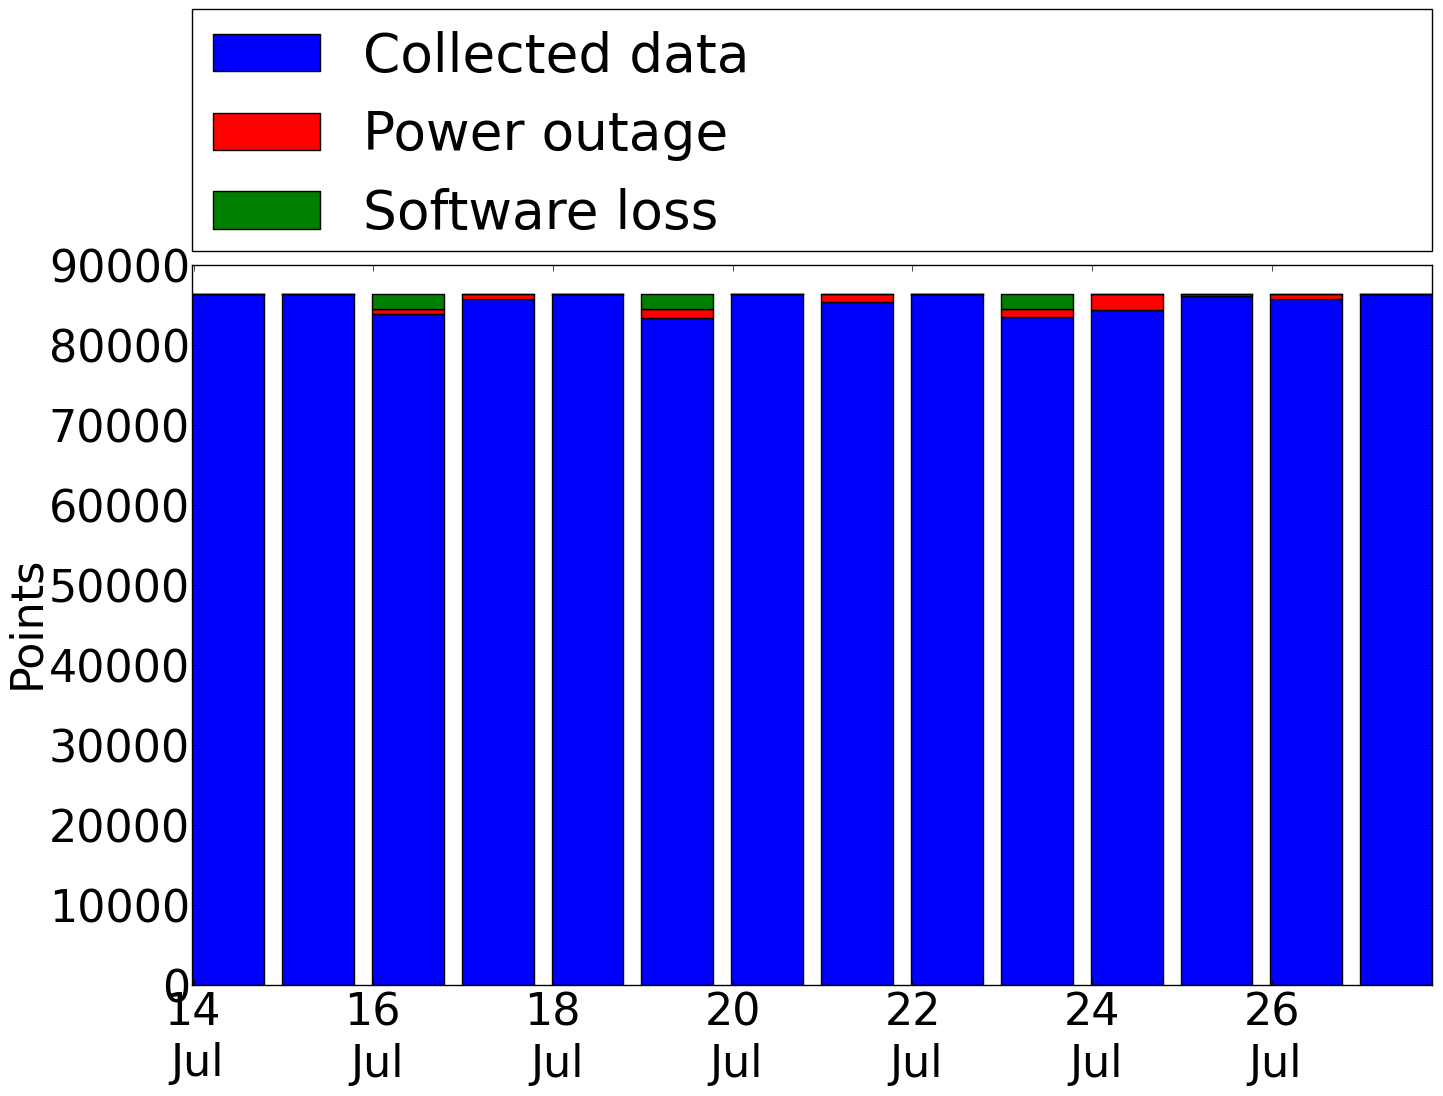
\includegraphics[scale=0.125]{./figures/data_loss.png}}
%        \vspace{-3mm}
%  \caption{\paradigms architecture and its impact on ensuring no data loss}
%  \vspace{-2mm}
%   
%\end{figure}
% % % % % % % % % % % % % % % % % % % % % % % % % % % % % % % % % % % % % % % % % % % % % % % % % % % % % % % % % % % % % % % % % % % %




%\figref{fig:architecture_efficacy} shows the amount of data collected from the water meter during that week.\redcolor{possibly remove the figure, eats up space and does not add much value beyond explanation; moreover can be confusing to the reviewer sparking doubts}


\vspace{-1mm}
\section{How is this deployment different?}
\label{sec:learning}
We now discuss some of the key unique aspects brought forward from our deployment. 

\noindent \textbf{Unreliable electrical grid:} Load shedding or rolling blackout is a commonplace in the developing countries. %owing to several reasons such as improper infrastructure management, high demand and low electricity production. 
Specifically in India, power outages are common in summers when the load is high due to excessive usage of air conditioners. Excessive load and poor infrastructure also leads to significant fluctuations in the supply voltage. %As a result, voltage fluctuations or brownouts are also common.
Various statistics, collected from our deployment, further establish these aspects. We used multiple sources, e.g. Unix \emph{last} command (providing a history of boot times) on the desktop server and common missing data duration from multiple sensors, to find power outages reliably. 

\figref{fig:failure_time} shows power outages in aggregated number of hours per day during May-July 2013. One of the days experienced power outage for approx. 12 hours. 
%(the situation is worse outside of the major cities in India, with electricity coming only for a few hours every day).
 \figref{fig:failure_duration} shows the distribution for duration of all power outages. A total of 107 power outages were reported in the 61 day period reported here, with average power outage of approx. 1 hour. %, there were outages lasting upto 9 hours. 
\figref{fig:failure_hour} shows the power outage distribution by hour of the day, showing maximum outages around 10 AM in the morning and around midnight. These times also correspond to early office time and night time when air conditioners in offices or homes are turned on leading to excessive demand on the grid. \figref{fig:voltage_before_outage} shows that voltage just before the power outage (for a selected sample of outages occurring from 10 PM to 1 AM). We observe that the voltage is well below the rated voltage of 230 V. This is in coherence with previous work~\cite{nplug}, which hypothesized that frequency and voltage measured at the home level are potential indicators of the load on the grid.


\begin{figure*}[t!] 
		\subfloat[\scriptsize Voltage fluctuations in a week (ours)]{
		\label{fig:voltage_box}
    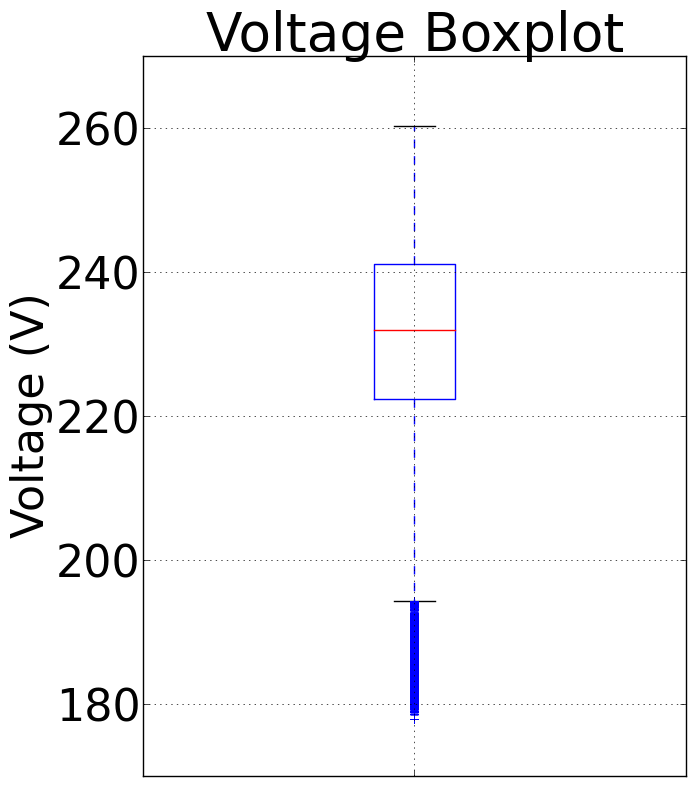
\includegraphics[scale=0.13]{./figures/voltage_box.png}}
    \hspace{1mm}
    \subfloat[\scriptsize Voltage fluctuations in a week (Smart*)]{
    \label{fig:voltage_box_us}
    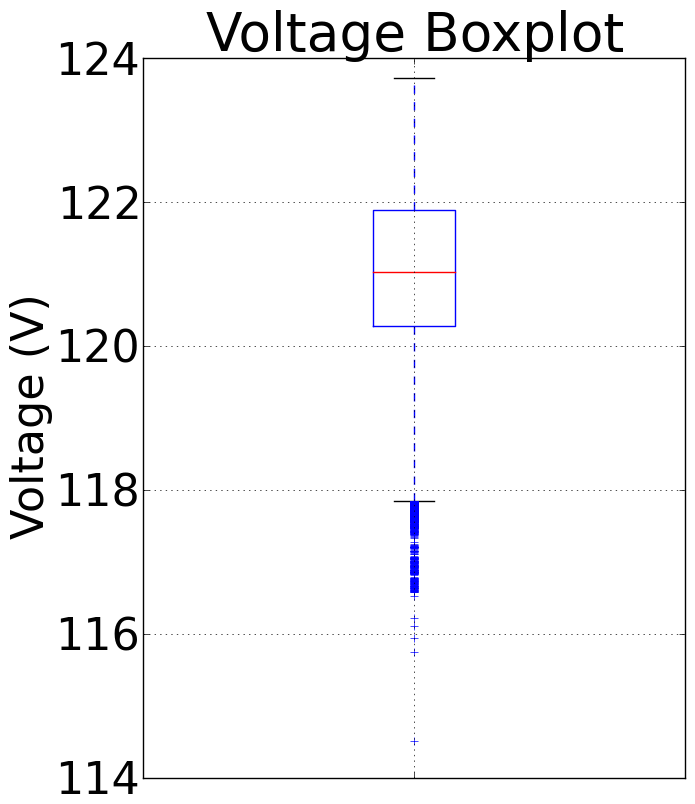
\includegraphics[scale=0.125]{./figures/us_voltage_box.png}}
    \hspace{1mm} 
    \subfloat[\scriptsize Voltage fluctuations on one of the days (ours)]{
    \label{fig:voltage}
    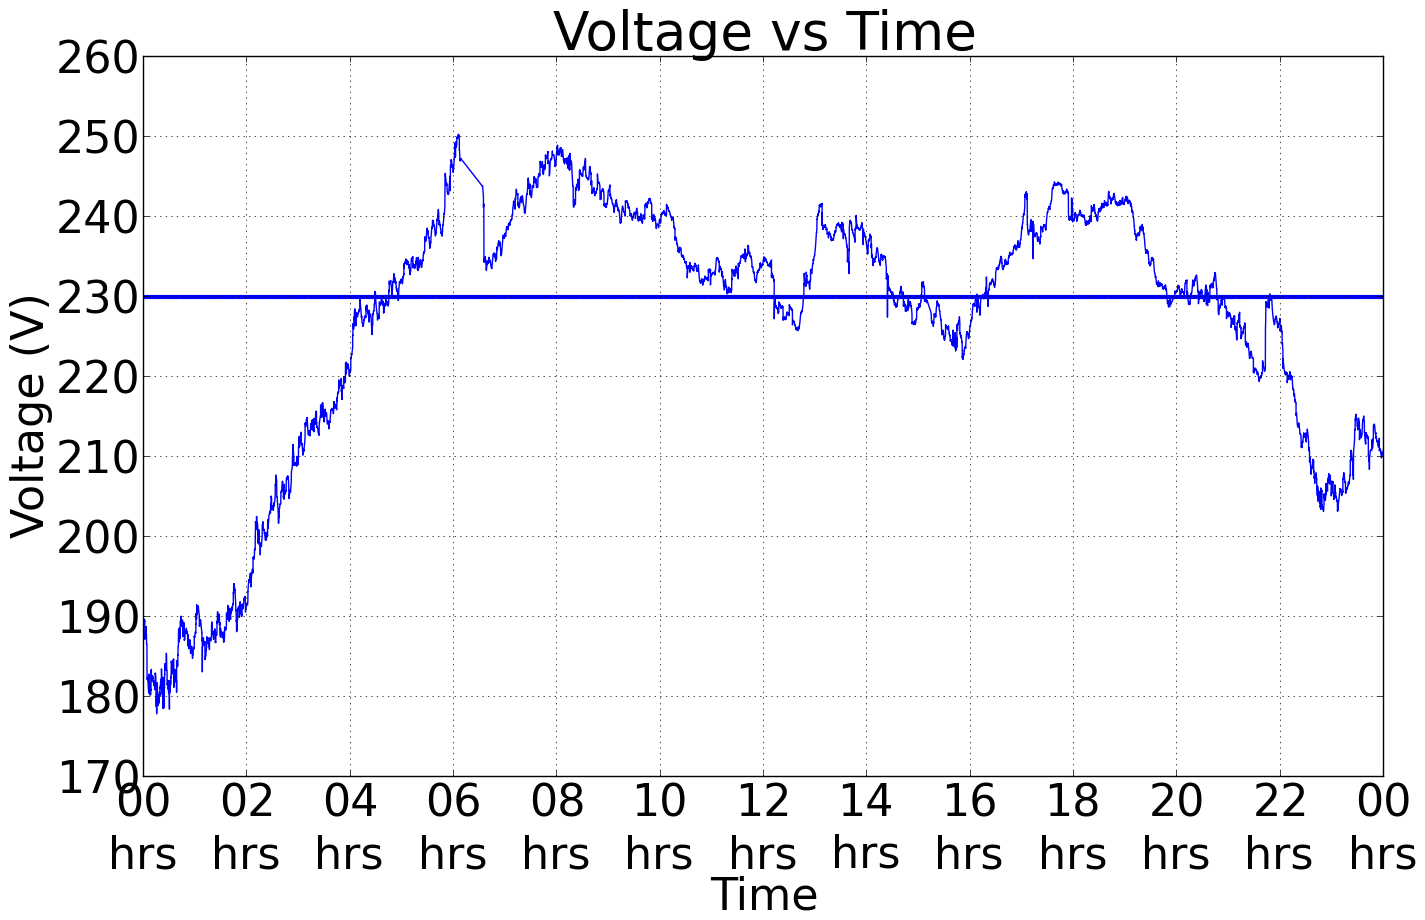
\includegraphics[scale=0.1]{./figures/voltage.png}}
    \hspace{1mm} 
    \subfloat[\scriptsize Voltage fluctuations on one of the days (Smart*)]{
    \label{fig:voltage_us}
    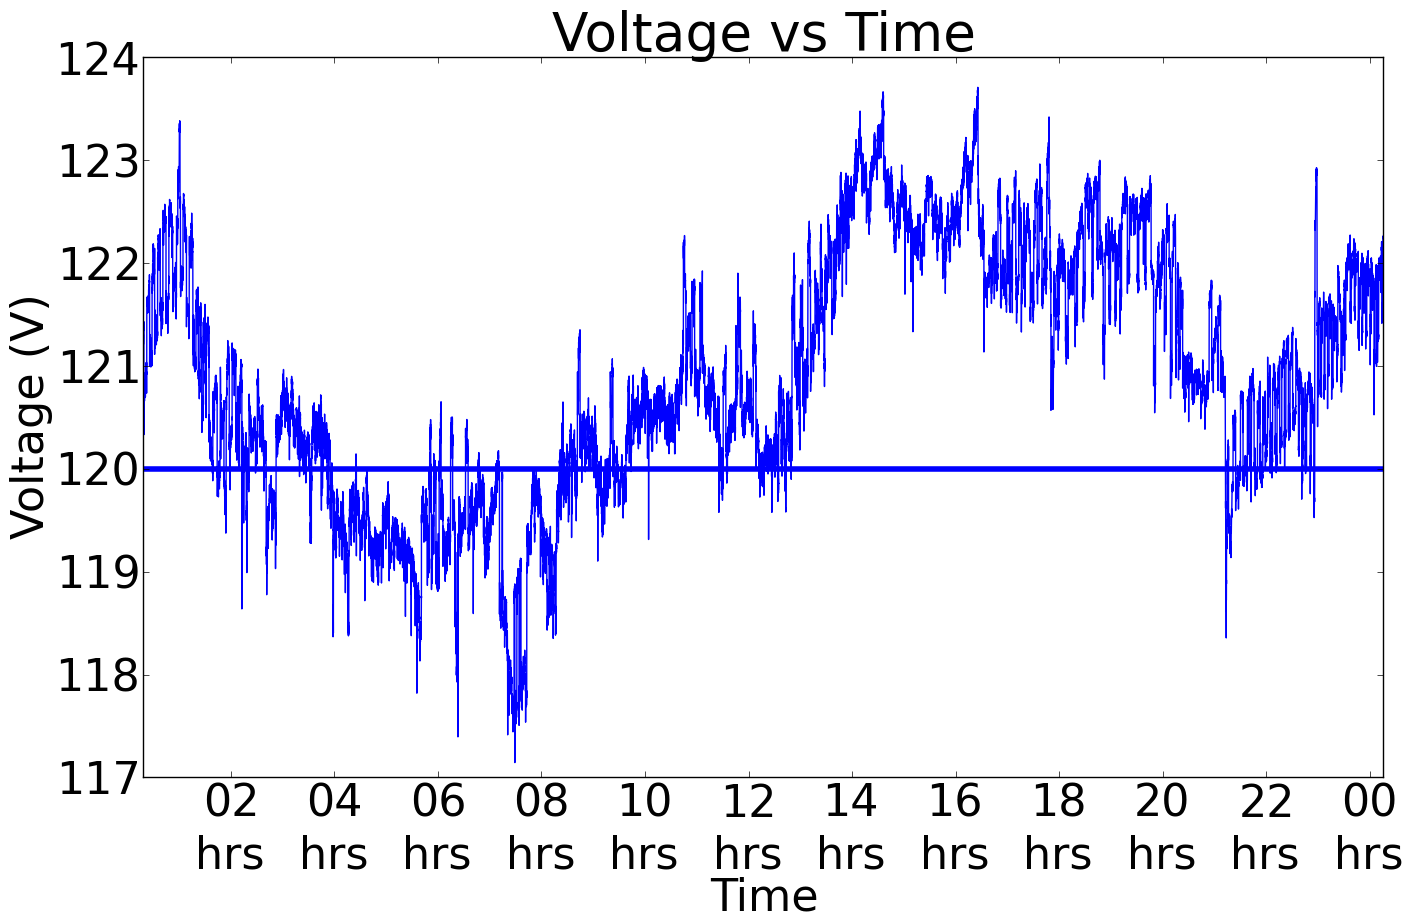
\includegraphics[scale=0.1]{./figures/us_voltage.png}}
    \hspace{1mm}
    \subfloat[\scriptsize Frequency fluctuations in a week (ours)]{
    \label{fig:frequency_box}
    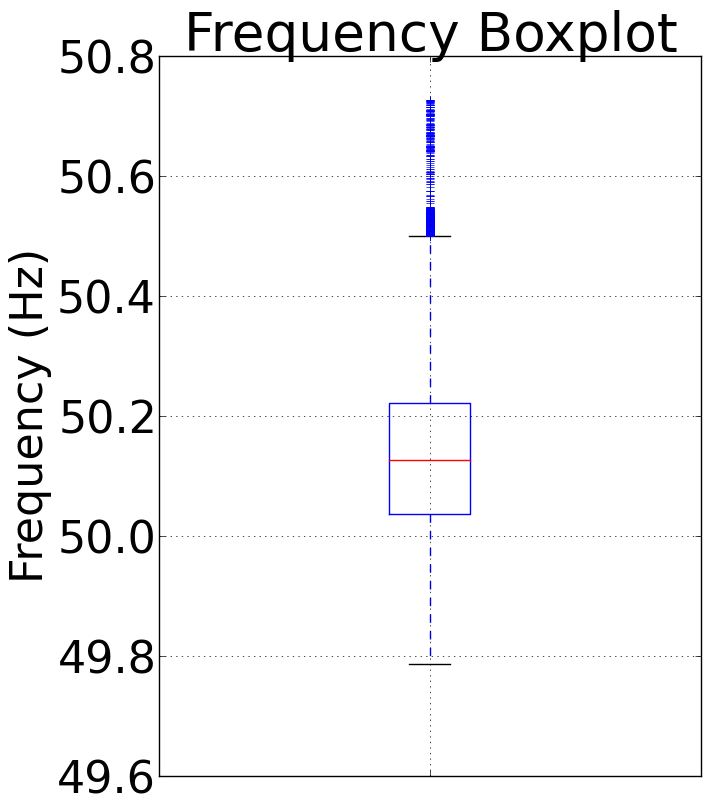
\includegraphics[scale=0.125]{./figures/frequency_box.png}}
    \hspace{1mm}
		\subfloat[\scriptsize Frequency fluctuations in a week (Smart*)]{
		\label{fig:frequency_box_us}
		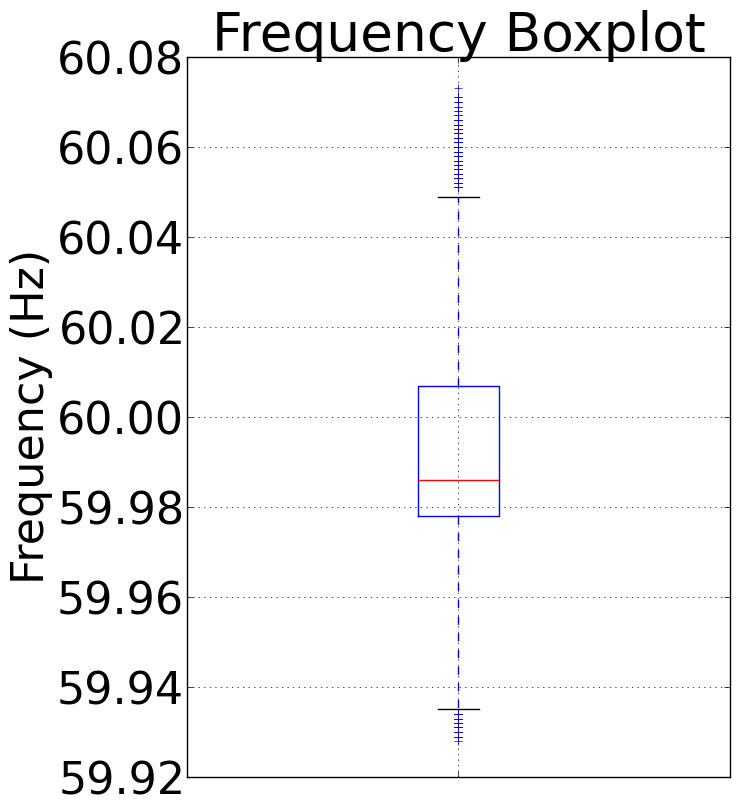
\includegraphics[scale=0.125]{./figures/us_frequency_box.png}}                           
    \vspace{-3mm}
   	\caption{Comparison of our data with Smart* deployment done in the USA}
    \label{fig:unreliable}
\end{figure*}

\figref{fig:voltage_box} and \ref{fig:frequency_box} show voltage and frequency fluctuations for a week in June from our deployment. Comparing these observations with the voltage and frequency fluctuations for a week from Smart* dataset, shown in \figref{fig:voltage_box_us} and \ref{fig:frequency_box_us} respectively, we observe that our deployment shows a lot more variations in both of these parameters. \figref{fig:voltage} and \ref{fig:voltage_us}  show voltage fluctuations on one of the days from our deployment and the Smart* dataset respectively. 
%\figref{fig:voltage} shows the voltage fluctuations, between 180 and 250 Volts, as observed on a typical day. \redcolor{Is it really a typical day? Can you do a box plot for voltage fluctuations for maybe one of the weeks - that will probably have more impact.} 
Significant amount of NILM literature uses current data
%, as measured at different granularity, 
for disaggregation, inherently assuming almost fixed voltage from the grid. 

\textbf{Learning:} \emph{Observed voltage fluctuations motivate two important aspects - 1. Load measurement devices should measure both current and voltage and not only current as is done in many of the CT based devices; and 2. When performing disaggregation, normalization to account for voltage fluctuations (as was proposed in the original NILM work~\cite{hart}) is important.}
%We observe that voltage drops during the peak load hours. 

\noindent Due to unreliable nature of the grid, we wanted to ensure that all our systems were capable of automatically restarting after a power outage and the complete system achieves the same state as it was in before the outage. Correspondingly, data collection and upload scripts were executed as part of system startup process. This feature further provided us with another advantage - when the system was observed to be down, we just asked the home occupant to power cycle the system. This ensured that there was minimal data loss till the time researchers could visit the site and diagnose the fault. %Appropriate logs in the scripts ensured that the fault could be diagnosed in an offline manner.  
With several devices, each with its diverse sensing, computation and communication requirements, ensuring that the system recovers to the same state, as before the outage, was observed to be non-trivial. 

\textbf{Learning:} \emph{A robust building monitoring and control system should be tested for appropriate system recovery after power failure.}


\noindent \textbf{Unreliable network connectivity:} While India has one of the fastest growing internet user base, only 11\% of the total population is connected to internet (the corresponding figure in the USA is 78\%)~\cite{meyer}. %Average connection speed in India is 1.3 Mbps, the corresponding numbers in developed countries are in excess of 10 Mbps~\cite{state_of_internet}. 
%Even though the condition of internet has vastly improved in the previous few years, from practical experience, we have found it to unreliable. 
We observed internet to be either unavailable or having slow intermittent connectivity throughout our deployment. We collected network statistics by performing 15 internet ping requests every 15 seconds and computed the corresponding packet drop. \figref{fig:network} shows that packet drop of up to 22\% was observed on certain days. The average packet drop per day was approx. 6\%. \figref{fig:network_hist} shows a CDF plot of \% packet drop. It can be seen that approx. one-fifths of total days reported greater than 10\% packet loss. %Unreliable internet was the prime motivation behind the proposed \selstups model, discussed in \secref{sec:architecture}. 

\textbf{Learning:} \emph{For a building monitoring and control system to scale up for the context of developing countries, with unreliable internet connectivity, an architecture that does not completely rely on good internet connectivity is important.} %We, thus, believe that for deployments where internet is unreliable, architectures such as \paradigms should be adopted.
%
%\noindent To measure the network connectivity, we collected network statistics by performing 15 internet ping requests every 15 seconds and collected the statistics on packet drop. \figref{fig:network} shows that packet drop of up to 22\% was observed on certain days. The average packet drop per day was approx. 6\%. \figref{fig:network_hist} shows a CDF plot of \% packet drop. It can be seen that approx. one-fifths of total days reported greater than 10\% packet loss. 

We correspondingly propose \paradigms architecture, as discussed in \secref{sec:architecture}, to address for unreliable internet connectivity.

\noindent \textbf{Importance of meta data collection:} We collected metadata associated with electrical appliances, such as appliance name, age, mode of usage (eg. air conditioner set temperature), throughout our deployment. We believe this detailed metadata can enhance NILM and can provide useful insights for conserving electricity. An anecdotal evidence illustrates the utility of meta data collection. The home refrigerator was repaired on 2$^{nd}$ July. \figref{fig:before_repair} and \figref{fig:after_repair} show the active power consumption before and after the repair. We observed that after repair, the refrigerator was set to the lowest temperature setting by the service professional, while before repair it was set to the highest temperature setting. After the repair, the refrigerator was found to be consuming 1KWh more per day (which is 140\% above the normal). The residents configured their refrigerator again to the lowest temperature setting after we informed them about the increased energy usage, resulting in normal power consumption. %returned to previous levels. 
%Moreover, its duty cycle pattern was significantly modified. 
%This metadata can be useful to NILM approaches modeling duration of appliance usage. 
% possible consider % % % % % % % % % % % % % % % % % % % % % % % % % % % % % % % % % % % % % % % % % % % % % % % % % % % % % % %
%
%\redcolor{To make the case even stronger, i am thinking of putting the need for measurement calibration for different h/w}
% % % % % % % % % % % % % % % % % % % % % % % % % % % % % % % % % % % % % % % % % % % % % % % % % % % % % % % % % % % % % % % % %
%\redcolor{Was this increased energy with higher setting or even after you reduced the setting?}

\noindent \textbf{Load specifics:} Appliance usage varies significantly in India compared to the USA and the Europe. 

\emph{Decentralized control:} Temperature control is often decentralized in the Indian settings i.e. a separate air conditioner is used for every room and a separate geyser (a water heating device) is used for each bathroom. From our deployments, we observed that these air conditioners and geysers account for up to 70\% and 50\% of the overall home electricity in summers and winters respectively. Thus, small improvements in efficiency of these two appliance can significantly lower the home electricity consumption. From NILM perspective, these loads are simpler to disaggregate due to their high power consumption and repeated patterns (shown by the compressor in the air conditioner). 

\textbf{Learning:} \emph{Even a simple NILM approach can potentially provide useful insights towards energy reduction in the Indian context.}

We are currently working on testing different NILM approaches, e.g. Combinatorial optimization and Hidden Markov Models, on our collected data.

\emph{Energy embedded water:} Additional energy, in the Indian context, is embedded into the water at the home level due to its low pressure and poor quality. Water pumping and filtering are the two activities whose scope spans across both water and electricity dimensions. Due to limited supply and line pressure, a water motor is used to pump the water up to the water tank on the roof. We observed that to fill 1 liter of water into the tank, it took 8 seconds without the motor (during the times of maximum pressure) and 4 seconds when the motor was used. With power consumption of 700 W for the electric motor, every one hour usage will result in additional energy being embedded into the water due to its intermittent supply. % was approx. 700 W. To fill an empty water tank (\redcolor{mention its capacity}) it would take 8000 seconds (2 hours 12 mins) without motor and 4000 seconds (1 hours 6 mins) with motor. An additional 770 Wh energy would be consumed if the motor is used. Thus, there is a fine balance between electricity consumption and time taken to fill the tank. We found that motor is typically used for 10 minutes in a day.
%Since water flow from utilities is provided only for about 1 hour each in the morning and evening, motor is used for about 10 minutes a day.
Due to poor quality of supplied water (and often usage of ground water for drinking purposes), Reverse Osmosis based water filters are a commonplace in big cities in India. We observed that water filter takes approx. 1 minute to filter 1 liter of water and consumes 40 W in the process. 
%Thus, the water filter would consume 20 Wh energy for filtering 30 liters of water (typical drinking water usage).

\textbf{Learning:} \emph{Observing water consumption, together with the electricity consumption, can provide additional useful insights in usage and consumption patterns.}
\begin{figure} [t!]
\vspace{-4mm}
\subfloat[\scriptsize \% internet packet drop vs time]{
    \label{fig:network}
    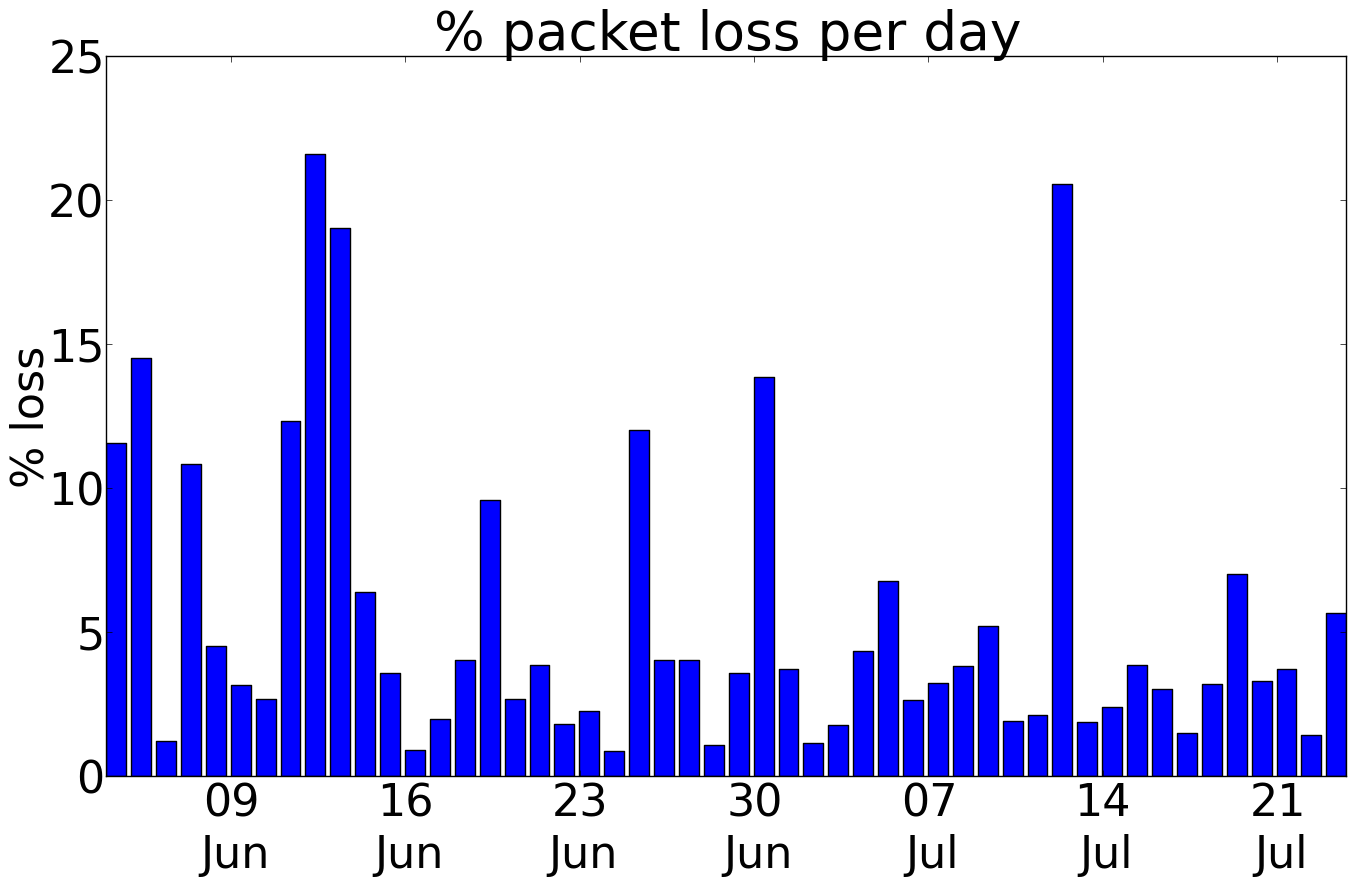
\includegraphics[scale=0.11]{./figures/network.png}}
        \subfloat[\scriptsize \% internet packet drop CDF]{
        \label{fig:network_hist}
        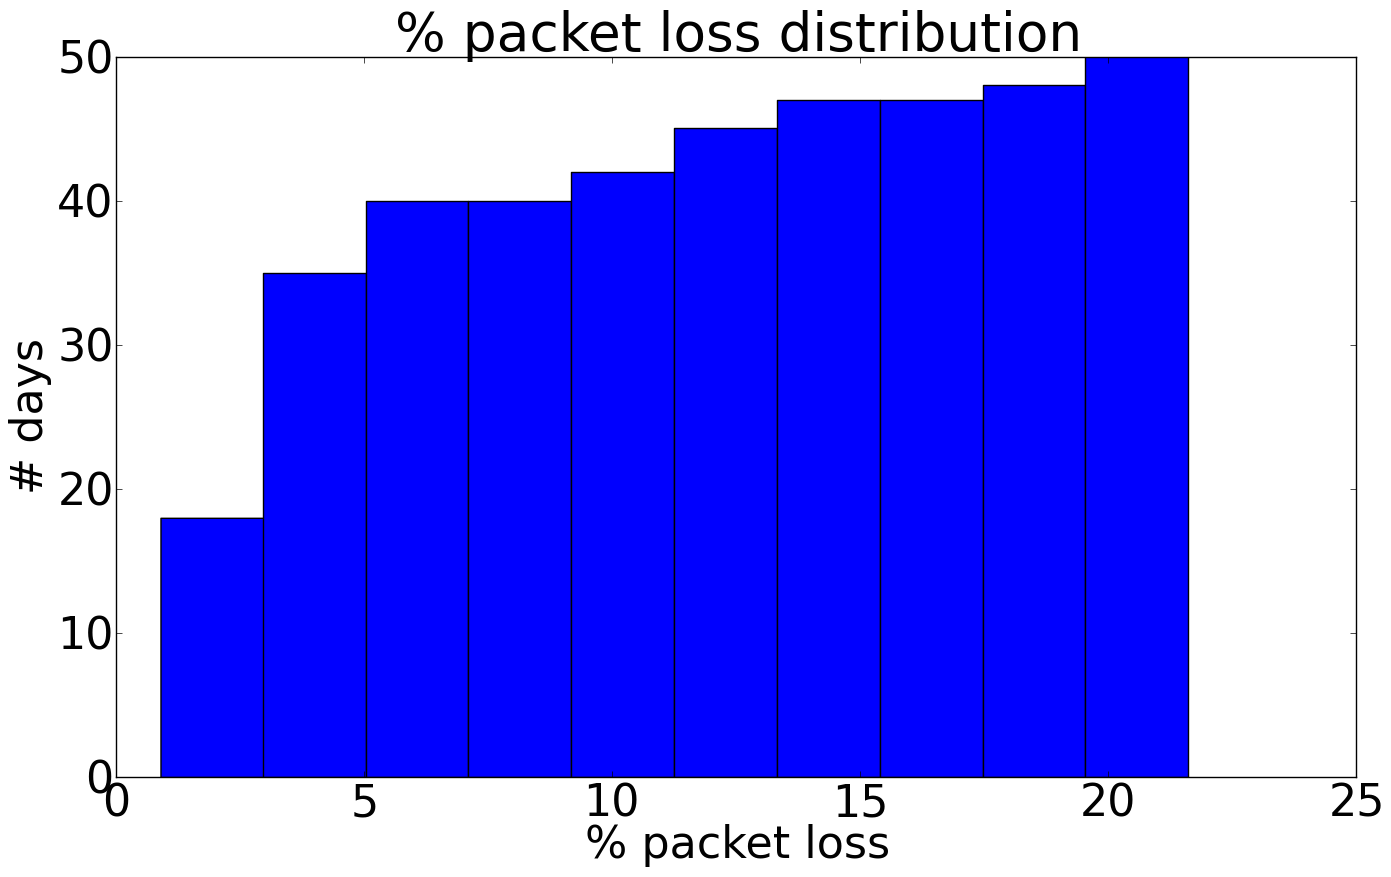
\includegraphics[scale=0.11]{./figures/network_hist.png}}
        \vspace{-3mm}
  \caption{Unreliable internet}
  \vspace{-2mm}
  
      \label{fig:unreliable_internet}
\end{figure}

\begin{figure}[t!]
\vspace{-2mm}
\subfloat[\scriptsize Before repair]{
    \label{fig:before_repair}
    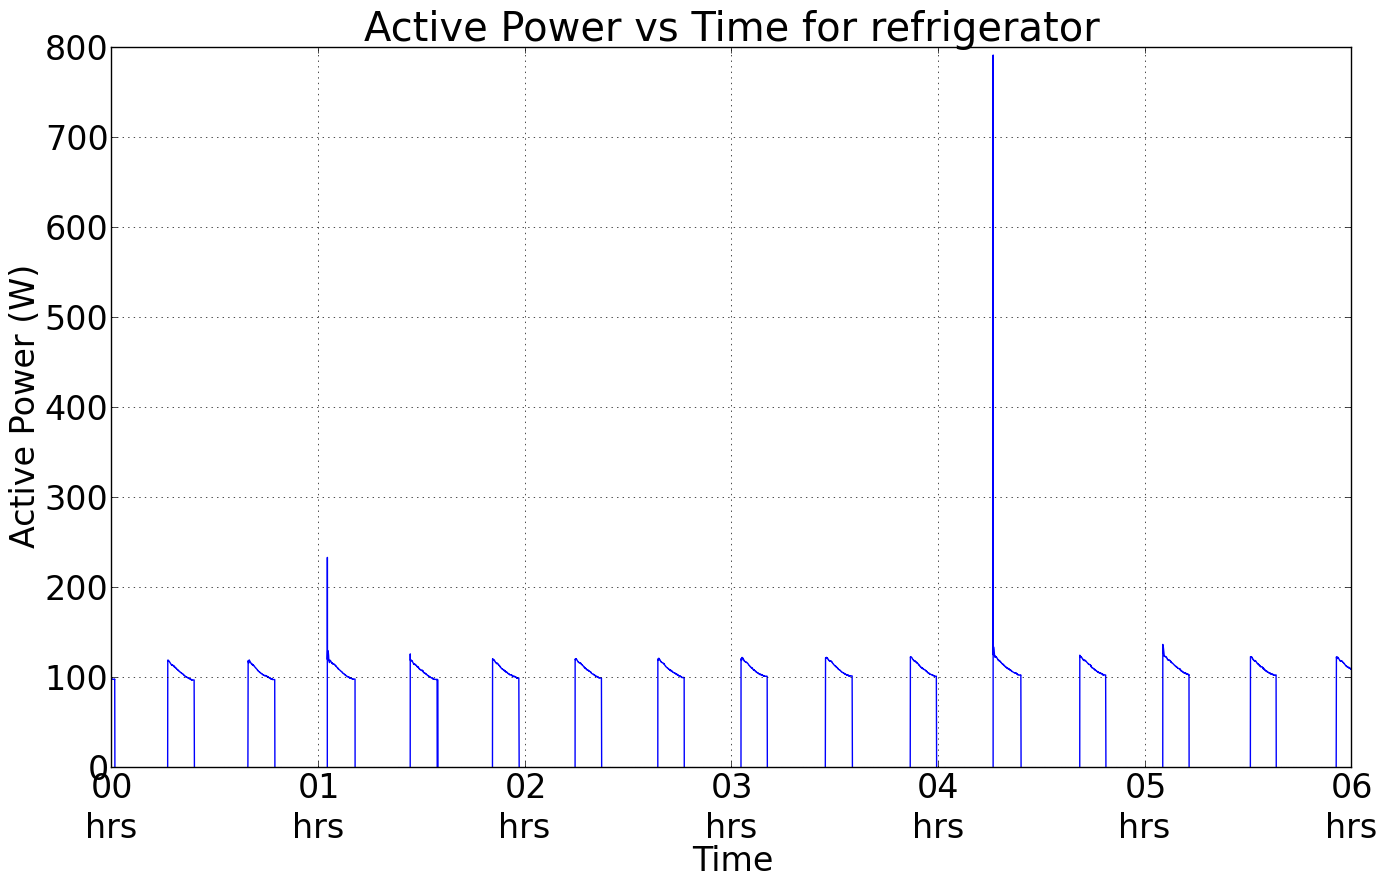
\includegraphics[scale=0.1]{./figures/before_repair.png}}
     \subfloat[\scriptsize After repair ]{
        \label{fig:after_repair}
        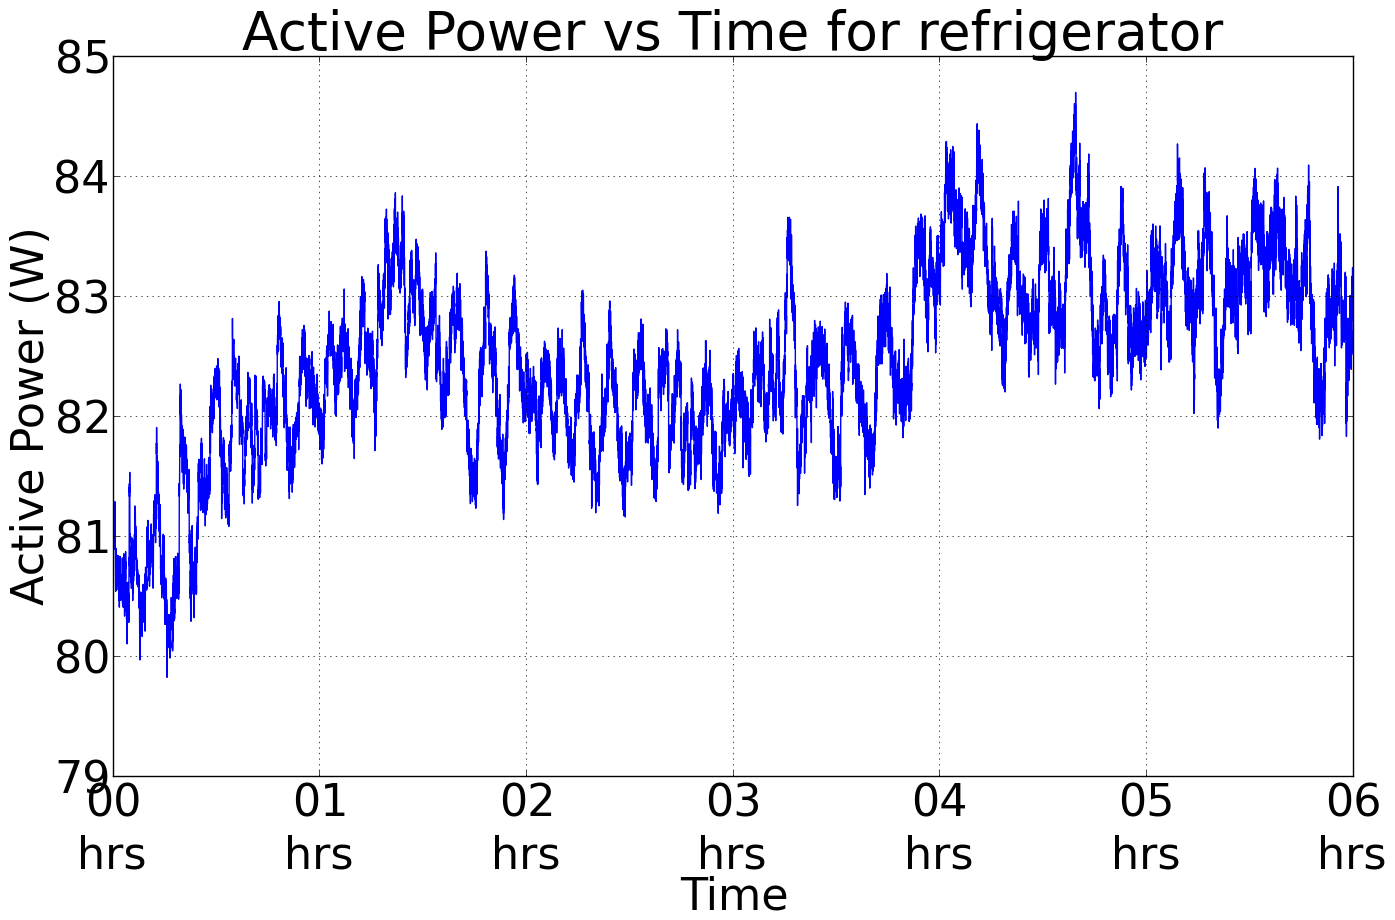
\includegraphics[scale=0.1]{./figures/after_repair.png}}
       
   \vspace{-3mm}
    \caption{Refrigerator power consumption}
    \label{fig:metadata}
    \vspace{-4mm}

\end{figure}
	

\emph{Appliance switching from mains:} Another interesting distinction in the Indian context is that each plug point has an associated switch and people are often conscious about turning the appliance off from the switch rather than keeping them in the standby (as is the usual practice in the USA). We observed that the jPlugs attached to the kitchen appliances such as microwave, when used for less than 1 minute, did not report data. This was due to the fact that jPlug setup takes roughly a minute to establish WiFi connectivity before starting the data collection. For small usage, before jPlug could start data collection, the appliance was turned off.

We also imported ZWave based plug monitors and controllers (with EU frequency) for plug level monitoring. After their initial deployment, we realized that the default state of the plug monitors was chosen as off (when powered manually from the switch), possibly to avoid the peak switching current. This implied that even after switching them on from the mains, unless they are switched on from the software (or with a separate ZWave based switch), they will not turn on the appliance. Since many of the loads in the Indian context are not always on and are controlled via mains, such plug sockets did not result in seamless usage. 

\textbf{Learning:} \emph{Plug level monitoring should account for the short appliance usage and power off from the main switch to ensure robust and reliable data collection, together with seamless usage.}

%If the appliances were to be always on, this data would not have been lost. 
%From our survey with the home occupants, we found that their 
% We seek to resolve this issue in our future deployments.


\begin{figure}

\centering 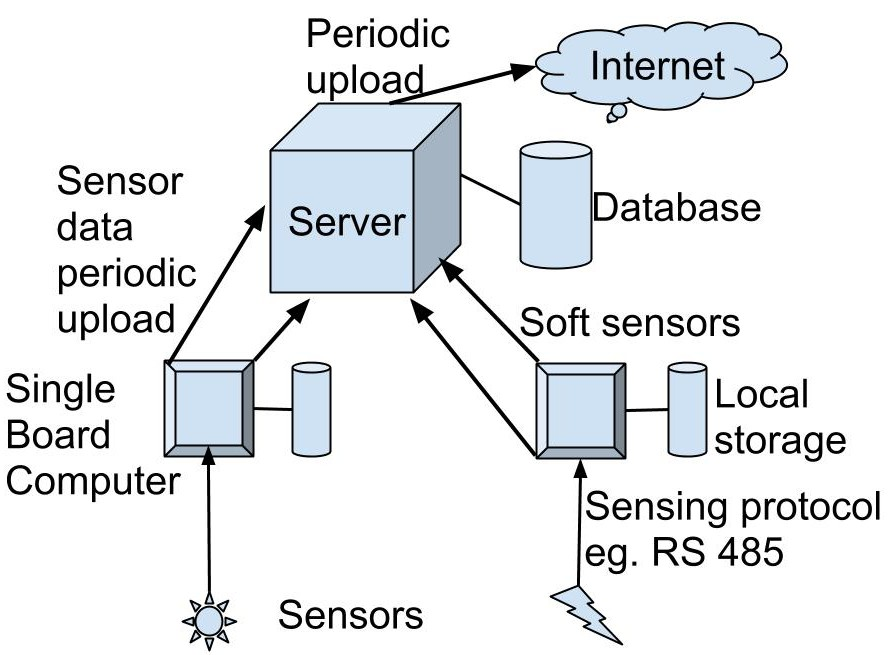
\includegraphics[scale=0.12]{./figures/architecture.jpg}
\vspace{-2mm}
\caption{\paradigms architecture}
\vspace{-2mm}
\label{fig:architecture}
\end{figure}

\vspace{-1mm}
\section{\paradigms Architecture}	
\label{sec:architecture}
Middleware systems such as sMAP~\cite{smap}, BuildingDepot~\cite{buildingdepot} and SensorAct~\cite{Arjunan12} have been proposed in the past for sensor data collection from deployments pertaining to buildings. However, we found that they do not sufficiently address the requirements of our deployment context e.g. intermitted network connectivity and repeated power failures. Motivated by our experience as well as previous work from other researchers~\cite{hitchhiker_residential}, where importance of simplifying the architecture are proposed, we propose \paradigms (\selstup) model. \selstups involves two main ideas - association of local storage (using SBCs) distributed across each sensing point and periodic data upload (from SBC to server, and from server to cloud). As discussed in \secref{sec:comm_comp}, we used 6 SBCs (and local storage on the Android phones) to connect to multiple sensors spread through our deployment. Data collected from the sensors was \textbf{locally stored} in the form of comma separated value files (CSV), in SBCs and \textbf{periodically uploaded} to the main desktop server. In the case when upload failed, it was retried after a fixed time duration. Each SBC was provisioned with sufficient flash based local storage to accommodate sensor data for a few days, to account for persistent upload failure.

Web applications running on the server allowed residents to locally visualize their data from multiple sensing streams. Data from the server was periodically replicated to the cloud, allowing researchers to remotely visualize the data and maintain the deployment. \figref{fig:architecture} illustrates the \selstups architecture. The salient features of \selstups architecture are:


\noindent \textbf{Decoupled sensing and data upload:} ensuring that an error in data upload does not impact the sensing and vice versa, thus avoiding data loss due to network (even the local in-home WiFi) failure. %The design choice of decoupling comes from the well established principles of software engineering.

\noindent \textbf{Reduced dependence on always-on connectivity:} Internet is required \textbf{only} when outside researchers wish to view data in near-realtime. Internet failure does not have any impact on the deployment data collection. The periodic nature of our uploads ensured that data would be uploaded when internet connectivity is re-established. Local storage, on SBC, further ensures reliable data collection, even in the cases of server failure. %Further, there is no data loss even if the server goes down for some time, due to local storage.

\noindent \textbf{Reduced load on server:} Periodic upload of data (in larger volumes) results in reduced computation and bandwidth requirements for the SBCs and the server. 
%While it comes at the cost of increased storage requirements on SBCs, our analysis shows that 1 GB of local storage will suffice for most of the practical scenarios. %, we did not need to provision for more than 1 GB.

We provide anecdotal evidence to illustrate utility of \selstups in preventing data loss. One of the researchers involved, accidentally killed the server script responsible for collecting water consumption data. However, when the problem was rectified a week later, all the data for the previous week, which had been locally stored on the RPi, was collected within an hour on the server. 


\vspace{-1mm}
\section{Hitchhiker's guide revisited}
\label{sec:common}
We now present some of the prominent similarities, albeit with some additional unique perspectives, with prior deployment experiences, most specifically - ``The Hitchhiker's Guide to Successful Residential Sensing Deployments"~\cite{hitchhiker_residential}. 

\noindent \textbf{Homes are hazardous environments:} We observed that one of our multisensors repeatedly failed after every power outage. %Initially, we felt that the sensor was faulty, but other multisensors also showed the same behavior in the same location. 
We, eventually, figured that this behavior was due to the fact that this multisensor was put on the battery backup plug (commonly available in many homes to guard against intermittent power supply) and would not fail during the power outage. When the main power resumed, ZWave controller was not able to add this multisensor to its network, as the multisensor had gone to \emph{sleep} in its absence and was assumed to be \emph{dead}. We resolved this by putting the multisensor on the main plug as well. %We also observed that one of the multisensor would always indicate motion. Initially we solved this problem by replacing its power supply. However, within a week, this problem resurfaced. We believe it is due to the faulty power supply in that room. The home occupants did not allow a thorough investigation of that electrical socket and we had to do away with that data.
Although we used zip-ties extensively throughout the deployment to prevent hanging wires, we observed data loss in one of the ZWave multisensor and an Android phone, which went out of power due to wire snag (shown in \figref{fig:snag}). Even after a month of rigorous testing in the lab before we started the deployment, we raised 60 new service complaints, when we moved the deployment to the home. %This is a testimony that homes present unique challenges which can not be exactly emulated in laboratory settings.

\noindent \textbf{Aesthetics matter:} As stated in the previous work, sensor LEDs can be bothersome to the occupants, particularly in the night. Our deployment introduced 63 LEDs in the home. \figref{fig:led} shows our sensor LEDs blinking in the night. Choosing appropriate sensor location sufficed for the current deployment. However, for the future, we intend to case the sensors appropriately to ensure that home occupants are not disturbed. The residents also complained of buzz like sound coming from our desktop server. This noise was due to the dust clogging in the desktop. Dust is a uniquely common aspect in the Indian setting. 

\textbf{Learning:} \emph{Monitoring and control systems, aiming for long life deployments should include routine maintenance, to guard against dust and other environmental problems.}

\noindent \textbf{Homes are not designed for sensing:} We observed much more noise in the data collected from our ground floor MCBs than from the MCBs on the first floor. This was attributed to the fact that the MCBs on the ground floor were close (as shown in \figref{fig:ct_interference}) to each other causing interference in our CT monitoring circuit. A workaround could have been to get additional cabling done, but the residents were not inclined for such changes. %For the 3 MCBs on the first floor, there was adequate gap amongst them and the data was of good quality (verified using manual experiments involving switching appliances on those circuits). %We, thus, believe that homes are not designed for sensing and one may not be able to sense desired parameters.

\noindent \textbf{Redundancy-Accounting for sensor failure:} During our deployment 3 jPlugs and 1 multisensor stopped functioning. We had accounted for such failure and had kept reserve sensors ready. %We believe that one should beforehand account for sensor failure in residential deployments.

\noindent \textbf{Homes have poor connectivity:} During the preliminary phase of our deployment, we first tried to connect our sensors to the existing networking infrastructure in the home. Already existing WiFi router was on the first floor and we observed poor signal strength on the ground and the second floor. We used Ekahau Heat Mapper\footnote{\url{www.ekahau.com/products/heatmapper/overview.html}} to map WiFi signal strength. \figref{fig:ground_without_router} and \ref{fig:second_without_router} show the WiFi heatmap produced with the home router placed on the first floor. We observed that large regions inside the home show poor signal strength. We bridged additional routers on the ground and the second floor with the existing first floor router. \figref{fig:ground_with_router} and \ref{fig:second_with_router} show the corresponding WiFi heatmaps produced after the introduction of bridged routers. Additional routers significantly improved WiFi coverage across the home, shown by increased green regions (signifying better signal strength as per the scale shown in \figref{fig:heatmap}). 

%\noindent Another important facet of deployments is that additional sensors introduced inside a home may choke up the network bandwidth. We observed this when we tried using imported WiFi based microcontrollers for sensing ambient conditions in our research wing. Research wing occupants complained of low network bandwidth available for their personal usage. Thus, we decided to use ZWave based multisensors for measuring ambient parameters for home deployment. Since ZWave based sensors worked on a different frequency (868.4 MHz) as WiFi(2.4 GHz), they did not cause interference. We believe that a careful mix of sensors working on different frequencies can be used to avoid interference issues.

% % % % % % % % % % % % % % % % % % % % TABLE % % % % % % % % % % % % % % % % % % % % % % % % % % % % % % % %
%\begin{table}
%\tabcolsep=0.015cm
%\vspace{-4mm}
%\caption{First floor water fixtures labeled metadata}
%\vspace{-4mm}
%\label{tab:water_consumption_labeled}
%\footnotesize
%\begin{tabular}{|c|c|c|c|c|}
%\hline
%\textbf{Sno.}&\textbf{Type}&\textbf{Consumption}&\textbf{Purpose}&\textbf{Location}\\
%\hline
%1&Flush&10 liters per flush; 210&Toilet&Bathroom\\
% &&seconds for flush tank to refill&flushing&cum toilet\\ \hline
%2&Tap&17.5 l/minute&Washing clothes&Washing area\\ \hline
%3&Tap&5 l/minute&Washing hands&Washbasin\\ \hline
%4&Tap&7 l/minute&Bathing&Bathroom\\ \hline
%5&Tap&1 l/minute&Bathroom cleaning&Bathroom\\ \hline
%6&Tap&13.2 l/minute&Gardening&Veranda\\ \hline
%
%\end{tabular}
%%\vspace{-6mm}
%\end{table}
\begin{figure}[t!]  
%\vspace{-2mm}
\subfloat[\scriptsize Ground floor (without additional router)]{
	 \label{fig:ground_without_router}
    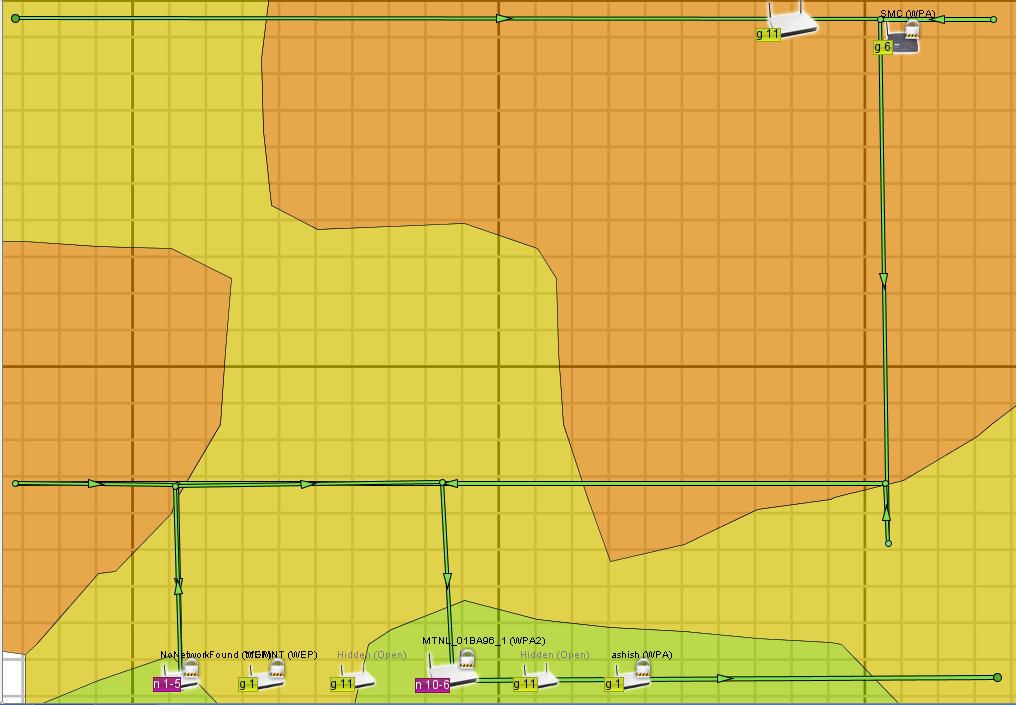
\includegraphics[scale=0.05]{./figures/ground_without_router.png}}
    \hspace{0.4mm}
    \subfloat[\scriptsize Ground floor (with additional router)]{
    	 \label{fig:ground_with_router}
        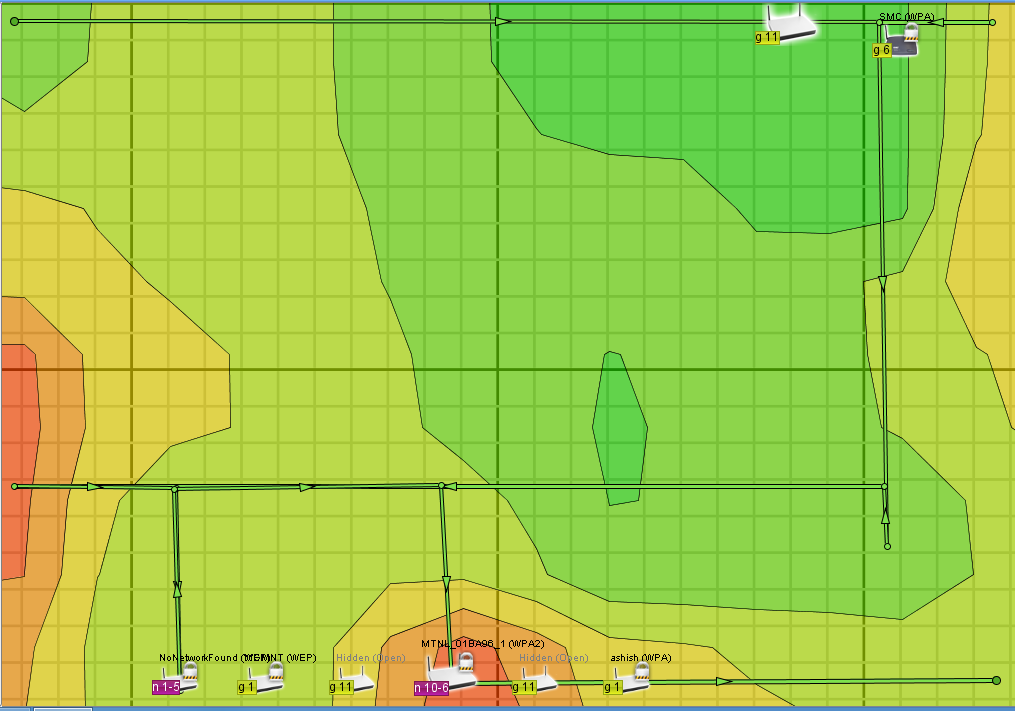
\includegraphics[scale=0.05]{./figures/ground_with_router.png}}
%       \subfloat[]{
%       	 \label{fig:heatmap}
%           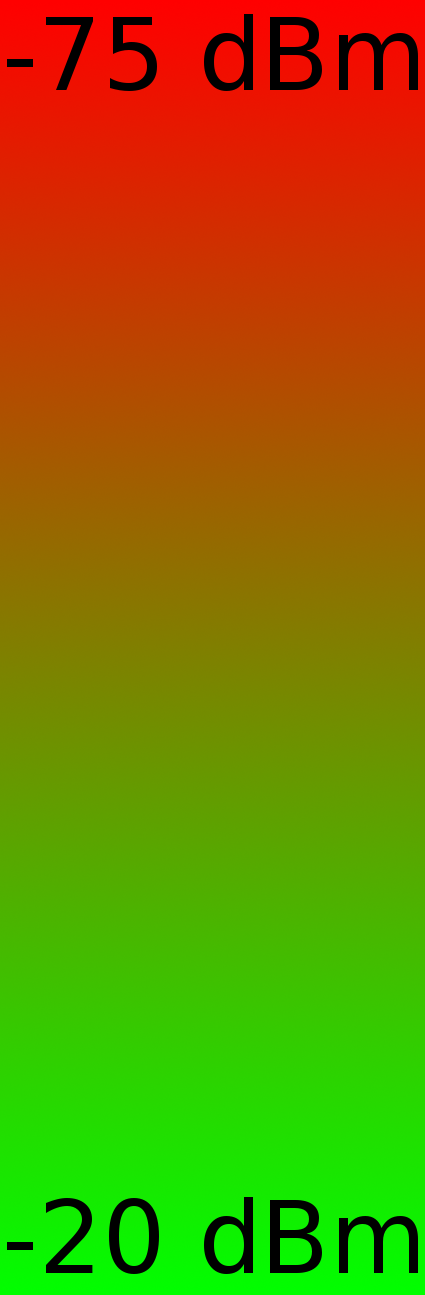
\includegraphics[scale=0.1]{./figures/heatmap.png}}
%        \vspace{-3.5mm}
%       \newline
\hspace{0.4mm}
      \subfloat[\scriptsize Second floor (without additional router)]{
      	 \label{fig:second_without_router}
          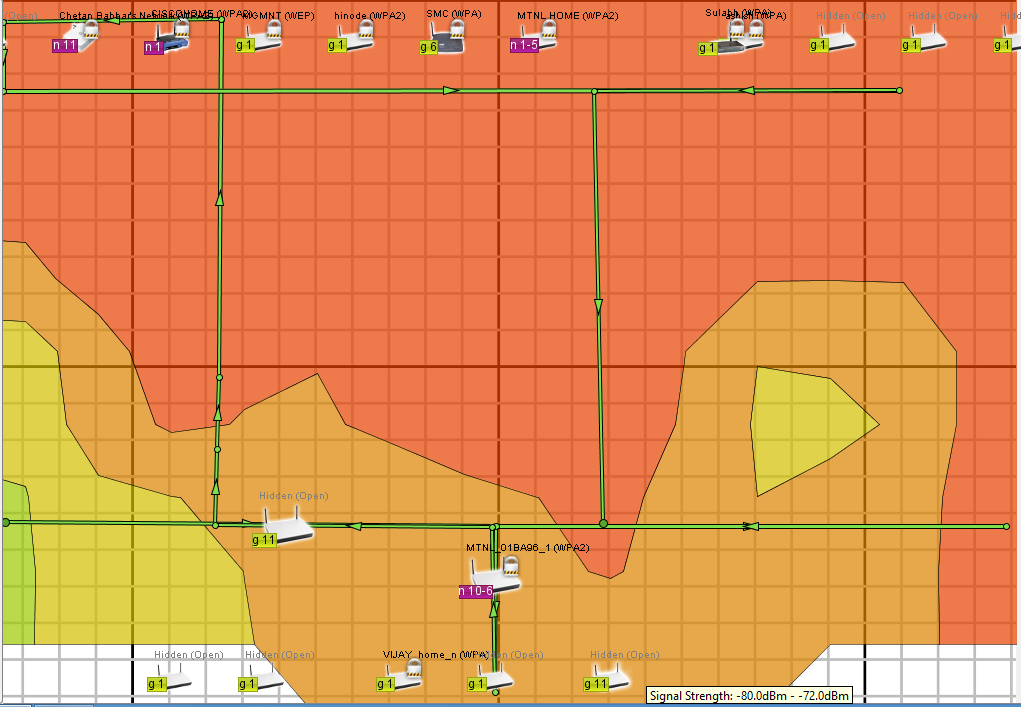
\includegraphics[scale=0.05]{./figures/without_.png}}
          \hspace{0.4mm}
          \subfloat[\scriptsize Second floor (with additional router)]{
          	 \label{fig:second_with_router}
              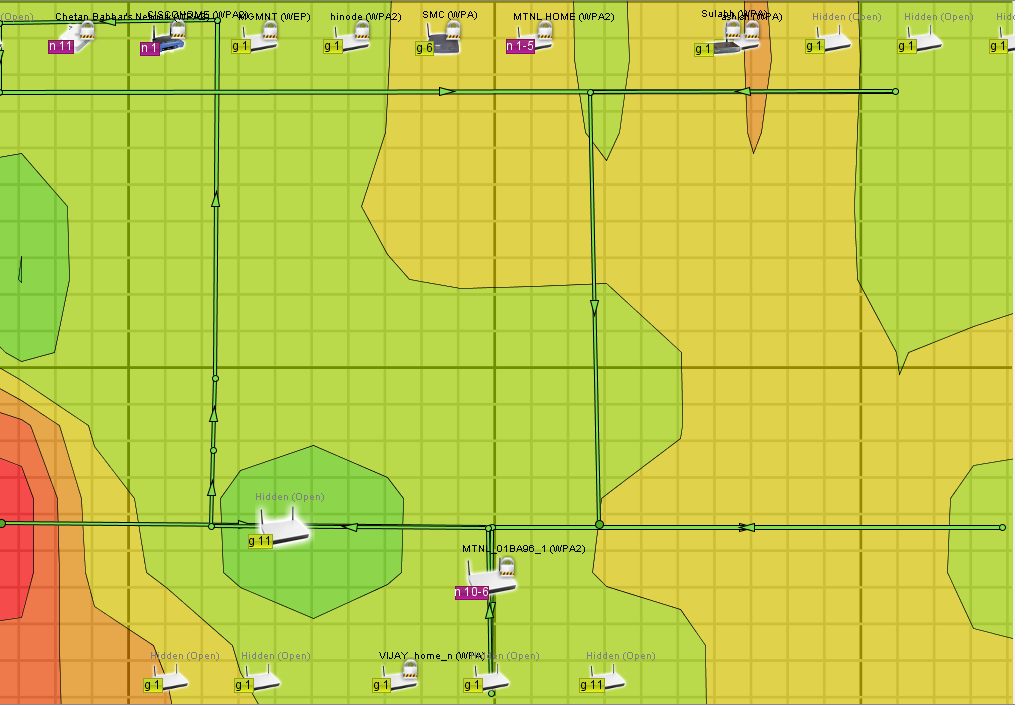
\includegraphics[scale=0.05]{./figures/with_.png}} 
              \hspace{0.4mm}
              \subfloat[\scriptsize Scale]{
                     	 \label{fig:heatmap}
                         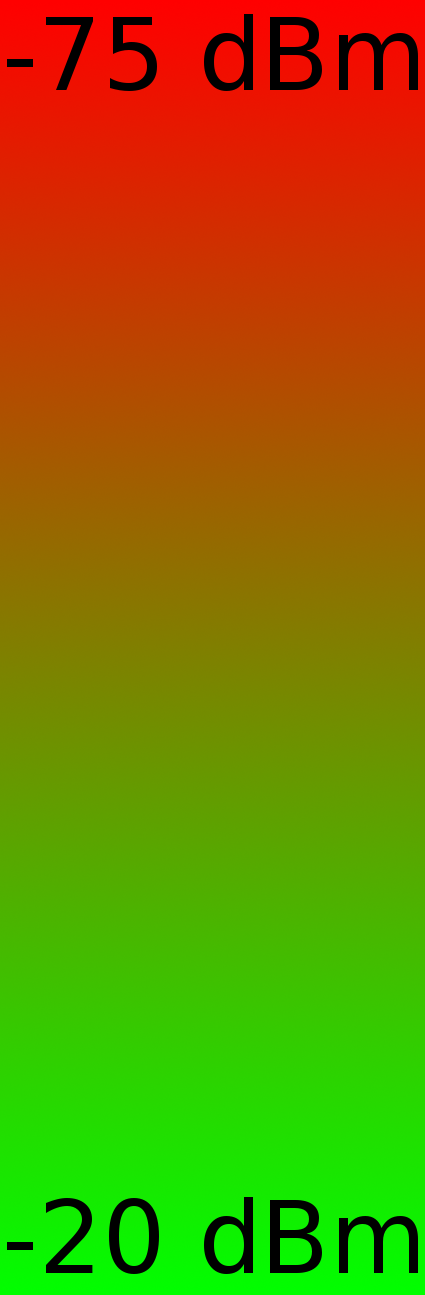
\includegraphics[scale=0.0275]{./figures/heatmap.png}}
              \vspace{-3mm}
    \caption{WiFi Heatmap, with and without the additional routers, for the ground and the second floor.}
\end{figure}








\begin{figure}[t!]     
    \subfloat[\scriptsize Glowing LEDs in night]{
        \label{fig:led}
        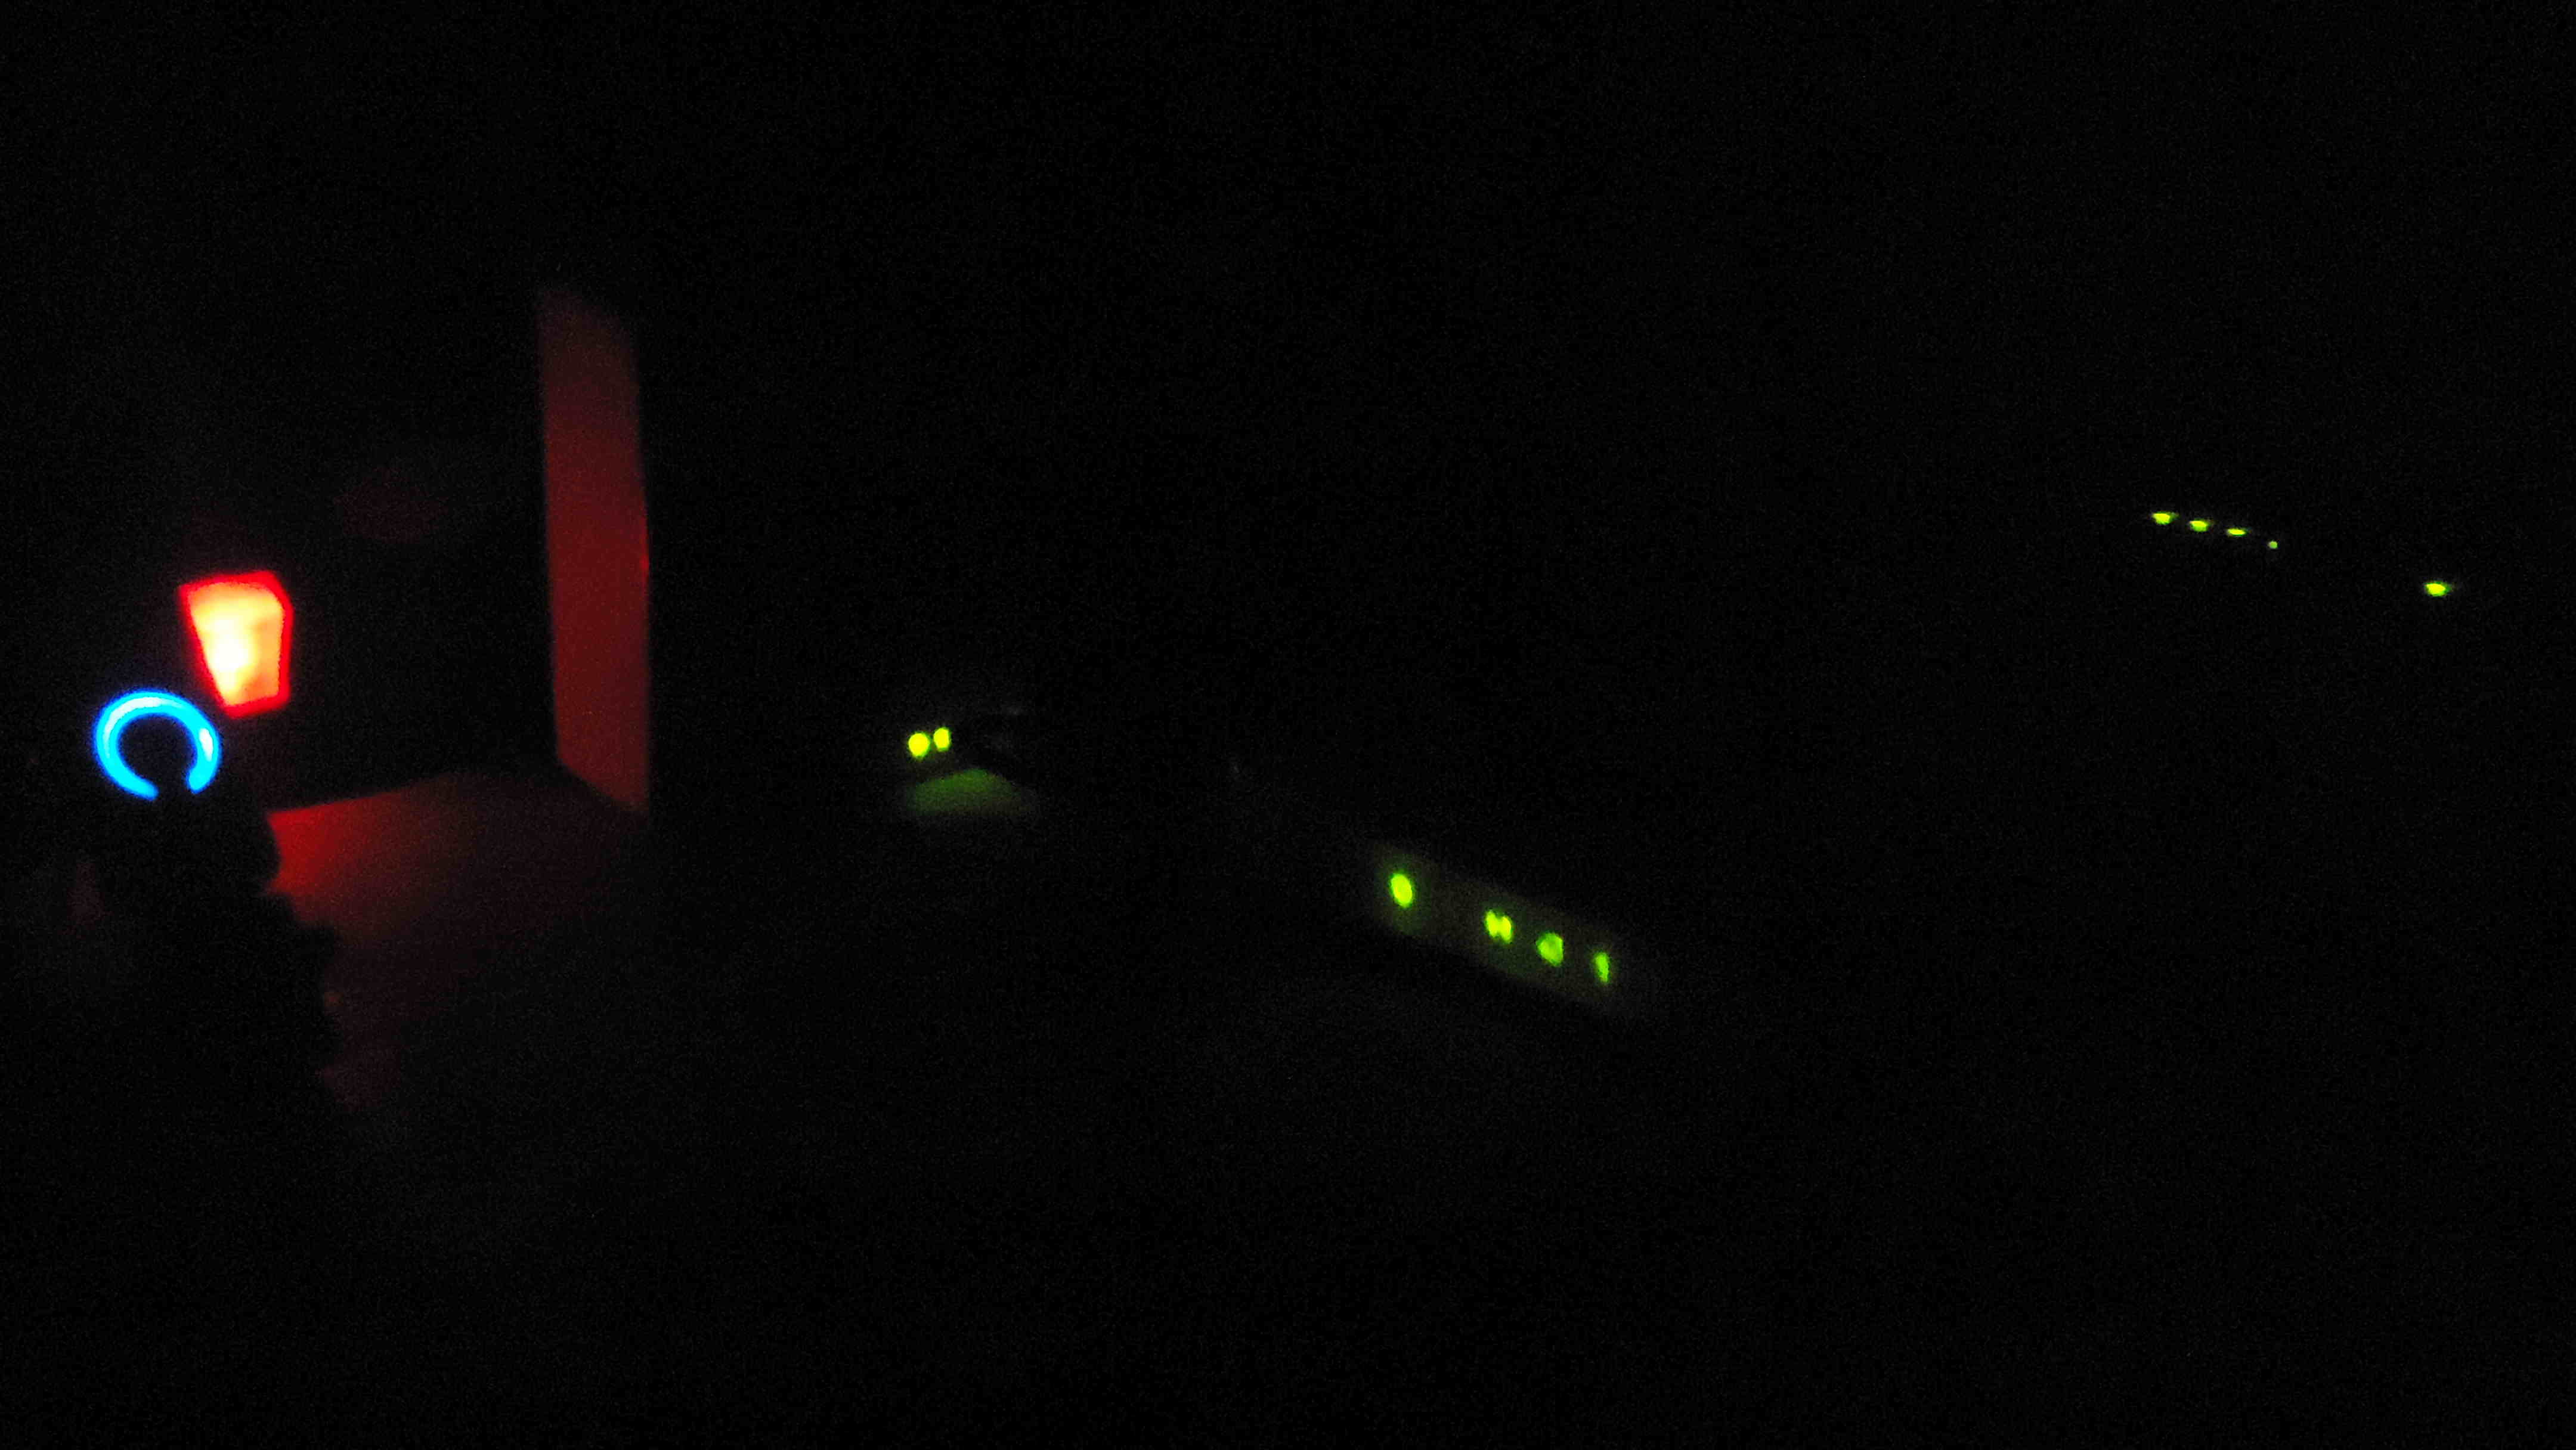
\includegraphics[scale=0.017]{./figures/led.jpg}}
        \hspace{0.02mm}
         \subfloat[\scriptsize Wire snag leading to data loss ]{
            \label{fig:snag}
            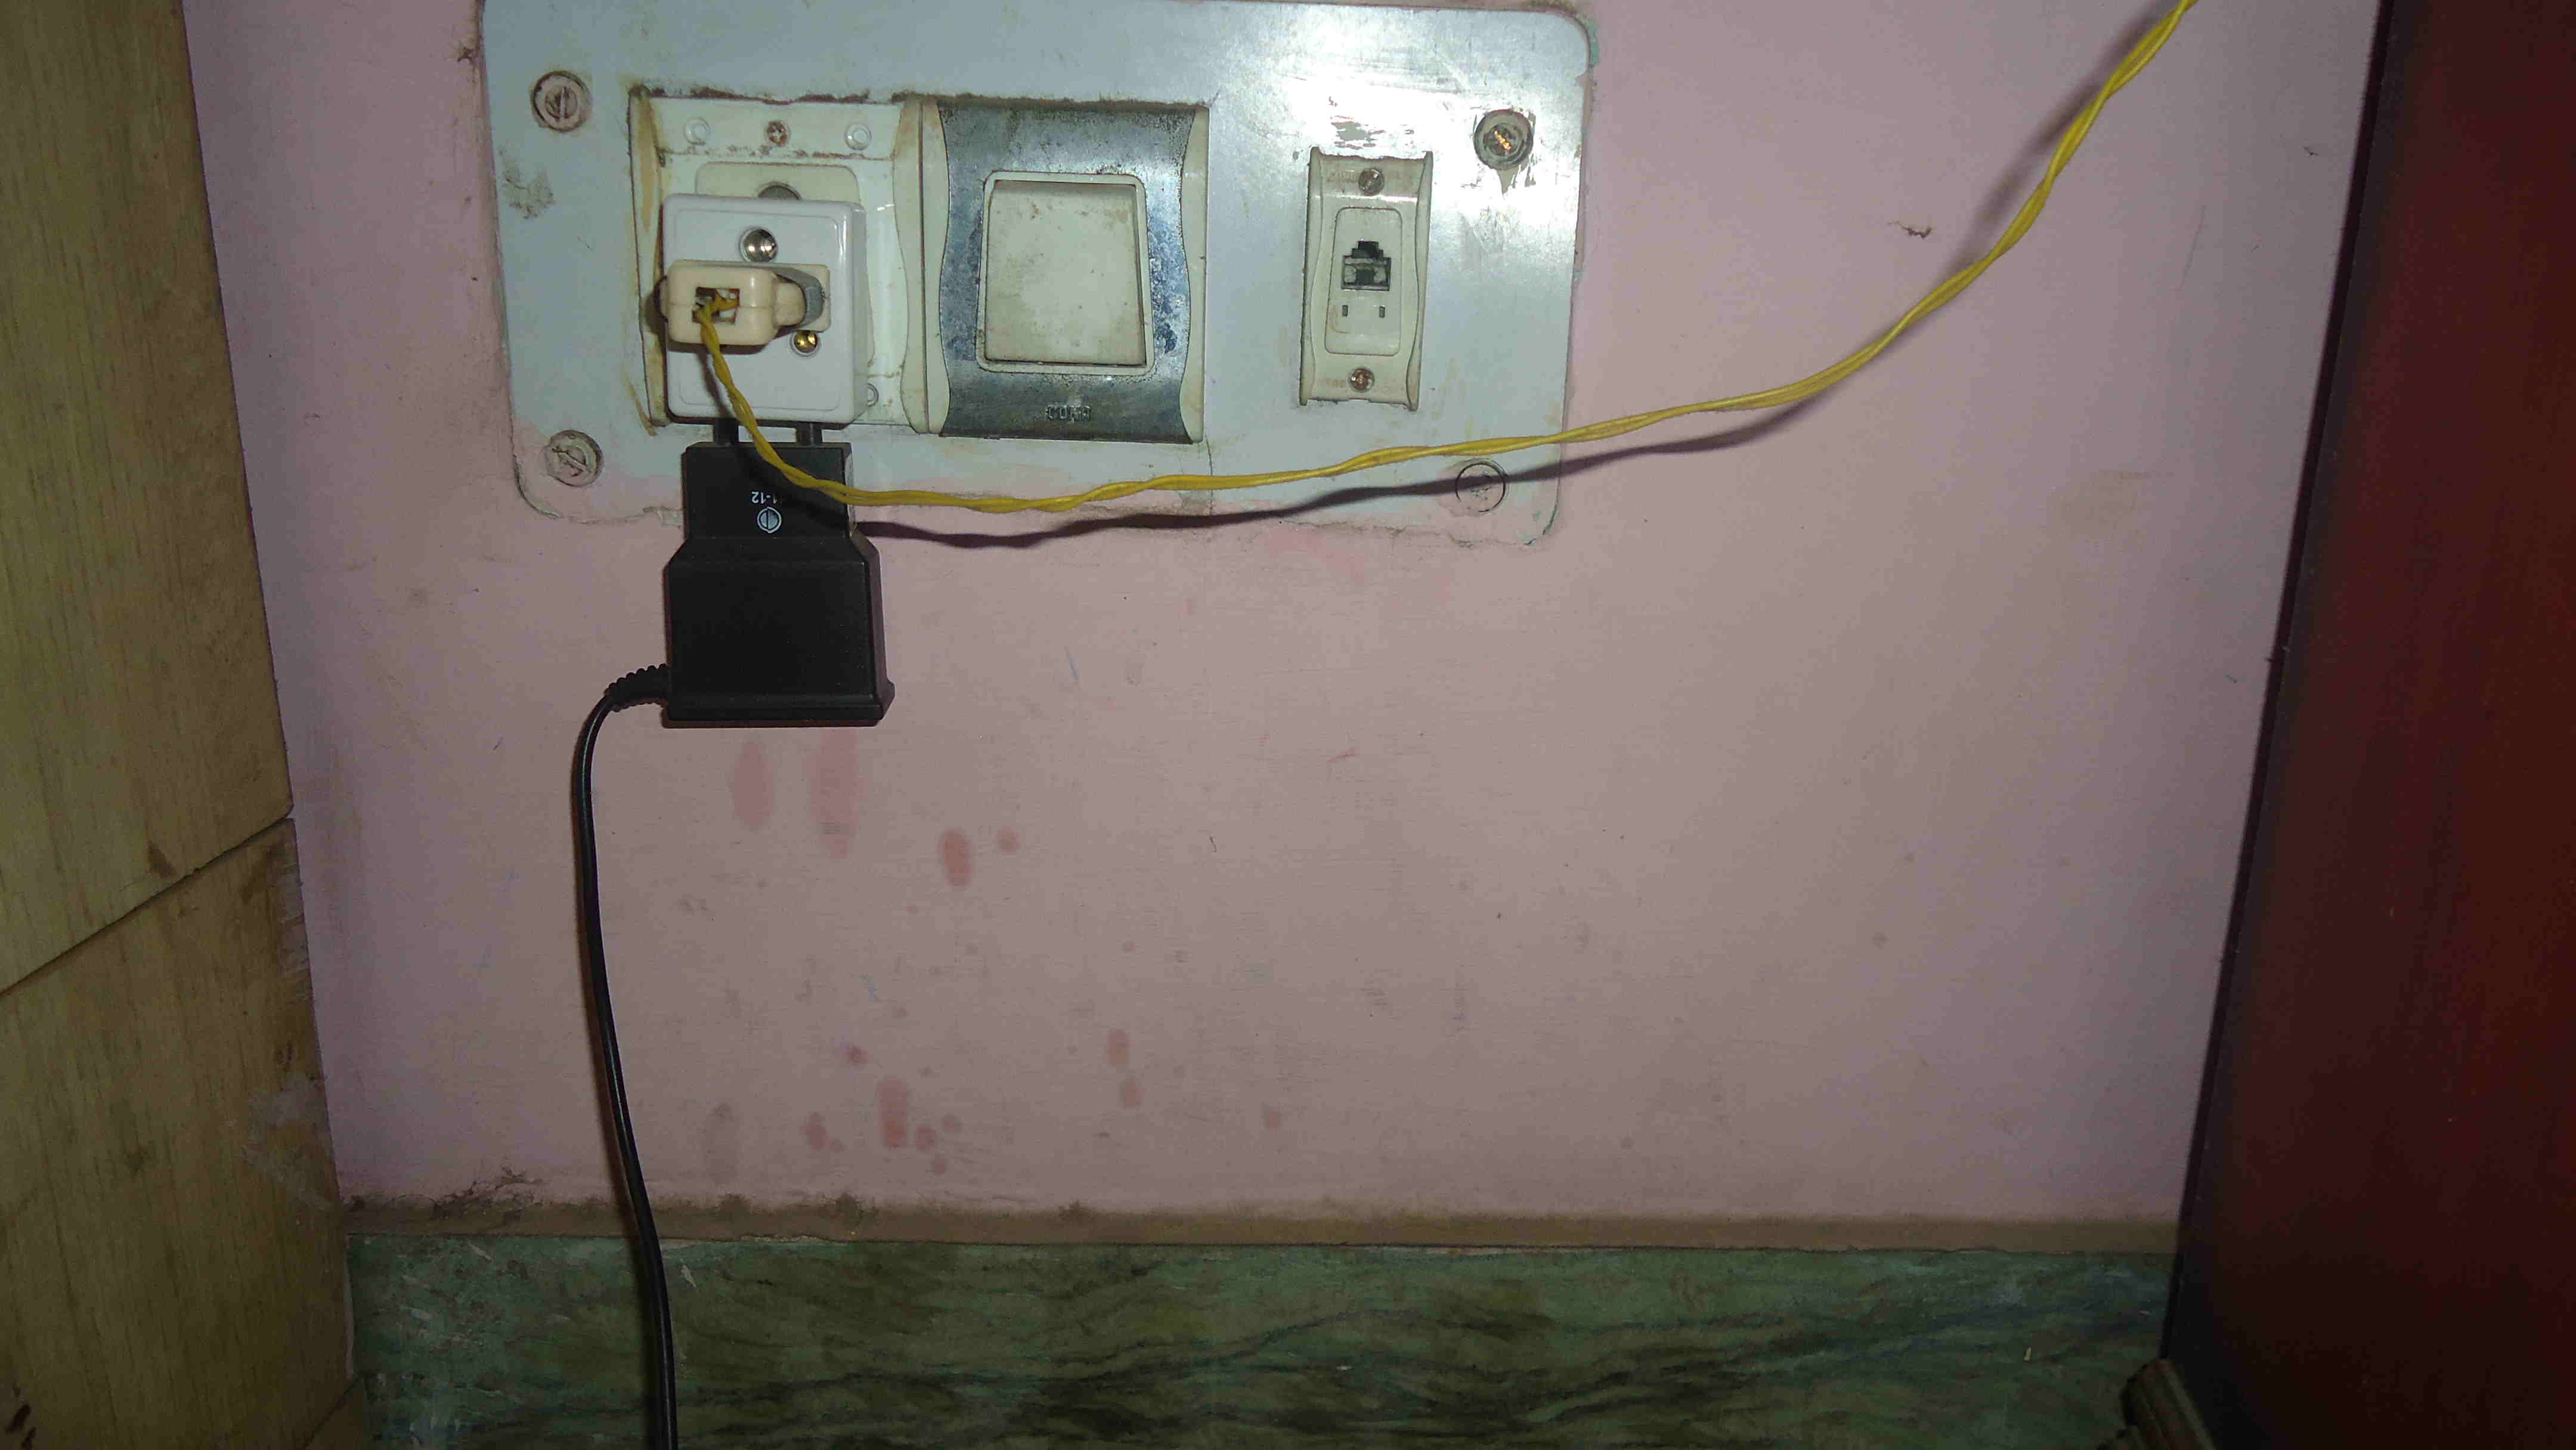
\includegraphics[scale=0.017]{./figures/snag.jpg}}
                    \hspace{0.02mm}
        \subfloat[\scriptsize Closely placed MCBs causing interference]{
                    \label{fig:ct_interference}
                    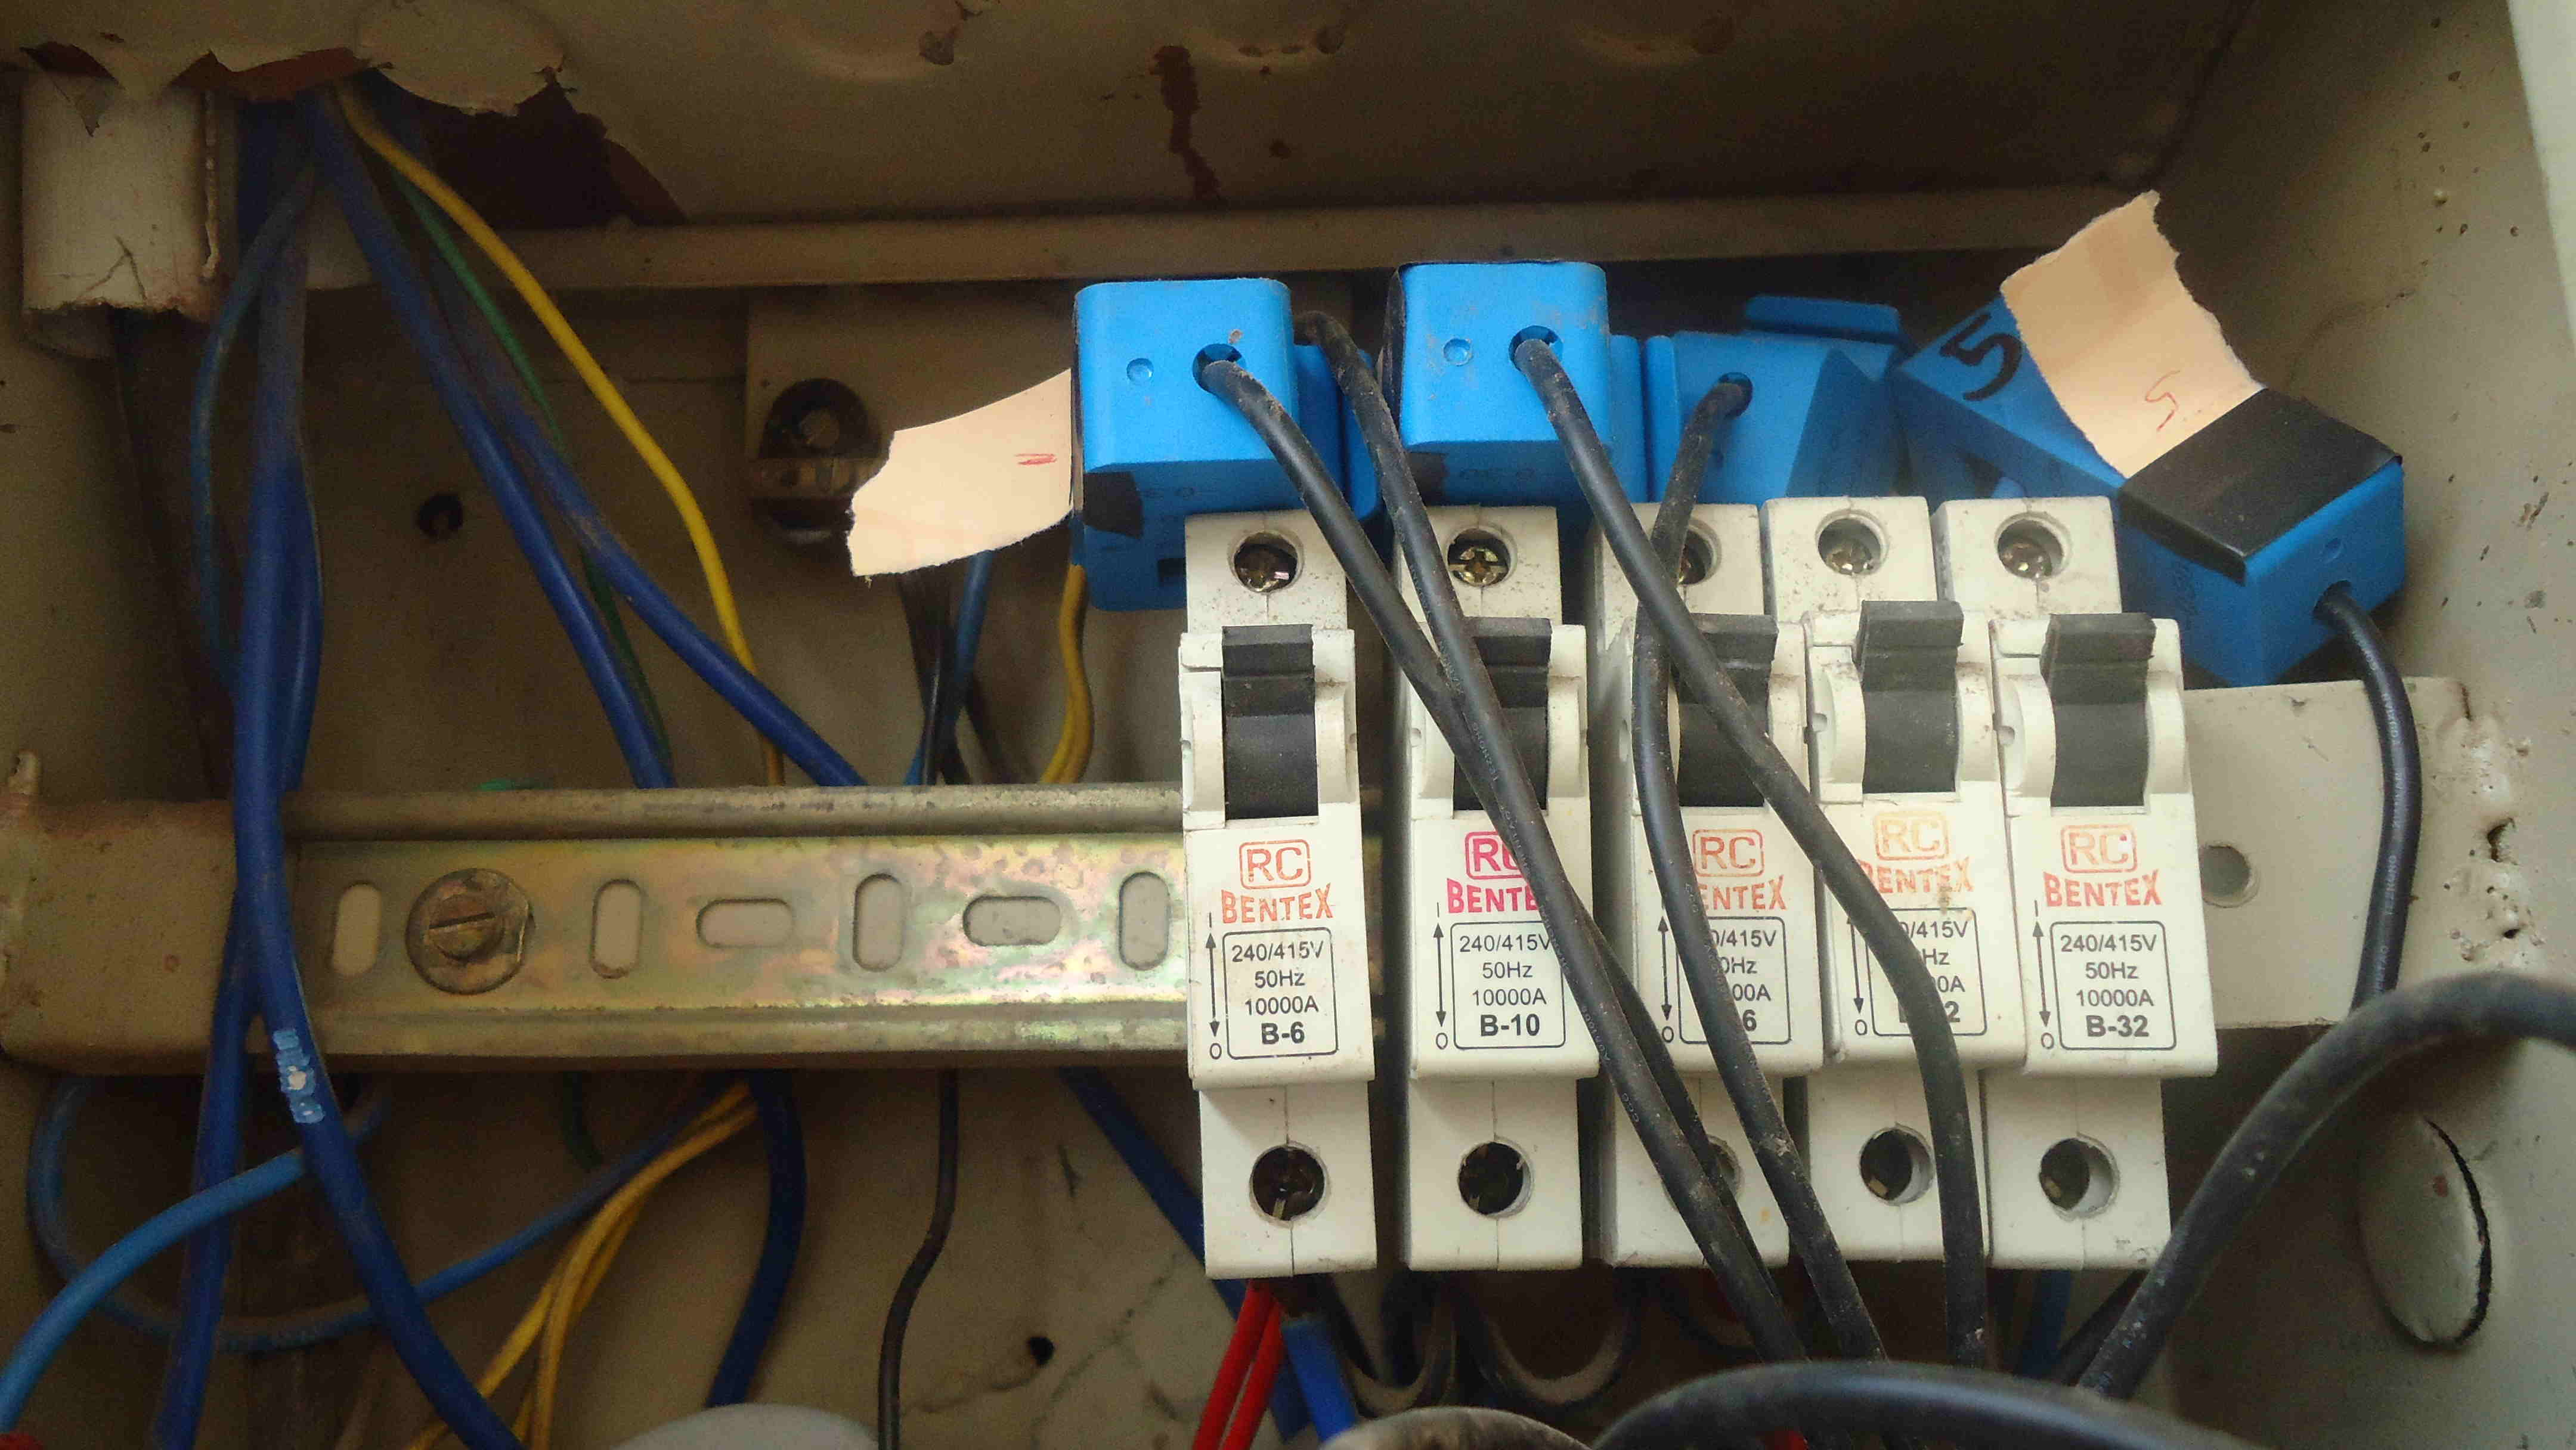
\includegraphics[scale=0.017]{./figures/ct_interference.jpg}}
                    \vspace{-3mm}
    \caption{Illustration of common problems}   
    \label{fig:home}
   \vspace{-3mm}
\end{figure}

\vspace{-1mm}
\section{Dataset and code release}
While we are working on complete annotation of the collected data, we are releasing fully labeled data for 1 day for open use. %This dataset is of the first of it's kind, across the world, where events corresponding to electricity, water and ambient sensors are timestamp recorded. 
We manually annotate the power consumed for each of the 63 appliances in their different states in the home. We similarly measure the amount of water consumed in 1 minute by each of the 18 water fixtures. We further provide a detailed metadata log for all the electrical appliances, including, approx. date of purchase, mapping to MCB, star-rating and rated power. All the appliance ON-OFF events can be easily captured using the plug level data collected from jPlug and Current Cost CT. 

\figref{fig:labeled} illustrates the advantage of detailed labeling together with use of multi-modal sensing. One of the occupants returned back home around 7:15 PM, an event captured synchronously by ground floor motion sensor, electricity meter and ground floor light sensor. The occupant (who was alone in the home) then heated up some food in the oven. While the oven jPlug failed to record it (due to the small usage time), this event is captured in the electricity meter data (spikes reaching up to 1800 watts). Thereafter, the occupant went to the first floor, turned on lights and switched on the laptop (illustrated through measurements from motion, light sensor on the first floor and laptop jPlug. After approx. an hour, the occupant switched on the air conditioner which is captured by the jPlug connected to the air conditioner as well as a spike in the meter measurements. Correspondingly, the temperature sensor in the room started observing reduced temperature values. 
 
%We intend to release more such fully labeled data in the future, but owing to privacy concerns, we limit the current fully labeled dataset to 1 day from this home. 
%While the accompanying switch had been to our disadvantage in measuring short duration appliance usage, it ensures that appliance ON-OFF events can be observed using jPlug data. 

\begin{figure} 
%	\vspace{-3mm}    
    \centering\includegraphics[scale=0.142]{./figures/label_annotated.png}
	\vspace{-2mm}    
    \caption{Utility of labeled and multi-modal dataset} 
    \vspace{-3mm}  
    \label{fig:labeled}
\end{figure}

We also publicly release our codebase which includes \selstups implementation, scripts for collecting data from different sensors, database schemas, soft-sensors, startup scripts and the fixes we developed for common problems on RPi. Our codebase and dataset is available on Github\footnote{\url{http://github.com/nipunreddevil/Home_Deployment}}.

\vspace{-1mm}
\section{Conclusions and Future Work}
\looseness -1 In this paper, we present our experiences with an extensive residential deployment monitoring electrical, water and ambient parameters in Delhi, India. To the best of our knowledge, this is the first extensive residential deployment in a developing country. We present key aspects of our deployment and discuss the corresponding impact on the design of building monitoring and control systems that aim to scale across diverse contexts offered in the developing and the developed countries. Some of the unique aspects, impacting the systems development in building energy domain, include - unreliable electrical grid, unreliable network connectivity, decentralized electrical loads and energy-water nexus within a home. We further discussed the similarities in our learning with prior work (done in the USA), demystifying the home environment for energy and water related deployments in the Indian context. %importance of poor wireless connectivity in homes and the importance of aesthetics.

Frequent power outages and unreliable internet motivated us to develop the proposed sensing architecture: \selstup, which accounts for these pitfalls by introducing local storage and periodic upload. Such an architecture can be of particular importance for scaling the building monitoring and control systems for applicability across diverse contexts. %suitable for the developing countries. 
We are in the process of installing our sensors across multiple other homes in Delhi. Detailed, annotated data from the deployment will be released for public use after necessary post processing and filtering. We further plan to carry out longer duration deployments capturing seasonal variations in the energy usage patterns. %and after that we wish to release our data set in the public. 
%We are also developing a billing application for providing detailed electricity usage information to home owners. 
%We plan to perform NILM and provide the home occupants with detailed electricity consumption breakdown.

\balance
%\vspace{-2mm}
\bibliographystyle{abbrv}
\bibliography{references} 

\end{document}
